% !TEX TS-program = xelatexmk
\documentclass[twoside,12pt]{Latex/Classes/PhDthesisPSnPDF}


%: Macro file for Latex
% Macros help you summarise frequently repeated Latex commands.
% Here, they are placed in an external file /Latex/Macros/MacroFile1.tex
% An macro that you may use frequently is the figuremacro (see introduction.tex)
% This file contains macros that can be called up from connected TeX files
% It helps to summarise repeated code, e.g. figure insertion (see below).

% insert a centered figure with caption and description
% parameters 1:filename, 2:title, 3:description and label
\newcommand{\figuremacro}[3]{
	\begin{figure}[htbp]
		\centering
		\includegraphics[width=1\textwidth]{#1}
		\caption[#2]{\textbf{#2} - #3}
		\label{#1}
	\end{figure}
}

% insert a centered figure with caption and description AND WIDTH
% parameters 1:filename, 2:title, 3:description and label, 4: textwidth
% textwidth 1 means as text, 0.5 means half the width of the text
\newcommand{\figuremacroW}[4]{
	\begin{figure}[htbp]
		\centering
		\includegraphics[width=#4\textwidth]{#1}
		\caption[#2]{\textbf{#2} - #3}
		\label{#1}
	\end{figure}
}

% inserts a figure with wrapped around text; only suitable for NARROW figs
% o is for outside on a double paged document; others: l, r, i(inside)
% text and figure will each be half of the document width
% note: long captions often crash with adjacent content; take care
% in general: above 2 macro produce more reliable layout
\newcommand{\figuremacroN}[3]{
	\begin{wrapfigure}{o}{0.5\textwidth}
		\centering
		\includegraphics[width=0.48\textwidth]{#1}
		\caption[#2]{{\small\textbf{#2} - #3}}
		\label{#1}
	\end{wrapfigure}
}

% predefined commands by Harish
\newcommand{\PdfPsText}[2]{
  \ifpdf
     #1
  \else
     #2
  \fi
}

\newcommand{\IncludeGraphicsH}[3]{
  \PdfPsText{\includegraphics[height=#2]{#1}}{\includegraphics[bb = #3, height=#2]{#1}}
}

\newcommand{\IncludeGraphicsW}[3]{
  \PdfPsText{\includegraphics[width=#2]{#1}}{\includegraphics[bb = #3, width=#2]{#1}}
}

\newcommand{\InsertFig}[3]{
  \begin{figure}[!htbp]
    \begin{center}
      \leavevmode
      #1
      \caption{#2}
      \label{#3}
    \end{center}
  \end{figure}
}


%PACKAGES
%math
\usepackage{amsmath}
\usepackage{bbold}

\usepackage{xfrac}
\usepackage{mathrsfs}

\usepackage{slashed}
\usepackage{simplewick}

\usepackage{braket}

\usepackage{upgreek}

%for points in graphics filenames
\usepackage{grffile}

% for sideways figures
\usepackage{rotating}

%prevent figures moving around too much
\usepackage{placeins}

%single spacing
\usepackage{setspace}

\newcommand \sgroup[2]{\mathrm{#1}(#2)}
\newcommand \uone {\sgroup{U}{1}}
\newcommand \su[1]{\sgroup{SU}{#1}}

\newcommand \LL{\mathrm{L}}
\newcommand \bigL {\mathscr{L}}
\newcommand \lag[1] {\bigL_{\mathrm{#1}}}

\newcommand\emm{\mathrm{M}}
\newcommand\pmp{\psi_{\emm+}}
\newcommand\pmm{\psi_{\emm-}}
\newcommand\pb{\overline{\psi}}
\newcommand\pbmp{\pb_{\emm+}}
\newcommand\pbmm{\pb_{\emm-}}
\newcommand\Tr{\mathrm{T}}
\newcommand\Tra{\mathrm{tr}}
\newcommand\one{\mathbb{1}}

\newcommand\dslash{\slashed{\partial}}
\newcommand\Dslash{\slashed{D}}	

\newcommand \Nx[1]{N_\mathrm{#1}}
\newcommand \Nf {\Nx{f}}
\newcommand \scrM {\mathscr{M}}

\usepackage[font=footnotesize]{subcaption}


%SHORTHANDS
%MATH
%\newcommand \dim{\mathrm{dim}}
\newcommand \NfR[1]{\Nf^{\mathrm{#1}}[\rep{R}]}
\newcommand\Gb{\overline{\Gamma}}
\newcommand\nubar{\overline{\nu}}
\newcommand\LR{\mathrm{L(R)}}
%TEXT
\newcommand \lmwt {$\su{2}$Adj\,Nf1\xspace}
\newcommand \mwt {Minimal Walking Technicolor\xspace}

%Words that are easy to misspell so should be in commands
\usepackage{xspace}
\hyphenation{BSMBench}
\newcommand \bsmbench {BSMBench\xspace}
\newcommand \blueice {BlueIce2\xspace}
\newcommand \spinhalf {spin-$\frac{1}{2}$\xspace}
\newcommand \xsb {$\upchi$SB\xspace}

%TABLES
\usepackage{footnote}
\usepackage{pbox}
\usepackage{tabularx}
\newcolumntype{Y}{>{\centering}X}
\newcolumntype{y}{>{\centering\arraybackslash}X}


%COMMANDS TO FIDDLE WITH MARGIN NOTES – UNCOMMENT SECOND TO DISABLE THEM FOR SUBMISSION
\usepackage{marginnote}
%\let \marginnoteold \marginnote
%\renewcommand\marginnote[1]{\marginnoteold[#1]{}}

%FONT-RELATED ENVIRONMENTS
\newcommand \Sx[1]{S_{\textnormal{#1}}}
\newcommand \rep[1]{\mathrm{#1}}

\newcommand\nojustno[1]{}




%SET UP HEADING FONTS
%\usepackage{titlesec}
%\titleformat{\chapter}[display]
%  {\fontspec{Cosmos}\huge\bfseries}
%  {\chaptertitlename\ \thechapter}{8pt}{\Huge}
%\titleformat*{\section}{\Large\bfseries\fontspec{Cosmos}}
%\titleformat*{\subsection}{\large\bfseries\fontspec{Cosmos}}
%\titleformat*{\subsubsection}{\itshape\bfseries\fontspec{Cosmos}}


%DISABLE MARGIN NOTES
%\renewcommand \marginnote[1] {}

%%% Local Variables: 
%%% mode: latex
%%% TeX-master: "~/Documents/LaTeX/CUEDThesisPSnPDF/thesis"
%%% End: 


\usepackage{kpfonts}
\usepackage{epigraph}
\usepackage{float}
%: ----------------------------------------------------------------------
%:                  TITLE PAGE: name, degree,..
% ----------------------------------------------------------------------
% below is to generate the title page with crest and author name

%if output to PDF then put the following in PDF header
\ifpdf  
    \pdfinfo { /Title  (Matter in 2+1 dimensions at finite density with Chern-Simons interactions)
               /Creator (TeX)
               /Producer (XeLaTeX)
               /Author (Stanislav Stratiev StanislavStratiev@gmail.com)
               /CreationDate (D:202003158000)  %format D:YYYYMMDDhhmmss
               /ModDate (D:201310081042)
               /Subject (Subject)
               /Keywords () }
    \pdfcatalog { /PageMode (/UseOutlines)
                  /OpenAction (fitbh)  }
\fi


\title{Matter in 2+1 Dimensions at Finite Density with Chern-Simons Interactions}



%\ifpdf
  \author{\href{mailto:StanislavStratiev@gmail.com}{Stanislav Stratiev}}
  \collegeordept{\href{http://www.swansea.ac.uk/physics}{Department of Physics}}
  \university{\href{http://www.swansea.ac.uk}{Swansea University}}

  % The crest is a graphics file of the logo of your research institution.
  % Place it in ./Front_Folder/figures and specify the width
  \crest{
\includegraphics[width=4cm]{logo.pdf}}
  
% If you are not creating a PDF then use the following. The default is PDF.
%\else
%  \author{YourName}
%%  \cityofbirth{born in XYZ}
%  \collegeordept{CollegeOrDept}
%  \university{University}
%  \crest{
\includegraphics[width=4cm]{logo}}
%\fi

\renewcommand{\submittedtext}{Submitted to Swansea University in fulfilment \\ of the requirements for the degree of}
\degree{Doctor of Philosophy}
\degreedate{2020}


% ----------------------------------------------------------------------
       
% turn of those nasty overfull and underfull hboxes
\hbadness=10000
\hfuzz=50pt


%: --------------------------------------------------------------
%:                  FRONT MATTER: dedications, abstract,..
% --------------------------------------------------------------
%\usepackage[xelatex]{graphicx}
\usepackage{eso-pic}
\usepackage{tikz}
\usepackage{bm}
\def\mg{{\mathfrak g}}
\newcommand{\MAT}[1]{\begin{pmatrix} #1\end{pmatrix}}
\newcommand{\EQ}[1]{\begin{equation}\begin{split} #1
\end{split}\end{equation}}
\def\ben
{\begin{equation}}
\def\een{\end{equation}}
\def\half{{\textstyle{1\over2}}}
\def\p{{\bf p}}
\def\U{\text{U}}
\let\a=\alpha \let\b=\beta \let\g=\gamma \let\d=\delta \let\e=\varepsilon
\let\z=\zeta \let\h=\eta \let\q=\theta \let\k=\kappa
\let\l=\lambda \let\m=\mu \let\n=\nu \let\x=\xi \let\r=\rho
\let\s=\sigma \let\t=\tau \let\u=\upsilon \let\c=\chi
\let\y=\psi
\let\w=\mu \let\G=\Gamma \let\D=\Delta \let\Q=\Theta \let\L=\Lambda
\let\X=\Xi \let\P=\Phi  \let\Y=\Psi
\let\C=\Chi \let\W=\mu
\let\la=\label \let\ci=\cite \let\re=\ref
\let\se=\section \let\sse=\subsection \let\ssse=\subsubsection
\def\nn{\nonumber}
\let\fr=\frac
\def\W={\cal W}
\def\L ={\cal L}
\let\na=\nablal
\let\pa=\partial
\def\be{\begin{equation}}
\def\ee{\end{equation}}
\def\ba{\begin{array}}
\def\ea{\end{array}}
\def\del{\partial}
\def\vp{\varphi}
\def\td{\tilde}
\def\wtd{\widetilde}
\def\ie{\rm i.e.\ }
\def\dalemb#1#2{{\vbox{\hrule height .#2pt
        \hbox{\vrule width.#2pt height#1pt \kern#1pt
                \vrule width.#2pt}
        \hrule height.#2pt}}}
\def\square{\mathord{\dalemb{6.8}{7}\hbox{\hskip1pt}}}
\newcommand{\bea}{\begin{eqnarray}}
\newcommand{\eea}{\end{eqnarray}}
\newcommand{\tr}{{\rm tr} }
\newcommand{\Tr}{{\rm Tr} }
\newcommand{\mf}{\mathfrak}
\newcommand{\sh}[1]{#1\hskip-7pt /}
\newcommand{\rqm}{{%
\declareslhed{}{\text{/}}{0.04}{0}{k}\slashed{k}}}
\newcommand\BackgroundPic{
\put(0,0){
\parbox[b][\paperheight]{\paperwidth}{%
\vfill
\centering
\begin{tikzpicture}[remember picture, overlay]
 \node[inner sep=0pt] at (current page.center) {%
  
\includegraphics[width=\paperwidth,height=\paperheight]{background.pdf}%
};
\end{tikzpicture}
\vfill
}}}

\reversemarginpar

      
\begin{document}
\AddToShipoutPicture*{\BackgroundPic}

%\language{english}

% sets line spacing
\renewcommand\baselinestretch{1.2}
\baselineskip=18pt plus1pt



%: ----------------------- generate cover page ------------------------

\maketitle  % command to print the title page with above variables

%\newpage

%: ----------------------- abstract ------------------------
\renewcommand\marginnote[1]{}

% Thesis Abstract -----------------------------------------------------


%\begin{abstractslong}    %uncommenting this line, gives a different abstract heading
\begin{abstracts}        %this creates the heading for the abstract page

\begin{singlespace}
    We study several matter Chern-Simons models at finite chemical potential. In the SU(N) theory we discover a color-flavour locking Bose condensed ground state with vacuum expectation values for both the scalars and the gauge fields. We identify this ground state with the non-commutative Chern-Simons description of the quantum hall effect. We compute the quadratic spectrum and discover roton excitations. We find a self-consistent circularly symmetric ansatz for topological non-abelian vortices. We examine vortices in Abelian Chern-Simons theory coupled to a relativistic scalar field with a chemical potential for particle number or U(1) charge. The Gauss constraint requires chemical potential for the local symmetry to be accompanied by a constant background charge density/magnetic field. Focusing attention on power law scalar potentials $∼ |\Phi|^{2s}, \, s\in \mathbb{Z}$ which do not support vortex configurations in vacuum but do so at finite chemical potential, we numerically study classical vortex solutions for large winding number $|n|\gg  1$.
\end{singlespace}

\end{abstracts}
%\end{abstractlongs}


% ---------------------------------------------------------------------- 



%: ----------------------- cover page back side ------------------------
% Your research institution may require reviewer names, etc.
% This cover back side is required by Dresden Med Fac; uncomment if needed.


%: Declaration of originality

% Thesis statement of originality -------------------------------------

% Depending on the regulations of your faculty you may need a declaration like the one below. This specific one is from the medical faculty of the university of Dresden.

%\begin{declaration}        %this creates the heading for the declaration page

\newcommand{\signeddate}{
\vskip 30pt Signed: \dotfill (candidate)

\vskip 20pt Date: \dotfill\hphantom{ (candidate)}}

\vskip 10pt
\subsection*{Declaration}
This work has not previously been accepted in substance for any degree and is not being concurrently submitted for any degree.

\signeddate

\vskip 40pt
\subsection*{Statement 1}
This thesis is the result of my own investigations, except where otherwise stated. Where correction services have been used, the extent and nature of the correction is clearly marked in a footnote(s).
Other sources are acknowledged by footnotes giving explicit references. A bibliography is appended.

\signeddate

\vskip 40pt
\subsection*{Statement 2}
I hereby give consent for my thesis, if accepted, to be available for photocopying and for inter-library loan, and for the title and summary to be made available to outside organisations.

\signeddate


%\end{declaration}


% ----------------------------------------------------------------------



% The original template provides and abstractseparate environment, if your institution requires them to be separate. I think it's easier to print the abstract from the complete thesis by restricting printing to the relevant page.
% \begin{abstractseparate}
%   
% Thesis Abstract -----------------------------------------------------


%\begin{abstractslong}    %uncommenting this line, gives a different abstract heading
\begin{abstracts}        %this creates the heading for the abstract page

\begin{singlespace}
    We study several matter Chern-Simons models at finite chemical potential. In the SU(N) theory we discover a color-flavour locking Bose condensed ground state with vacuum expectation values for both the scalars and the gauge fields. We identify this ground state with the non-commutative Chern-Simons description of the quantum hall effect. We compute the quadratic spectrum and discover roton excitations. We find a self-consistent circularly symmetric ansatz for topological non-abelian vortices. We examine vortices in Abelian Chern-Simons theory coupled to a relativistic scalar field with a chemical potential for particle number or U(1) charge. The Gauss constraint requires chemical potential for the local symmetry to be accompanied by a constant background charge density/magnetic field. Focusing attention on power law scalar potentials $∼ |\Phi|^{2s}, \, s\in \mathbb{Z}$ which do not support vortex configurations in vacuum but do so at finite chemical potential, we numerically study classical vortex solutions for large winding number $|n|\gg  1$.
\end{singlespace}

\end{abstracts}
%\end{abstractlongs}


% ---------------------------------------------------------------------- 

% \end{abstractseparate}

%\frontmatter

%: ----------------------- contents ------------------------

\setcounter{secnumdepth}{3} % organisational level that receives a numbers
\setcounter{tocdepth}{3}    % print table of contents for level 3
\tableofcontents            % print the table of contents
% levels are: 0 - chapter, 1 - section, 2 - subsection, 3 - subsection


%: ----------------------- tie in front matter ------------------------

% Thesis Acknowledgements ------------------------------------------------


%\begin{acknowledgementslong} %uncommenting this line, gives a different acknowledgements heading
\begin{acknowledgements}      %this creates the heading for the acknowlegments

    I'd like to thank Prem Kumar for his patient supervision over the past few years.
\end{acknowledgements}
%\end{acknowledgmentslong}

% ------------------------------------------------------------------------







%: ----------------------- list of figures/tables ------------------------

\listoffigures	% print list of figures

\listoftables  % print list of tables


%: --------------------------------------------------------------
%:                  MAIN DOCUMENT SECTION
% --------------------------------------------------------------

% the main text starts here with the introduction, 1st chapter,...
\mainmatter

%\renewcommand{\chaptername}{} % uncomment to print only "1" not "Chapter 1"


%: ----------------------- subdocuments ------------------------

% Parts of the thesis are included below. Rename the files as required.
% But take care that the paths match. You can also change the order of appearance by moving the include commands.


\let\oldleftmark=\leftmark
\let\oldrightmark=\rightmark
    \renewcommand{\leftmark}{INTRODUCTION}
    \renewcommand{\rightmark}{INTRODUCTION}
\addcontentsline{toc}{chapter}{Introduction}

% this file is called up by thesis.tex
% content in this file will be fed into the main document
    \graphicspath{{Introduction_Folder/figures/PNG/}{Introduction_Folder/figures/PDF/}{Introduction_Folder/figures/}}

%: ———————-- introduction file header ———————--
\chapter*{Introduction}

On the second day of my graduate studies, The Nobel prize in Physics was awarded to D. Thouless, M. Kosterlitz and D. Haldane for the discovery of topological phase transitions\footnote{https://www.nobelprize.org/prizes/physics/2016/summary/}. At the time I thought topology was a subject about open neighbourhoods, hausdorff spaces and counting holes on mugs and doughnuts. I could not fathom how these ideas could have anything to do with the description of the real world. I had to understand how these concepts were connected. This thesis follows my path of exploring the mystery of topological physics from the perspective of high energy physics and quantum field theory (QFT).

Today, topology has become ubiquitous in the study of physics. It provides us with new models to gain insight into nature. In addition, it provides the stability for new kinds of excitations in models whose initial purpose had more to do with the study of particles \textcolor{red}{(For example, topological degrees of freedom were discovered in the Glashow-Salam model by 't Hooft \& Polyakov in 1974 \cite{Polyakov:1974ek, tHooft:1974kcl})}. Even very deep questions such as the understanding of confinement and the attempts to study strongly correlated gauge theories seem to be intimately related to the study of continuous deformations. There are hints that confinement might be related to instanton condensation \cite{Polyakov1977}. And most relevant to this work, it seems that the promising path of relating strongly and weakly coupled theories through dualities, relate the conserved current of a theory to the topological current of its dual. It was our hope that we can shed some more light on the details of these dualities at finite matter density and for this reason, this thesis has been centered around the study of the grand canonical ensemble of Chern-Simons matter theories, specifically scalar field theories.

The first novelty that we stumbled upon was a ground state that had been overlooked since it only manifests itself in the finite chemical potential regime. It is a ground state with non-zero expectation value for the gauge fields, seemingly breaking rotational symmetry. In reality, color-flavor locking remedies this and the rotational symmetry is preserved. In order to confirm this, we also computed the quadratic spectrum of the theory, which showed no signs of rotational asymmetry. We discovered further, owing to Goldstone's theorem and the broken $U(1)_B$ global symmetry, that the long wave-length dynamics of the SU(2) theory behaved as a superfluid and predicts the existence of a roton excitation. What was even more surprising is that this non-trivial ground state exists in the zero coupling free scalar theory coupled to Chern-Simons. This is peculiar since we generally expect there to be a potential that drives the symmetry breaking.

Correlation functions for the scalar Chern-Simons theory at $\mu=0$ have been computed exactly in the large $N$ limit \cite{Aharony:2012nh}. Since the $\mu =0$ results cannot be extrapolated to finite $\mu$, we would need to take the ground state discussed in the previous paragraph into account. A natural question that arises is what do the correlation functions look like in the presence of this new condensate at large $N$? This was the ultimate aim that we \textcolor{red}{had} in commencing this work, \textit{i.e.} solving this theory in the large $N$ limit. In order to pursue this direction, we set ourselves the more conservative goal of computing the quadratic spectrum in the general $N$ SU(N) theory. The ground state in the SU(N) theory has the same algebraic structure as the non-commutative Chern-Simons theory used as a model for the FQHE. The approach to diagonalizing the large $N$ spectrum of fluctuations that we outlined involves translating the problem to a non-commutative Chern-Simons theory and using the solutions of that model to arrive at an exact result.

    Aside from studying the ground state and the fundamental excitations of finite density Chern-Simons models, we have also explored the existence and properties of solitons (vortices) in these models. Our main results in this line are the discovery and study of an approximate numerical BPS state in the abelian theory. Additionally, we find a self consistent vortex ansatz for the SU(2) and U(2) theories. We have left the numerical study of the resulting equations for future work.

    This thesis is structured in the following way:

    In Chapter 1, we cover the necessary background required to understand the rest of the thesis and how it fits in the wider field of research. We present a condensed introduction to the topics of Chern-Simons field theory, the Quantum Hall effect, vortices, particle-vortex duality, Fermi-Bose duality, the statistical grand canonical ensemble in quantum field theory and non-commutative field theory.

    Chapter 2 presents the analytical and numerical study of abelian vortex solutions interpolating between a symmetric and asymmetric phase, where the symmetry breaking is chemical potential driven.

    Chapter 3 showcases the derivation of the peculiar ground state mentioned earlier, the spectrum of fluctuations is analyzed in the SU(2) theory. The chapter concludes with the SU(N) ground state and the observation that it resembles non-commutative Chern-Simons theory.

    In Chapter 4 we switch gears back to vortices, except this time we consider the possibility of topological solutions in the non-abelian theory. We show that there is a self-consistent circularly symmetric ansatz for a global vortex in the SU(2) theory and a local vortex in the U(2) theory.

%This will be the introduction chapter. I will talk about:
%
%
%
%\begin{itemize}
%    \item The reunion of QFT and CMT that has been sparked in recent years by studies such as dualities
%    \item Importance of topological field theory in practice. Quantum Computing and \textit{etc}. 
%    \item Most importantly, highlight the importance of studying dualities as a tool to understand strongly coupled field theories. Deforming well known dualities and attempting to match the two sides takes us closer to having dual descriptions of theories that are of physical interest.
%    \item 
%\end{itemize}
	% background information
    \pagebreak
    \let\leftmark=\oldleftmark
    \let\rightmark=\oldrightmark

% this file is called up by thesis.tex
% content in this file will be fed into the main document
    \graphicspath{{Background_Folder/figures/PNG/}{Background_Folder/figures/PDF/}{Background_Folder/figures/}}

%: ———————-- introduction file header ———————--
\chapter{Background}
This chapter provides the necessary background \colorbox{red}{information} and technical \colorbox{red}{details} required to understand the main results of this thesis and their implications to related fields of physics. These include both the theoretical framework we will use and the real world phenomena to which it relates to. As should already be clear by now, in this text, we will concern ourselves with the study of planar systems at finite density. We will approach the study of these two dimensional systems through the framework of Quantum Field Theory (QFT). 

    There are two important aspects of QFT that will play a major role for us. One of them is the relation between the grand canonical statistical partition function and QFT. The other aspect is the distinct way in which the gauge principle manifests itself in 2+1 dimensional theories. The latter is addressed in \textcolor{red}{section} \ref{CS_sec}, where we review the basics of \textit{Chern-Simons theory}. The former is discussed in \textcolor{red}{section} \ref{GCE_sec}, where we will spend time reminding ourselves \colorbox{red}{of} some basic statistical mechanics. 

   % After we have covered these, we will turn to the physics this formalism aims to address in \ref{phys_app_sec}. We will review the \textit{Landau-Ginzburg  paradigm} \ref{Landau-Ginzburg_sec} of symmetry breaking and phase transitions, its inability to account for all phases observable in nature and where topological phases of matter fit in this picture.

    After we have covered these, \colorbox{red}{ }we will spend some time looking at the problems of the \textit{fractional and integer quantum hall effects} (FQHE/IQHE) in \textcolor{red}{section} \ref{FQHE_sec} and emphasize \colorbox{red}{their} relation to Chern-Simons matter theories. This will help us understand the applications and motivate the study of the models we are concerned with in this text.

    Then, we shall continue by reviewing the properties of \textit{vortices} in section \ref{vortices_sec}. Specifically, we look at vortices in the abelian Higgs model, Pure abelian Chern-Simons theory with scalar matter and the mixed case where both $S_{\text{Maxwell}}$ and $S_{\text{CS}}$ play a role. We emphasize the importance of a \textit{BPS} bound for these systems. Finally, we discuss some subtleties relating to non-abelian vortices.

    We continue by addressing \textit{Fermi-Bose and particle-vortex dualities} in \ref{Fermi-Bose_sec}, which were the primary motivation for this work. We provide the relevant information about CFTs and RG flows in order to keep the presentation self-contained. We outline important aspects of the dualities in order to highlight where our work fits in that context.

    Finally, we include a section concerning the physics of \textit{non-commutative} field theory \colorbox{red}{and} its relation to the theory of fluids\colorbox{red}{. In} particular, \colorbox{red}{we include} the description of the Quantum Hall fluid in terms of a \textit{'fuzzy'} underlying space, in which the coordinates do not commute. We shall see that this description is a Chern-Simons theory and it seems to arise naturally out of the ground state in the finite density non-abelian model that we have studied.

        \section{Chern-Simons Theory} \label{CS_sec}
    Chern-Simons (CS) theory is a very unusual type of QFT both in its origin and its applications. It is a testament to the power and universality of mathematics, first conceived of as an abstract tool in the theory of differential operators and their connections to topology, it has grown to encompass many facets of modern physics and mathematics. From the computation of knot invariants to the prediction of non-abelian anyons, which are the ingredients necessary for performing a topological quantum computation -- currently one of the most promising approaches to fault tolerant quantum computation, due to the topological stability of the qubits. \textcolor{red}{Chern-Simons} theory is an example of a topological field theory (TQFT) of Schwarz type \textcolor{yellow}{CITATION NEEDED}, which means that it is independent of the metric and so any observable is related to a topological invariant. It is the basis for three dimensional gravity \cite{gr-qc/0503022}, provides a field theoretic explanation for the Quantum Hall Effect and anyonic physics \cite{cond-mat/9501022, 1606.06687}, has been instrumental in the classification of rational 2D CFTs \cite{Moore1989}, creates a bridge between theoretical physics and knot theory \cite{Witten1989} and, recently, it has uncovered an equivalence between two types of matter, previously thought to have been fundamentally different -- namely Fermi-Bose duality \cite{1512.00161}. These are among the most noteworthy applications of CS theory. Therefore, in this section we justly take the time to review essential aspects of CS theory. Most of the results seen in this section, can also be found in the excellent review by Dunne \cite{hep-th/9902115}.

    In the study of fundamental physics, we should assume that any term in the Lagrangian that is not forbidden by a basic principle (\textit{e.g.} a symmetry or gauge-invariance) should be included in order to account for all aspects of the system at hand. From gauge theory we are familiar with the idea of introducing a gauge field to render a Lagrangian gauge invariant and then include a gauge-invariant Yang-Mills term that is responsible for the dynamics of the gauge potential. Modulo subtleties, this is true in any number of dimensions. Taking these subtleties into account, it turns out that in 2+1 dimensions, the Yang-Mills term is not the only gauge invariant term one can include. One can write down a term in the action, which is the integral of a three-form, depending solely on the gauge field $A_{\mu}$. This term, whilst not manifestly gauge invariant, leaves the partition function unchanged under gauge \textcolor{red}{transformations}. This three-form is the Chern-Simons Lagrangian, which we write down here\colorbox{red}{ }

\begin{equation}
    {\mathcal{L}}_{CS}= \kappa \epsilon^{\mu\nu\rho} \  \mathrm{Tr} \left[ A_\mu\partial_\nu A_\rho +{2\over 3} A_\mu A_\nu A_\rho \right].
\label{cslag}
\end{equation}
The gauge field $A_\mu$ takes values in a finite dimensional representation of
the (semi-simple) gauge Lie algebra ${\mathfrak{G}}$. In an abelian theory, the gauge fields
$A_\mu$ commute, and so the trilinear term in \eqref{cslag} vanishes due to the
antisymmetry of the $\epsilon^{\mu\nu\rho}$ symbol. In the nonabelian case (just as in Yang-Mills theory) we write
\begin{align}
    A_\mu=A_\mu^a T^a,
\end{align}
 where the $T^a$ are the generators of ${\mathfrak{G}}$ (for $a=1,\dots, dim({\mathfrak{G}})$), satisfying the commutation relations
 \begin{align}
    [T^a,T^b]=f^{abc}T^c,
 \end{align}
and the normalization 
\begin{align}
    \tr(T^a T^b)=-\frac{1}{2}\delta^{ab}.
\end{align}

We can define the field strength tensor in the usual way for a non-abelian gauge theory
\begin{align}
    F_{\mu \nu} = \partial_{\mu}A_{\nu} - \partial_{\nu} A_{\mu} + [A_{\mu}, A_{\nu}].
\end{align}




    $F_{\mu \nu}$ transforms in such a way that any expression that is the trace of a string of F's is gauge invariant. Since this Lagrangian is written in terms of $A_{\mu}$ as opposed to $F$, gauge invariance is no manifest.

    Before we delve into the details of the gauge invariance, it is helpful to venture into a quick digression about \textit{topology}. Topological invariants are such properties of spaces (and hence of field configurations defined on those spaces) that do not change under continuous transformations. And since most phenomena in the real world are continuous, we should expect that these invariants are important tools that we can use to better understand the physical world. Indeed, we shall see that these expectations are justified. 

    One way topologists use to classify spaces is through \textit{homotopy groups}. An example is the first homotopy group $\pi_1$ or the \textit{fundamental group}. This group is an indicator of the ``connectivity'' of a manifold. Its definition has to do with whether a given loop can be contracted to a point. More precisely, one can define a group at each point on a manifold, whose elements are equivalency classes of loops that start and end at that point \textit{and} are continuously deformable into each other. For example, if all loops on a given space can be contracted to a point, then the fundamental group $\pi_1$ is trivial, since all elements of the group are the identity. The group operation on these loops is such that we create a new loop from $g_1$ and $g_2$ by going around $g_1$ first, then followed by going around $g_2$. It turns out that loops that encircle a singular point (or hole in the space) $n$ times are \textbf{not} continuously deformable into loops that encircle said point $n'$ times, if $n \neq n'$. This is an intuitive way of understanding the fact that for each hole in the space-time manifold, the fundamental group acquires a cartesian factor of $\mathbb{Z}$. Meaning that loops can wind around singular points arbitrarily many integer number of times and the number of loops around one singular point is independent of the number around another.

    Such a classification is not restricted to loops but can also be applied to higher dimensional spheres. For example, the classes of mappings from the 3-sphere to 3-dimensional Euclidean space-time are classified by $\pi_3$. If $\pi_3$ is non-trivial, this tells us that not all gauge transformations are connected to the identity. Importantly for the purposes of theoretical physics, it is known that $\pi_3\left(SU(N) \right)$, $N\geq2$ is non-trivial. We shall now see how this fact plays a role in the gauge invariance of Chern-Simons.

    To convince ourselves of the gauge invariance, let us perform a gauge transformation
    \begin{align}
        A_{\mu} \rightarrow A'_{\mu} \equiv g^{-1} A_{\mu} g + g^{-1}\partial_{\mu} g\colorbox{red}{.}
    \end{align}
    Under this transformation, the Lagrangian changes in the following way
    \begin{align}
        \mathcal{L}_{\text{CS}} &\rightarrow \mathcal{L}_{\text{CS}}  - \kappa \epsilon^{\mu \nu \rho} \partial_{\mu} \ \mathrm{Tr} \bigg[\partial_{\nu} g g^{-1} A_{\rho}  \bigg] - \frac{\kappa}{3} \epsilon^{\mu \nu \rho} \ \mathrm{Tr} \bigg[g^{-1} \partial_{\mu} g g^{-1} \partial_{\nu} g g^{-1} \partial_{\rho} g\bigg]\colorbox{red}{.}
    \end{align}
    The first term is just a boundary term which vanishes. The second term turns out to be proportional to the \textit{winding density} of the gauge transformation, whose integral is an integer $N$ homotopy invariant\colorbox{red}{ }
    \begin{align}
        w(g) = \frac{1}{24 \pi^2} \epsilon^{\mu \nu \rho} \ \mathrm{Tr} \bigg[g^{-1}\partial_{\mu} g g^{-1} \partial_{\nu} g g^{-1} \partial_{\rho} g \bigg], \quad \int d^3x \ w(g(x)) = N \in \mathbb{Z}\colorbox{red}{.}
    \end{align}
    Showing that the integral of this quantity is indeed a topological invariant is beyond the scope of this presentation. We refer the skeptical reader to the proof of Theorem 10.7 in Nakahara \cite{Nakahara}, which should at least provide some intuition.

    Gauge transformations with a non-zero winding number are called \textit{large gauge transformations}. Another way of saying this, is that they are mappings that are \textit{not} continuously connected to the identity transformation. Here we give an example to illustrate how these gauge transformations are different.
    Suppose we have a complex scalar field $\varphi$ defined on  $S^1$
    \begin{align}
        \varphi: S^1 \rightarrow \mathbb{C},
    \end{align}
    such that $\varphi = f(\theta) e^{i \alpha(\theta)}$, where $f\in \mathbb{R}$ and $\theta$ describes the position on the $S^1$. Here the $e ^{i \alpha (\theta)}$ can be absorbed into a $U(1)$ gauge transformation. Below (Fig \ref{large_gauge}) we have represented pictorially the phase of the scalar at a point on the manifold (in this case $S^1$) as a red arrow pointing in a direction on the plane. In (a) we have $\alpha(\theta) = \frac{\pi}{2}$. It is not hard to convince ourselves that we can transform this configuration to $\alpha(\theta) =0$ by making the same infinitesimal changes at every point on $S^1$. Thus $\alpha(\theta) = \frac{\pi}{2}$ is an example of the familiar kind of ``small gauge transformation''. One can go from (a) to (b) by setting $\alpha =\theta - \pi$. However, in this case we see that there is no way to make small transformations that are continuous. Configurations (b) and (c) are said to be in \textcolor{red}{a} different homotopy class\colorbox{red}{ } \textcolor{red}{from (a)}, but they are in the same gauge equivalency class as (a).
    


\begin{figure}[htb]
	\centering
	\begin{tabular}{c@{\hspace{1.5cm}}c@{\hspace{1.5cm}}c}
		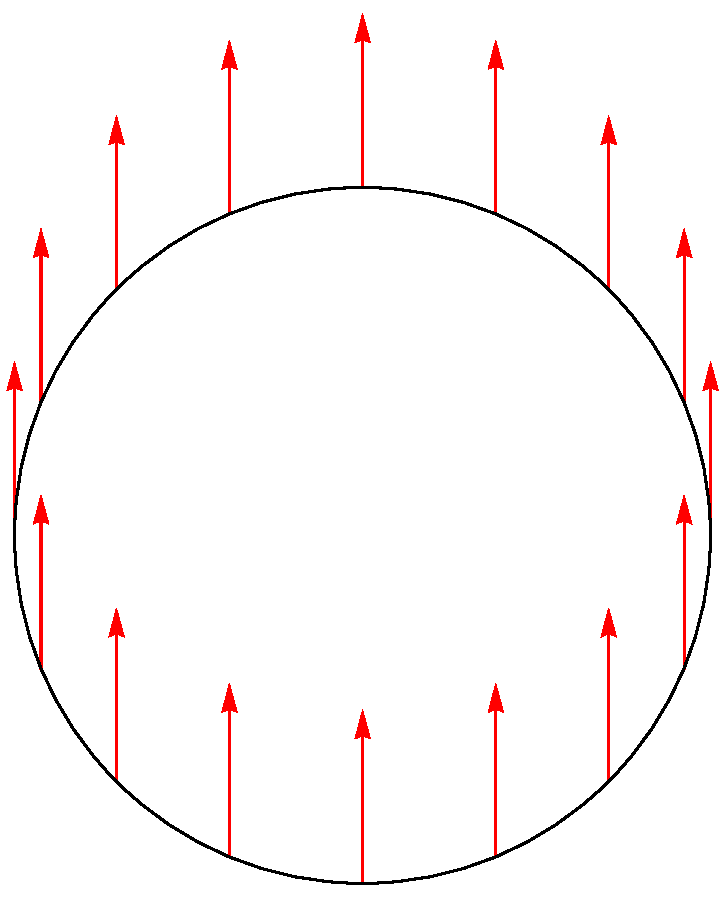
\includegraphics[scale=0.17]{lrg_gauge1.pdf} \text{(a)}  &  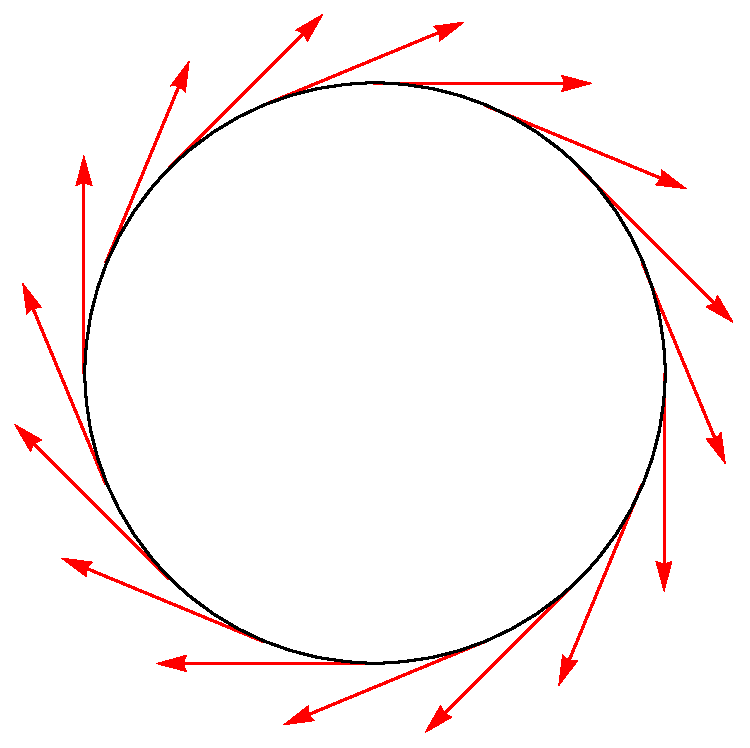
\includegraphics[scale=0.19]{lrg_gauge2.pdf} \text{(b)}  &
		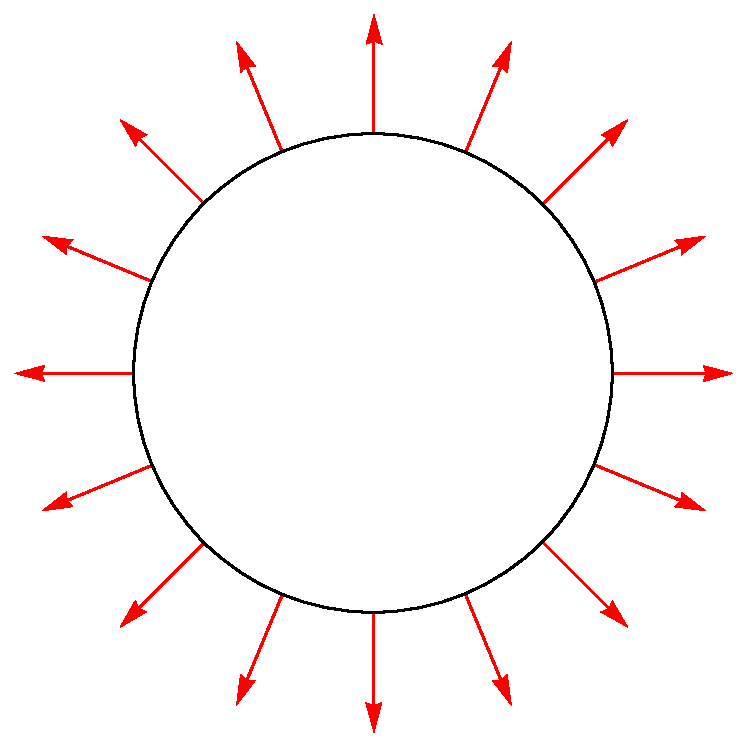
\includegraphics[scale=0.19]{lrg_gauge3.pdf} \text{(c)}
	\end{tabular}
    \caption[\textcolor{red}{This figure provides a simple example that illustrates the idea behind a large gauge transformation.}]{\textcolor{red}{This figure provides a simple example that illustrates the idea behind a large gauge transformation.} (a) is topologically distinct from the rest, yet they are all gauge equivalent configurations. } \label{large_gauge}
\end{figure}

As a final remark to counter the point that ``We don't live on a circle'', I shall say that when studying a non-singular circularly symmetric planar setup, we would require boundary conditions which identify the point at infinity with the same gauge-field configuration. It turns out that the point at infinity \textit{is} an $S^1$, so inevitably abelian gauge transformations \textit{would be} separated into distinct homotopy classes.

This above passage illustrates the essence of large gauge transformations in the simplest possible case, where we have a non-trivial homotopy group. The situation is precisely the same with more complicated homotopy groups but they just happen to be more difficult to visualize.

    Going back to the Lagrangian transformation law, we pick $g$, s.t. $w(g)=N$. Therefore \textcolor{red}{the action transforms as}
    \begin{align}
        S_{\text{CS}} \rightarrow S_{\text{CS } }+ 8 \pi^2 \kappa N.
    \end{align}
    Here we see that the action is \textit{not} gauge invariant! However, keep in mind that what plays a role in the path integral is $e^{i S}$, which transforms as
    \begin{align}
        e^{i S_{CS}} \rightarrow e^{i 8 \pi^2 \kappa N} e^{i S_{\text{CS}}}.
    \end{align}
    This implies that if we set $\kappa = \frac{k}{4 \pi}$, where $k\in \mathbb{Z}$, we have restored gauge invariance, which means that we ought to include this term in the study of planar physics.

    Let us look at some physical properties that the action functional $S_{\text{CS}} = \int d^3x \, \mathcal{L}_{\text{CS}}$ possesses. Performing the functional variation, we get the equation of motion $F_{\mu \nu}=0$, implying only pure gauge solutions exist. This might make one wonder, what could possibly be so interesting about CS theory if the classical equations of motion are trivial!?
    The reason that this theory is in fact interesting and non-trivial, despite the fact that $F=0$, is two-fold. Firstly, CS is a topological field theory. It has trivial local properties. All of the physics is encoded in the topology of the manifold and in the non-local observables such as Wilson loops that require us to study the full quantum theory.

    The second way in which CS is interesting teaches us the old lesson that sometimes the whole is greater than the sum of its parts. In this case, adding matter or a Maxwell term to the Lagrangian alters the pure Maxwell/matter theories immensely. Let us see how these alterations play out.

    \subsection{Chern-Simons-Maxwell Theory}
    Here we consider the familiar Maxwell theory deformed by a Chern-Simons term\colorbox{red}{ }
    \begin{align}
        \mathcal{L}_{\text{MCS}} &= \int d^3x \ \left[ \frac{-1}{4 g^2} F_{\mu \nu} F^{\mu \nu} + \frac{k}{4 \pi} \epsilon^{\mu \nu \rho} A_{\mu} \partial_{\nu} A_{\rho} \right]\colorbox{red}{.}
    \end{align}
    This leads to the equations of motion
    \begin{align}
        \partial_{\mu} F^{\mu \nu} + \frac{k}{4\pi} g^2 \epsilon^{\nu \alpha \beta}F_{\alpha \beta} =0\colorbox{red}{.}
    \end{align}
    If we rewrite this equation in terms of the dual field strength $\tilde{F}_{\mu} = \frac{1}{2} \epsilon_{\mu\nu\rho} F^{\nu\rho}$ by contracting with an $\epsilon$ tensor, followed by a $\partial$ contraction, using the equations of motion again and noting that $\partial_{\mu} \tilde{F}^{\mu} =0$ (3D Bianchi identity), we arrive at 
    \begin{align}
        \left[\partial_{\mu} \partial^{\mu} + \left(\frac{k}{2 \pi} g^2 \right)^2 \right] \tilde{F}^{\nu}=0.
    \end{align}
    Observing that $\tilde{F}^{\mu}$ is gauge-invariant, we deduce that these equations describe a propagating wave with mass $\left(\frac{k}{2 \pi} g^2 \right)$.
    Even though in this work we shall promptly be ignoring the Maxwell contribution to the planar physics, it is important to note that despite the fact that the gauge bosons are heavy, we still observe global effects. This provides us with a more general lesson about CS. Namely, that we can have significant long-rage global effects, such as the anyonic phase change interaction, even in the case of a gapped phase (such as the Quantum Hall droplet).
    Next, we turn to the matter sector.
    \subsection{Chern-Simons Matter Theory}
    
    We begin by coupling the Chern-Simons gauge field to a general conserved matter current\colorbox{red}{ }


    \begin{align}
        S = \int d^3x \ \frac{k}{4 \pi} \epsilon^{\mu \nu \rho} \ \mathrm{Tr} \left[A_{\mu} \partial_{\nu} A_{\rho}+ \frac{2}{3} A_{\mu} A_{\nu} A_{\rho} \right] + J^{\mu} A_{\mu}.
    \end{align}
    This action leads to a modified equation of motion\colorbox{red}{ }
    \begin{align}
        \frac{k}{4 \pi} \epsilon^{\mu \nu \rho} F^a_{\nu \rho} = J^{\mu}^a,
    \end{align}
    where $a=1,...,dim(\mathfrak{G})$ and $F_{\mu \nu}^a = \partial_{\mu} A_{\nu}^a - \partial_{\nu} A_{\mu}^a + [A_{\mu}, A_{\nu}]^a$. Note that covariant current conservation is equivalent to the non-abelian Bianchi identity
    \begin{align}
        D_{\mu} J^{\mu}^a = \frac{k}{4 \pi} \epsilon^{\mu \nu \rho} D_{\mu} F^{\nu \rho}^a = 0,
    \end{align}
    where $D_{\mu} F_{\nu \rho} = \partial_{\mu} F_{\nu \rho} + [A_{\mu}, F_{\nu \rho}]$.

    Restricting ourselves to the abelian case, we examine the equations of motion component by component. If $J_{\mu} = (\rho, J^i)$ then
    \begin{align}
        \rho  &= \frac{k}{4 \pi} B \label{eq:source_abel_charge} ,\\
        J^i &= \frac{k}{4 \pi} \epsilon^{i j } E_j \label{eq:source_abel_current},
    \end{align}
    where $B$ is the magnetic field perpendicular to the plane and $E_j$ is the electric field. The first equation \eqref{eq:source_abel_charge} relates the charge density to the magnetic field. So for a non-zero value of $k$, we find that anywhere there is charge, there is also magnetic flux penetrating through it perpendicular to the plane. This is something quite unlike Maxwell theory, where charge \textit{movement} generates a magnetic field, as opposed to charge \textit{presence}. This is illustrated in  Figure \ref{fig:flux_attachment} for a collection of localized charge distributions. The second equation \eqref{eq:source_abel_current} ensures that this charge-flux relation is preserved under time evolution. If we act with $\partial$ on \eqref{eq:source_abel_current} then we arrive at
    \begin{align}
        \partial_i J^i &= \frac{k}{4 \pi} \epsilon^{ij} \partial_i E_j\nonumber \\
        &= \frac{k}{4 \pi} \epsilon^{ij} \partial_i ( \partial_j A_0 - \partial_0 A_j) \nonumber \\
        &= -\frac{k}{4 \pi} \dot{B} = -\dot{\rho},
    \end{align}
    which is just the continuity equation $\dot{\rho} + \partial_i J^i=0$.





\begin{figure}[htb]
	\centering
		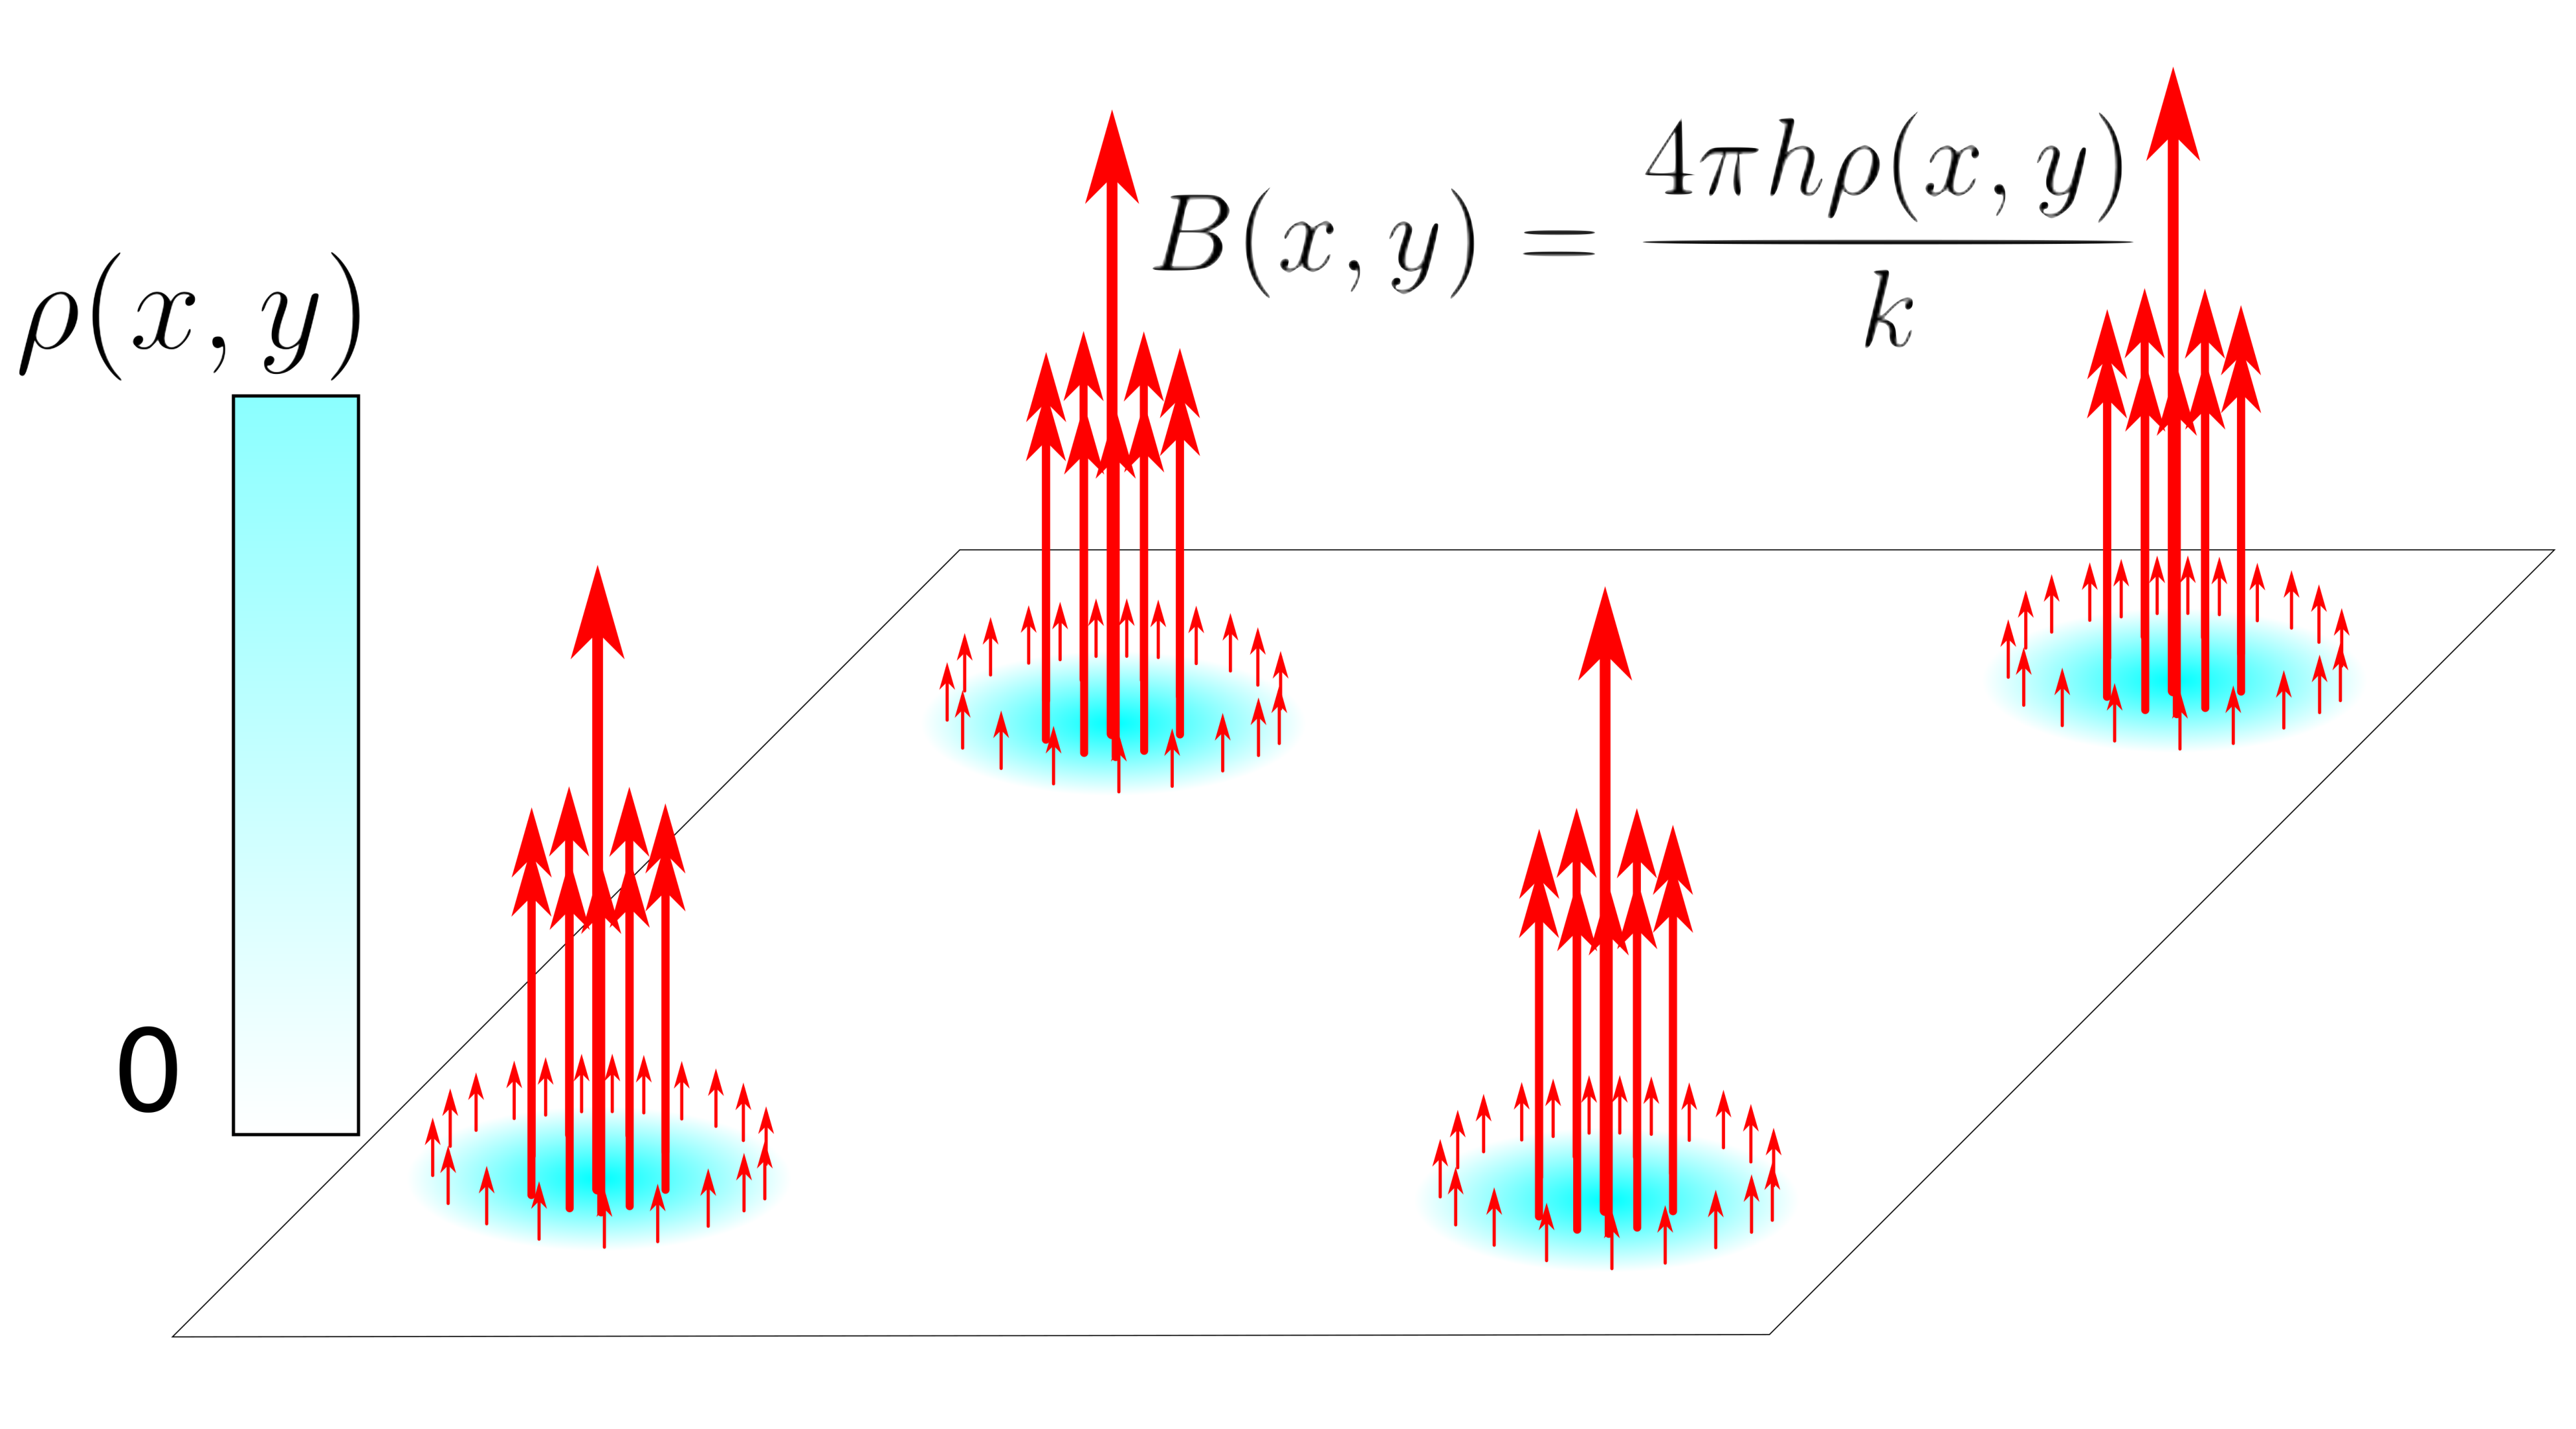
\includegraphics[scale=0.17]{Background_Folder/figures/flux_attachment_improved.pdf}
    \caption[\textcolor{red}{This figure depicts magnetic flux attachment.}]{A collection of localized charge distributions, and with magnetic flux lines of strength $\frac{4 \pi \hbar \rho(x,y)}{k}$ tied to the charges. \textcolor{red}{Here the charge density distribution is denoted by $\rho(x,y)$ and the magnetic field strength is denoted by $B(x,y)$. Darker shades of cyan depict a larger charge density and larger red vectors are associated with a stronger magnetic field perpendicular to the plane.}  The charge and flux are tied together throughout the motion of the particles as a result of the Chern-Simons equations \eqref{eq:source_abel_charge} - \eqref{eq:source_abel_current}.} \label{fig:flux_attachment}
\end{figure}

The final aspect of Chern-Simons theory that we will use is the fact that it is a \textit{topological} field theory (TQFT). This means that the theory is independent of the metric. This consequently implies that the CS term does not contribute to the energy-momentum tensor, since
\begin{align}
    T^{\mu \nu} = \frac{-2}{ \sqrt{-g}} \frac{\delta S_{\text{CS}}}{ \delta g_{\mu\nu}} =0.
\end{align}

One way to see that CS is a topological field theory is by writing it as an integral of a differential form\colorbox{red}{ }
\begin{align}
    S_{\text{CS}} &= \frac{k}{4 \pi} \int \left(A \wedge d \wedge A +A \wedge A \wedge A\right).
\end{align}
This construction does not require the metric to be defined, unlike the Yang-Mills term, which involves the hodge star (a metric dependent construct) in order to be defined through differential forms.

This concludes our review of CS theory. We now move on to a refresher of statistical physics.


        \section{Statistical Physics}

        Here we motivate the study of QFT as a gateway into understanding phenomena in many body physics. Physical phenomena at macro scale require micro scale explanations. The transition between a microscopic theory and its observable large scale properties is facillitated by the use of techniques in statistical mechanics. Here we review the connection between microscopic Lagrangian formulation and the statistical partition function through the formalism of the path integral. We follow through by accentuating the treatment of a chemical potential and the subtleties related to it. Before we go on, I note that this is the only part of this section that will be relevant to the calculations performed in this work. However, the rest of this section is meant to shine a light on why it is that we are interested in such an abstract problem.

        Upon completing this summary, we go through a short review of statistical mechanical paradigms, their successes and shortcomings. In particular, we will highlight how the Landau-Fermi liquid theory manages to do away with the complications arising from interactions and how succesful the Landau-Ginzburg symmetry breaking ideas have been in explaining large swathes of interesting phases of matter. 

        Finally, the failures of these extremely successful ideas will lead us to strongly correlated and topological systems. Notably, we discuss one system that seems to reject treatment from both of the above approaches -- a system of strongly interacting electrons confined to 2 dimensions, namely, the physical setup in which we observe the quantum hall effect. As the reader might suspect, the planar confinement is what forces us into considering CS theory as a natural candidate to explain the exotic properties of this structure.
        \subsection{Functional Integral Representation of the Partition Function}
        In this section we derive the functional integral representation of the partition function for interacting relativistic non-gauge field theories.
        Let $\hat{\phi}(\bm{x},0)$ be a Schr{\H o}dinger picture field operator at time $t=0$. We define its conjugate momentum operator to be $\hat{\pi}(\bm{x},0)$. The eigenstates of the field operator are labeled $| \phi \rangle$ and satisfy
        \begin{align}
            \hat{\phi}(\bm{x},0) | \phi \rangle = \phi(\bm{x}) | \phi \rangle,
        \end{align}
        where $\phi(\bm{x})$ is the eigenvalue of $| \phi \rangle$. This is complemented with the completeness and orthogonality relation
        \begin{align}
            \int d \phi(\bm{x}) | \phi \rangle \langle \phi | = 1, \\
            \langle \phi_a | \phi_b \rangle = \prod_{\bm{x}} \delta(\phi_a(\bm{x}) - \phi_b(\bm{x}))\colorbox{red}{.}
        \end{align}
        And similarly for the conjugate momentum
        \begin{align}
            \hat{\pi}(\bm{x},0) | \pi \rangle = \pi(\bm{x}) | \pi \rangle, \\
            \int d \pi(\bm{x}) | \pi \rangle \langle \pi | = 1, \\
            \langle \pi_a | \pi_b \rangle = \prod_{\bm{x}} \delta(\pi_a(\bm{x}) - \pi_b(\bm{x}))\colorbox{red}{.}
        \end{align}
        Suppose we have a Hamiltonian with no explicit time dependence
        \begin{align}
            H = \int d^2x \, \mathcal{H}(\hat{\phi}, \hat{\pi}).
        \end{align}
        Assume that a system is in a state $| \phi_a \rangle$ at time $t=0$. After a time $t_f$ it evolves to $e^{-i H t_f} | \phi_a \rangle$, assuming that the Hamiltonian has no explicit time dependence. The transition amplitude for going from state $| \phi_a \rangle$ to state $| \phi_b \rangle$ after a time $t_f$ is $\langle \phi_b | e^{-i H t_f} | \phi_a \rangle$. In order to study a system at thermodynamic equilibrium, we will be interested in the amplitude for the system returning to the same state after a time $t_f$. To be able to compute this amplitude, we divide the time interval $(0, t_f)$ into $N$ equal time steps $\Delta t = \frac{t_f}{N}$. Then at each time interval, we insert a complete set of states, alternating between field operators and their conjugate momenta


        \begin{align}
            \langle \phi_a| e^{- i H t_f} | \phi_a \rangle &= \lim_{N\rightarrow \infty} \int \left( \prod_{i=1}^{N} \frac{d\pi_i d\phi_i}{2\pi} \right) \nonumber \\
            &\times \langle \phi_a | \pi_N \rangle \langle \pi_N|  e^{-i H \Delta t}| \phi_N \rangle \langle \phi_N | \pi_{N-1} \rangle \nonumber \\
            &\times \langle \pi_{N-1} | e^{-i H \Delta t} | \phi_{N-1} \rangle \dots \nonumber \\
            &\times \langle \phi_2 | \pi_1 \rangle \langle \pi_1 | e^{-i H \Delta t} | \phi_1 \rangle \langle \phi_1 |\phi_a \rangle.
        \end{align}
        In order to evaluate this expression, we need to do several things. First of all, from single particle QM, we know that 
        \begin{align}
            \langle x | p \rangle = e^{i p \cdot x}.
        \end{align}
        So an appropriate generalization for this inner product to field operators is 
        \begin{align}
            \langle \phi_{i+1}| \pi_i \rangle = \exp \left(i \int d^2 x \ \pi_i(\bm{x}) \phi_{i+1}(\bm{x}) \right)\colorbox{red}{.}
        \end{align}
        Since $\Delta t \rightarrow 0$, we can expand as follows, keeping terms up to first order:
        \begin{align}
            \langle \pi_i | e^{-i H_i \Delta t} | \phi_i \rangle &\sim \langle \pi_i | (1- i H_i \Delta t ) | \phi_i \rangle \nonumber \\
            &= \langle \pi_i | \phi_i \rangle (1 - i H_i \Delta t) \nonumber \\
            & = (1-i H_i \Delta t) \ \exp\left(-i \int d^2x \, \pi_i(\bm{x}) \phi_i (\bm{x})  \right),
        \end{align}
        where
        \begin{align}
            H_i = \int d^2 x \ \mathcal{H}\left(\pi_i (\bm{x}) \phi_i (\bm{x}) \right) \colorbox{red}{.}
        \end{align}
        In the end we arrive at 
        \begin{align}
            \langle \phi_a | e^{-i H t_f} | \phi_a \rangle &= \lim_{N\rightarrow \infty} \int \left( \prod_{i=1}^N \frac{d \pi_i d\phi_i}{2\pi} \right) \delta \left(\phi_1 -\phi_a \right) \nonumber \\
            &\times \exp \left(i \Delta t \sum_{j=1}^{N} \int d^2x \left[\frac{\pi_j (\phi_{j+1} -\phi_j)}{\Delta t} - \mathcal{H}(\pi_j, \phi_j) \right] \right).
        \end{align}
        And taking the continuum limit we arrive at the path integral representation of the partition function
        \begin{align}
            &\langle \phi_a | e^{-i H t_f} | \phi_a \rangle = \int \mathcal{D} \pi \int_{\phi(\bm{x},0) =\phi_a(\bm{x})}^{\phi(\bm{x}, t_f) = \phi_a(\bm{x})} \mathcal{D} \phi \nonumber \\
            &\times \exp \left[i \int_0^{t_f} dt \int d^2 x \left( \pi(\bm{x} ,t) \frac{\partial\phi(\bm{x}, t)}{ \partial t} - \mathcal{H}\left(\phi(\bm{x},t), \pi(\bm{x},t)\right) \right) \right] \label{eq:path_integral_amplitude}.
        \end{align}
        For a Hamiltonian that is quadratic in the canonical momenta, we can just complete the square, integrate out the momenta and arrive at the usual expression for a transition amplitude in terms of a path integral over $e^{i S}$. Since our purpose here is to illuminate the connection between the statistical partition function and the path integral, we shall perform a few more manipulations. 
        \subsection{Grand Canonical Ensemble} \label{GCE_sec}
        First, we note that the grand canonical partition function is defined as follows
        \begin{align}
            Z= \tr \left[e^{-\beta \left( H - \mu N \right)}\right],
        \end{align}
        where $\beta = \frac{1}{k_b T}$ and is the inverse temperature and $\mu$ is the \textit{chemical potential}, and $N$ is a particle number. In a QFT this particle number will be associated with a conserved charge that is discretized, which is the reason why it is associated to particle number. We can express the trace in the $\phi$ basis
        \begin{align}
            Z= \int d \phi_a \langle \phi_a | e^{-\beta \left( H - \mu N \right)} | \phi_a \rangle.
        \end{align}
        We see that this expression is very similar to \ref{eq:path_integral_amplitude}. In order to match the two expressions, we need to do three things. First, we set $t \rightarrow -i \tau$, such that $t_f \rightarrow -i \beta$. Then we shift the Hamiltonian density in order to account for the inclusion of a chemical potential
        \begin{align}
            \mathcal{H} \left(\phi(\bm{x},t),\pi (\bm{x},t) \right) \rightarrow \mathcal{H}\left(\phi(\bm{x},t),\pi (\bm{x},t) \right) - \mu \ \mathcal{N}\left(\phi(\bm{x},t),\pi (\bm{x},t) \right),
        \end{align}
        where $\mathcal{N}$ is a number density. Finally, we include the trace operation, which integrates over all possible boundary conditions. In the end we are left with
        \begin{align}
            Z &= \int \mathcal{D} \pi \int_{\text{periodic}} \mathcal{D} \phi \exp \left[ \int_0^{\beta} \int d^2x \left(\pi \frac{\partial \phi}{\partial t} - \mathcal{H}(\pi, \phi) + \mu \mathcal{N}(\pi, \phi) \right) \right] \label{eq:partition_function}.
        \end{align}
This is the path integral representation of the partition function of the grand canonical ensemble of a single real scalar field. This expression is readily generalizable to more fields by integrating over the extra fields and their respective conjugate momenta.

Here we shall make a few observations that will come in use frequently for the rest of this work. For the purposes of presentation, we will elaborate on these points in the context of a somewhat simpler model. This should not alarm the reader, because the properties we are discussing are more general and model independent. With this in mind, we consider the Lagrangian description of a complex relativistic scalar in $2+1d$ with a potential $U(\phi)$\colorbox{red}{ }
        \begin{align}
            \mathcal{L} = \left(\partial_{\mu}\phi^{*} \partial^{\mu} \phi  - U\big(|\phi|\big)\right).
        \end{align}
        This system possesses a global symmetry
        \begin{align}
            \phi \rightarrow e^{i \alpha} \phi, \qquad\qquad \phi^* \rightarrow e^{-i \alpha} \phi^*.
        \end{align}
        This leads to a conserved Noether current and consequently a conserved charge
        \begin{align}
            J_{0} &= -i \int d^2x \left( \pi \phi - \pi^{\dag}\phi^{\dag}\right),
        \end{align}
        where $\pi = \frac{\delta \mathcal{L}}{\delta ( \partial_0 \phi)}$ is the canonical momentum. Based on the assumption of identical particles with discrete charges, we postulate that $J_0 = \mathcal{N}$. Next, we perform the momentum integrals in \eqref{eq:partition_function}. Since now we have a complex field, we have to integrate over all of $\phi$, $\phi^{\dag}$, $\pi$ and $\pi^{\dag}$\colorbox{red}{ }
        \begin{align}
            Z &= \int \mathcal{D} \pi \mathcal{D} \pi^{\dag} \int_{\text{periodic}} \mathcal{D} \phi \mathcal{D} \phi^{\dag} \nonumber \\
            &\times \exp \left[ \int_0^{\beta} \int d^2x \left(\pi \frac{\partial \phi}{\partial t} +\pi^{\dag} \frac{\partial \phi^{\dag}}{\partial t} - \mathcal{H}(\pi, \pi^{\dag}, \phi, \phi^{\dag}) - i  \mu \left(\pi \phi - \pi^{\dag}\phi^{\dag} \right) \right] \label{eq:partition_function_complex_scalar} \nonumber \\
            &= \int \mathcal{D} \pi \mathcal{D} \pi^{\dag} \int_{\text{periodic}} \mathcal{D} \phi \mathcal{D} \phi^{\dag} \nonumber \\
            &\times \exp \left[ \int_0^{\beta} \int d^2x \left(\pi \left( \frac{\partial \phi}{\partial t} -i \mu \phi \right) +\pi^{\dag} \left( \frac{\partial \phi^{\dag}}{\partial t} +i \mu \phi^{\dag} \right) - \mathcal{H}(\pi, \pi^{\dag}, \phi, \phi^{\dag}) \right) \right]\colorbox{red}{.} \label{eq:partition_function_complex_scalar}
        \end{align}
        Performing the path integral leaves us with
        \begin{align}
            Z= \int_{\text{periodic}} \mathcal{D}\phi \mathcal{D}\phi^{\dag} \exp \left[\int_0^{\tau} d\tau \int d^2x \mathcal{L'} \right],
        \end{align}
        where $\mathcal{L'}$ is the same as $\mathcal{L}$ except for the time derivatives acting on $\phi$ now act as covariant derivatives in the presence of a constant background gauge field $A_0=\mu$, \ie
        \begin{align}
            \partial_0 \rightarrow \partial_0 -i \mu. \label{eq:chemical_potential_gauge_field}
        \end{align}
        This is a general result that we will be making use of numerous times.
        \subsubsection{Chemical Potential for a Local Symmetry}
        Now, let us see how this situation changes when we try to introduce a chemical potential for a gauged symmetry. First, we modify the Lagrangian $\mathcal{L}$ by gauging the $U(1)$ and adding a Maxwell term $-\frac{1}{4 g^2} F_{\mu \nu} F^{\mu \nu}$. For simplicity, let us assume that the potential has the monomial super-renormalizable form
        \begin{align}
            U\big(|\phi| \big) = \lambda |\phi|^4.
        \end{align}
        Therefore
        \begin{align}
            \mathcal{L} &=( D_{\mu} \phi)^* D^{\mu} \phi - \lambda |\phi|^4 - \frac{1}{4 g^2}F_{\mu \nu} F^{\mu \nu},
        \end{align}
        where $D_{\mu}= \partial_{\mu} - i A_{\mu}$. According to the rule \ref{eq:chemical_potential_gauge_field} that we established above,\colorbox{red}{ }
        \begin{align}
            \mathcal{L} \rightarrow \mathcal{L}'= \mathcal{L}\left(\phi,\ D_{\mu}' \phi,\ A_{\mu} \right),
        \end{align}
        where $D_{\mu}' = D_{\mu} - i \mu \delta_{\mu 0}$.
        Let us also express $\phi$ in terms of a modulus and a phase
        \begin{align}
            \phi(x) = \sigma(x) e^{i \alpha(x)}.
        \end{align}
        If we assume a homogenous, constant configuration, the equations of motion tell us that
        \begin{align}
            \sigma &= \sqrt{\frac{\mu^2}{2\lambda}}  \label{eq:chem_pot_local_symmetry_eom1}\colorbox{red}{,} \\
            \frac{1}{g^2} \partial_{\mu} F^{\mu 0} &= \mu \sigma^2. \label{eq:chem_pot_local_symmetry_eom2}
        \end{align}
        The first equation tells us that the scalars have condensed to the ground state. The second equation states that we have a non-zero charge density in this ground state. On the one hand, this makes sense, since the charged scalars have condensed. On the other hand, this is contradictory, since we are studying a system at equilibrium. And a charged system cannot be in equilibrium by definition. In order to fix this problem, we introduce a background charge density, which guarantees that the system is neutral \colorbox{red}{ }
        \begin{align}
            \mathcal{L}' \rightarrow \mathcal{L}' - A_0 J_0,
        \end{align}
        where $J_0 = \frac{\mu^3}{2\lambda}$.

        %\subsection{Physical Applications}\label{phys_app_sec}
        %\subsubsection{Landau-Fermi Liquid Theory} \label{Fermi_Liquid_sec}
        The statistical description of weakly interacting particles, for example, in a fluid can be thought of as the same as that of a free gas of non-interacting quasiparticles that are in one to one correspondence with the original interacting excitations of the material. We find that in order to explain some of the surprising feature of the charge carriers in a QH system, we need to go beyond the weakly interacting description of a Landau-Fermi liquid.
        %\subsubsection{Landau-Ginzburg Paradigm} \label{Landau-Ginzburg_sec}
        %\textcolor{red}{***More to add***} \\
        %- Introductory part talk about the problem of scales, how mean field theory tackles the problems well away from the critical temperature, but at the critical point, all scales need to be taken into account. We are left with a LG functional that no longer contains information about the microscopic system -- we find a universal effective theory describing said phenomenon.
        %- Symmetry breaking \\
        %- Order parameters\\
        %- The Girvin MacDonald ``Landau-Ginzburg''-like model. \cite{Girvin1987} In 1987, Girvin \& MacDonald proposed a LG effective model to describe the FQHE. \\
        %- Read's improvement \cite{Read1989}\\
        %- The Zhang, Hansson, Kivelson microscopic Hamiltonian improvement \cite{PhysRevLett.62.82}
        \section{Fractional Quantum Hall Effect} \label{FQHE_sec}
        Here we discuss what is perhaps the most applied aspect of TQFT in the real world. But before we get to the point of discussing the highly non-trivial physics of the various types of Quantum Hall Effects, we take a moment to review the classical picture.
        \subsection{Classical Hall Effect}
        In the year 1879, Edwin Hall set up an experiment consisting of a conductor plate with two electrodes attached at either end of it, generating a current, and a magnetic field penetrating the surface of the conductor perpendicularly. He found that he could measure a non-zero potential across the conductor, orthogonal to the plane defined by the driving current and the magnetic field. The generation of this potential difference has since been known as the \textit{Hall effect}. Despite this being an exciting discovery at the time, from our modern perspective this is all accounted by basic knowledge of conductors and classical electrodynamics. In the presence of a magnetic field, the charge carriers, which are responsible for the current in the conductor, get deflected in a direction orthogonal to their motion due to the Lorentz force
        \begin{align}
            F = q(\bm{E} + \bm{v}\times \bm{B}),
        \end{align}
        where $q$ is the charge of the electrons, $\bm{E}$ is the electric field due to the potential difference in the electrodes, $\bm{v}$ is the velocity of the charge carriers and $\bm{B}$ is the magnetic field in the material. If we were to account for the possible collisions that may occur within a sample of the conductor, which will cause the charge carriers (in this case electrons) to slow down, we shall arrive at a slightly modified equation to the Lorentz law from above
        \begin{align}
            m \dot{\bm{v}} = q \bm{E}+q \bm{v}\times \bm{B} - \frac{1}{\tau} m \bm{v}, \label{eq:Drude_Model_Background}
        \end{align}
        where $\tau$ is the \textit{scattering time} -- it accounts for how frequently the electrons scatter, hence a large scattering time makes the term disappear completely. This description of the charge carriers in a material, subject to both electric and magnetic field, in the presence of impurities, is called the \textit{Drude model}, named after the German physicist Paul Drude, who first proposed it. Before we look at the general solution of this model, we make several remarks about certain limiting cases.\\
        \indent First, assume that there are no collisions (\textit{i.e.} the collision time diverges $\tau \rightarrow\infty$) and that there is no electric field. Then the system simplifies to
        \begin{align}
            m\dot{\bm{v}} =q \bm{v}\times \bm{B}.
        \end{align}
        For a particle confined to the plane the velocity vector is $\bm{v} = (\dot{x}, \dot{y})$, which leads to the system of two coupled linear ODEs
        \begin{align}
            m \ddot{x} = q B \dot{y}, \qquad m \ddot{y}= -q B \dot{x}.
        \end{align}
        The general solution to this system is
        \begin{align}
            x(t) &= x_0 + R \sin\left(\omega_Bt + \varphi \right)\colorbox{red}{,} \\
            y(t) &= y_0 + R \cos\left(\omega_Bt + \varphi \right),
        \end{align}
        where $x_0, y_0, R, \varphi$ are all integration constants and
        \begin{align}
            \omega_B = \frac{q B}{m}
        \end{align}
        is the \textit{cyclotron frequency}.
        We that the solution in the absence of collisions and an electric potential is circular motion with a fixed magnetic field dependent frequency.\\
        Let us go back to the full Drude model. We would like to find out what the equilibrium of the system looks like. This implies that $\dot{v} =0$. The equation of motion becomes 
        \begin{align}
            \bm{v} - \frac{q \tau}{m}\bm{v}\times\bm{B}  &=\frac{\tau q}{m} \bm{E} \colorbox{red}{,}\\
            \begin{bmatrix}
                1 & -\frac{q \tau B}{m} \\
                \frac{q \tau B}{m} & 1 \\
            \end{bmatrix} \bm{v} &= \frac{\tau q}{m} \bm{E}.
        \end{align}
        Subsituting $\bm{J} = q \bm{v}$ and $\omega_B = \frac{q B}{m}$
        \begin{align}
            \begin{bmatrix}
                1 & -\omega_B \tau \\
                \omega_B \tau & 1 \\
            \end{bmatrix}\bm{J} = \frac{\tau q^2}{m} \bm{E}.
        \end{align}
        After inverting we arrive at \textit{Ohm's law}
        \begin{align}
            \bm{J}=\sigma \bm{E},
        \end{align}
        where
        \begin{align}
            \sigma=\frac{q^2 \tau }{m \left(\tau ^2 \omega_B ^2+1\right)}
\begin{bmatrix}
 1 & \tau  \omega_B  \\
 -\tau  \omega_B  & 1 \\
\end{bmatrix}
        \end{align}
         is the \textit{conductivity} tensor. It is related to the \textit{resistivity} tensor by
         \begin{align}
            \rho = \sigma^{-1}= \frac{m}{q^2 \tau } \begin{bmatrix}
 1 & -\tau  \omega_B  \\
 \tau  \omega_B  & 1 \\
            \end{bmatrix} = \begin{bmatrix}
                \rho_{xx} & \rho_{xy} \\
                \rho_{yx} & \rho_{yy} \\
            \end{bmatrix},
         \end{align}
         where $\rho_{xx} =\rho_{yy}$ and $\rho_{xy} = - \rho_{yx}$.

         This equation tells us that in the presence of a constant magnetic field, the charge carriers experience two types of resistivity. One is the usual type of resistivity that you can expect from a conductor $\rho_{xx} = \frac{m}{q^2\tau}$ -- It is independent of the magnetic field and as the scattering time increases, \textit{i.e.} the number of scattering events decreases, the resistivity decreases. The other type of resistivity is different. The off-diagonal component of the resistivity $\rho_{yx} = \frac{m \omega_B}{q^2}= \frac{B}{q}$ is independent of $\tau$. So somehow the resistivity in the direction orthogonal to that of the driving current does not depend on the impurities in the material. Another way in which $\rho_{yx}$ is different is that it depends on the magnetic field. Surprisingly, as $B\rightarrow 0$ so does $\rho_{yx} \rightarrow 0$. It would be incorrect to assume that the vanishing of $\rho_{xy}$ implies that we achieve superconductivity, since $\sigma_{xy}$ also vanishes so there is no current being generated perpendicular to the generating electric field.

        The Drude model is successful when compared to the classical experimental results obtained by Hall since it predicts correctly that the resistivity  $\rho_{xy}$ would grow linearly with the magnetic field $B$.
        \subsection{Quantum Hall Effect}
        Now that we have an understanding of the classical Hall effect we are ready to delve into the physics of the quantum hall effect. It's important to distinguish two different types of quantum Hall effects, since they are qualitatively different, occur in different materials and seem to have fundamentally different physical explanations.
        The first type is the Integer Quantum Hall effect. In 1980, Klaus von Klitzing was performing the Hall experiment at ultralow temperatures with strong magnetic fields and found that the above relation between $\rho_{yx}$ and $B$ does not hold for large enough magnetic fields. He found that beyond a certain magnetic field strength, plateaux started appearing in the resistivity that could not be explained by the classical picture. Further, he found that in the plateaux, where $\rho_{yx}$ was constant, $\rho_{xx}$ was vanishing. The precise relation that he discovered was
        \begin{align}
            \rho_{yx} = \frac{2 \pi \hbar}{e^2} \frac{1}{\nu}, \qquad \nu \in \mathbb{Z}.
        \end{align}
        Thus the quantity $\frac{2 \pi \hbar}{e^2}$ is dubbed the quantum of resistivity. The explanation of the Integer Quantum Hall effect is based on the quantum mechanics of non-interacting particles confined to a plane. In the case of the fractional quantum hall effect (FQHE), where $\nu \in \mathbb{Q}$, we need to study a highly interacting system, which makes the FQHE a very interesting topic for theoretical physics.

        Our exploration of the Quantum Hall Effect will stop here. What is important to take away from this section is that the understanding of the FQHE is underlied by the study of Chern-Simons theory. Thus studying the models, that are of interest in the present work, might lead to a better understanding of the fascinating problem that is the FQHE. A further connection to this problem is provided by the non-commutative Chern-Simons theory that we explore at the end of this chapter and at the end of chapter 3. Next, we turn our attention to the study of vortices.

%\textcolor{red}{***More to add***}\\
%        - Drude Model
%        - Classical electrodynamic explanation of classical Hall effect\\
%        - Integer Quantum Hall effect \\
%   \indent         - discovered by von Klitzing\\
%        - Fractional Quantum Hall effect\\
%    \indent        - Leads to charge fractionalization\\
%           \indent - Laughlin wave function
        \section{Vortices} \label{vortices_sec}
        This section takes up the task of summarizing basic aspects about vortices in general and specifically in Chern-Simons matter theories.
        Vortices are localized, exact solutions to the equations of motion. They may or may not be finite energy configurations.
        In 1957, Abrikosov  showed that if the surface tension between two phases of matter (in his case those were superconducting and non-superconducting phases) is negative, then a phase transition would be accompanied by the creation of a lattice of regions, whose interiors reside in a phase different from their exteriors \cite{Abrikosov1957}. He also recognized the similarity between these regions of non-superconductivity have with the vortices formed in superfluid helium. This similarity is due to the winding of the phase of the order parameter wave function.


        Later on, in 1973, Nielsen \& Olesen \cite{Nielsen1973} showed that a solution similar to that of Abrikosov can come about through the study of a microscopic Lagrangian, as opposed to in an effective Landau-Ginzburg description. This is the Lagrangian of the abelian Higgs model with a quartic interaction. Similar solutions have been found in the abelian Higgs model with a Chern-Simons interaction by Paul-Khare \cite{Paul1986} and in the absence of a Maxwell term by Hong-Kim-Pac \cite{Hong1990}, Jackiw and Weinberg \cite{Jackiw1990a} and Jackiw, Lee and Weinberg \cite{Jackiw1990b}.

        \subsection{Global U(1) Vortex}

        Now we look at the properties of these solutions more closely. Before we look at the gauge theory scenario, we focus on the simplest case of a complex massive scalar with a fourth order interaction, negative mass squared and a global $U(1)$ symmetry

        \begin{align}
            \mathcal{L} &=  \left|\partial_{\mu} \phi \right|^2 + m^2 | \phi |^2 - \lambda |\phi|^4.
        \end{align}
    This leads to the equations of motion
    \begin{align}
        \partial_{\mu} \partial^{\mu} \phi = m^2 \phi - 2\lambda |\phi|^2 \phi\colorbox{red}{.}
    \end{align}
    This system has an $S^1$ vacuum manifold, parametrized by $\phi = v e^{i \theta}$, where $\theta \in [0,2\pi)$ is the planar polar angular coordinate and $v^2 = \frac{m^2}{2 \lambda}$. We may consider a field configuration that is $\phi=0$ at the origin but approaches a different point on the vacuum manifold at spatial infinity depending on $\theta$. More precisely, we are looking at a field $\phi$ such that
    \begin{align}
        \phi \xrightarrow[]{r\rightarrow \infty} v e^{i n\theta},
    \end{align}
    where $n \in \mathbb{Z}$ in order to guarantee that the physical configuration is single-valued.
    We would like to compute the energy of such a static circularly symmetric configuration

    \begin{align}
        E= 2 \pi \int_0^{\infty} r dr \left[\lambda |\phi|^4 - m^2 |\phi|^2 + |\phi'|^2 + \frac{n^2 v^2}{r^2} \right].
    \end{align}
    Close to infinity, the potential term vanishes and so does $\phi'$. In the end we are left with
    \begin{align}
        E = 2\pi n^2 v^2 \int \frac{dr}{r} =  2\pi n^2 v^2  \ \log R,
    \end{align}
    where $R$ is the sample size on which our theory is defined. We see that the global vortex, if it exists, would only have a finite energy for finite samples and is not well-defined in the most general case. It turns out that once the global symmetry is gauged, the divergence disappears and we have a vortex configurations that is well defined in the infinite volume limit.

        \subsection{Local U(1) Vortex}
        The gauged $U(1)$ vortex, also known as the Abrikosov-Nielsen-Olesen vortex is again a configuration that interpolates between two different vacua in a theory, but this time we introduce a gauge field, whose dynamics is governed by a Maxwell term and is minimally coupled to a $U(1)$ scalar with a symmetry breaking potential. This is the familiar abelian Higgs model\colorbox{red}{ }
        \begin{align}
            S_{\text{AH}} & = \int d^3x \left[-\frac{1}{4} F_{\mu \nu} F^{\mu \nu} + | D_{\mu} \phi|^2 - U(\phi) \right], \label{eq:Abelian_Higgs_Model}
        \end{align}
        where
        \begin{align}
            U(\phi) = \frac{\lambda}{2} |\phi|^4 - m^2 |\phi|^2.
        \end{align}
    Again, we have non-trivial manifold of ground states and we can repeat the construction from above. This time the energy of the static radially symmetric configuration ends up slightly different\colorbox{red}{ }
    \begin{align}
        E = 2 \pi \int_0^{\infty} r dr \left(\frac{1}{2}( B^2 + E^2) + |D_{\mu} \phi|^2 + U(\phi) \right) \colorbox{red}{.}
    \end{align}
    This time we are aiming for eliminating the divergence that arose from the kinetic term $|\partial_{\mu}\phi|$ by requiring that $A_{\mu}$ asymptotes to a value that cancels it, in such a way that this value can be arrived at through a gauge transformation, ensuring that at $r\rightarrow \infty$, $A_{\mu}$ is pure gauge, thus yielding a finite contribution from the electromagnetic field. Such a choice for $A_{\mu}$ is
    \begin{align}
        A_{\mu} = n \partial_{\mu} \alpha(x),
    \end{align}
    where $\alpha(x) = \theta$. Hence
    \begin{align}
        A_0 =0, \qquad A_r =0, \qquad A_{\theta} = n.
    \end{align}
    This implies that
    \begin{align}
        \int_0^{\infty} r dr |D_{\mu}\phi|^2 = v^2\int_0^{\infty} r dr  \frac{1}{r^2}|n-A_{\theta}|^2 =0.
    \end{align}
    From here we see that the inclusion of a gauge field has cured the divergence and we are left with a sensible infinite volume limit. 

    Now that we know that these boundary conditions do not lead to a divergence in the energy, let us see whether a solution with such boundary conditions exists. We write down the equations of motion\colorbox{red}{ }
    \begin{align}
        \frac{1}{g^2}  \partial_{\rho}(r F^{\mu \rho}) = i r \left[\phi^* \left(D^{\mu}\phi\right) - \left(D^{\mu}\phi \right)^* \phi \right]\colorbox{red}{,} \nonumber \\
        \partial_{\mu} \left(r D^{\mu} \phi \right) - i A_{\mu} D^{\mu} \phi + \frac{\delta U}{\delta \phi^*} =0\colorbox{red}{.}
    \end{align}
    After substituting the ansatz
    \begin{align}
        \phi = \sqrt{\frac{m^2}{\lambda}}v(r) e^{i n \theta}, \qquad A_{\mu} = n a(r) \delta_{\theta \mu},
    \end{align}
    and rescaling $r\rightarrow \frac{\hat{r}}{m}$, we arrive at a system of equations for the dimensionless functions $v(r)$ and $a(r)$\colorbox{red}{ }
    \begin{align}
        \frac{1}{\hat{r}} \frac{d }{d \hat{r}} \left(\hat{r} \frac{d v}{d \hat{r}} \right) - \frac{n^2 (a-1)^2 v}{\hat{r}^2} -v^3 +v =0\colorbox{red}{,}  \\
        \frac{d}{d \hat{r}}\left(\frac{1}{\hat{r}}\frac{d}{d \hat{r}} a \right)- \frac{2 g^2}{\lambda r} (a-1)v^2=0.
    \end{align}
    In these variables, the boundary conditions become
    \begin{align}
        v(0) = 0, \qquad a(0)=0, \\
        v(\infty) =1, \qquad a(\infty) =1.
    \end{align}
    For small $r$, the solutions to these equations look like
    \begin{align}
        v(r)&= J_n(r) \sim \frac{r^n}{ 2^n n!}\colorbox{red}{,} \\
        a(r)&= C r^2\colorbox{red}{.}
    \end{align}
    And asymptotically for large $r$ we have
    \begin{align}
        v(r)&=K_0\left(\sqrt{2} r\right)\sim 2^{-\frac{3}{4}}\sqrt{\frac{\pi}{r}} e^{- \sqrt{2} r} \colorbox{red}{,} \label{eq:Asymptotics1_Abelian_Higgs} \\
        a(r)&=r K_1\left(\frac{\sqrt{2} g}{\sqrt{\lambda}} r \right)\sim 2^{- \frac{3}{4}} \sqrt{\frac{\pi r \sqrt{\lambda}}{g}} e^{- \sqrt{2} \frac{g}{\sqrt{\lambda}}r}\colorbox{red}{.} \label{eq:Asymptotics2_Abelian_Higgs}
    \end{align}
    \colorbox{red}{The system is solved numerically and plotted in Figure \ref{fig:Abelian_Higgs_Profiles_n1} below.}
\begin{figure}[htb]
	\centering
	\begin{tabular}{c@{\hspace{1.5cm}}c@{\hspace{1.5cm}}c}
        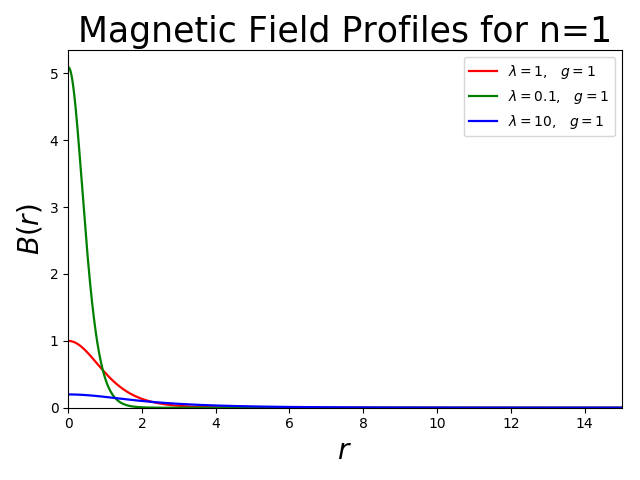
\includegraphics[scale=0.4]{Background_Folder/figures/solution_n1_magnetic_field_g_lambda.png}
        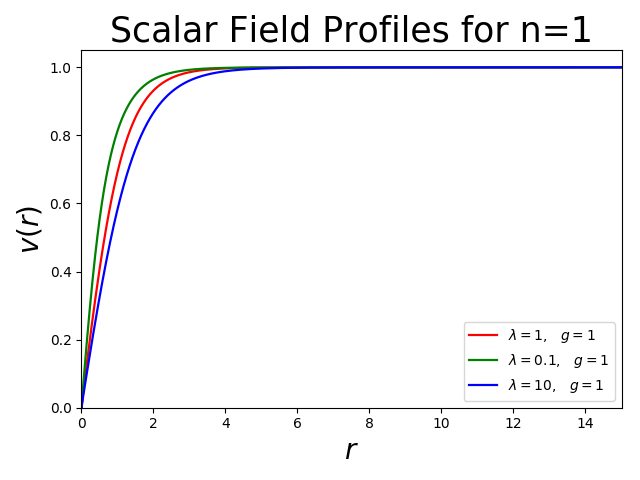
\includegraphics[scale=0.4]{Background_Folder/figures/solution_n1_scalar_field_g_lambda.png}
	\end{tabular}
    \caption[\textcolor{red}{This figure depicts the magnetic and scalar field profiles in the Abelian Higgs model.}]{\textcolor{red}{The profiles for the magnetic (left) and scalar (right) fields ($B(r)$ and $v(r)$, respectively) are depicted} for \textcolor{red}{winding number} $n=1$\textcolor{red}{, electromagnetic coupling $g=1$} and \textcolor{red}{quartic interaction coupling} $\lambda = (10,1,0.1)* \lambda_c$. \textcolor{red}{Here, $\lambda_c$ is the critical coupling, for which the BPS equations \eqref{eq:BPS1_Abel} hold.}} \label{fig:Abelian_Higgs_Profiles_n1}
\end{figure}

    From \textcolor{red}{the asymptotic equations \eqref{eq:Asymptotics1_Abelian_Higgs} and \eqref{eq:Asymptotics2_Abelian_Higgs},} we can recover the masses of the \textcolor{red}{Higgs} field and \textcolor{red}{gauge} field $m_{H}$ and $m_a$, respectively, in the Higgsed phase of the theory\colorbox{red}{ } 
    \begin{align}
        m_{H}= \sqrt{2} m, \qquad m_a = \sqrt{2} \frac{g^2}{\lambda}m \colorbox{red}{.}
    \end{align}
    From the from of the propagator for scalar and vector theories, we know that scalar fields act attractively, whereas gauge fields act repulsively for like-charged configurations. This tells us that when $m_a>m_H$, the \colorbox{red}{scalar} field decays slower than the \colorbox{red}{gauge} field, so if we were to place two vortices on the plane, we will observe an attractive force between them. Likewise, if  $m_a<m_H$, we expect the vortices to repel each other. This line of thought hints at us that there is a critical value of the couplings, where vortices are free (non-interacting). Here we present a more precise argument for this. In order to do this, we will Bogomol'nyi's identity\colorbox{red}{ }

    \begin{align}
        |D_1 \phi|^2 + |D_2 \phi|^2 = |D_1 \phi \pm D_2 \phi|^2 \pm B |\phi|^2. \label{eq:Bogomolnyi}
    \end{align}
    Further, we re-express the potential by completing the square\colorbox{red}{ }

    \begin{align}
        U(\phi)&=\frac{\lambda}{2} \left( |\phi|^2 - v^2 \right)^2 - \frac{m^2 v^2}{2}. \label{eq:potential_square}
    \end{align}
    Here we can ignore the constant since the energy is defined up to a constant (albeit an infinite one). Utilizing \eqref{eq:Bogomolnyi} and \eqref{eq:potential_square} we reach the following expression for the energy of this configuration

    \begin{align}
        E &= 2 \pi \int r dr \bigg(\frac{1}{2 g^2}B^2 \pm B(|\phi|^2 -v^2) + \frac{\lambda}{2} \left(|\phi|^2 -v^2 \right)^2 \\ \nonumber 
        &+ |D_1\phi \pm i D_2 \phi|^2 \pm B v^2 \bigg) \\ \nonumber
        &= 2 \pi \int r dr \bigg[|D_1\phi \pm i D_2 \phi|^2 +\frac{1}{2}\left( \frac{B}{g} \pm \lambda \left(|\phi|^2 -v^2  \right) \right)^2   \\ \nonumber \\
        &\pm \left(1 - \frac{\sqrt{\lambda}}{g} \right) B \left(|\phi|^2 - v^2 \right) \bigg] \pm n v^2,
    \end{align}
    where we have used Stokes' theorem.

    \begin{align}
        \int r dr B = n.
    \end{align}

    In order to have no interaction between the vortices, we need the energy of the $n$ vortex, the bound state of n vortices, to be the same as the energy of $n$ separate vortices. This implies that there is no potential energy, hence no force between them. This condition is satisfied when

    \begin{align}
        |D_1\phi \pm i D_2 \phi|^2 =0&,  \qquad \frac{B}{g} \pm \lambda \left(|\phi|^2 -v^2  \right) =0, \label{eq:BPS1_Abel}\\
        \lambda &= g^2 .\label{eq:BPS2_Abel}
    \end{align}
    The above equations (\eqref{eq:BPS1_Abel} and \eqref{eq:BPS2_Abel}) are known as the BPS equations of the vortex, named after the people who first discovered a non-interacting limit for solitonic solutions in field theory -- Bogomol'nyi, Prasad and Sommerfield \cite{Bogomolny:1975de} \cite{Prasad1975}.
    

    \subsection{Particle-Vortex Duality}
    The considerations of the previous section are more general and they apply for more than just systems in $2+1d$ even though the details differ. In a general QFT, we have roughly two different types of quantum excitations. One is the familiar type of elementary excitations that appear through the standard procedure of canonical quantization, where we introduce creation and annihilation operators that insert particles at a given position. The other type is, as we have just seen from the previous section, of a \textit{solitonic nature} (such as vortices). In other words, a solution that we reach not through expanding around the free solution in a small coupling parameter, but is more generally associated with a stationary point parametrically far from the free theory. This makes these solutions grow in size and energy the smaller the coupling is so studying them in the quantum regime becomes tricky. Luckily, because their masses become large at small coupling, they decouple from the theory so one can study the quantum theory of the elementary excitations on its own without worrying about the solitons. Unfortunately, going in the other direction in terms of coupling strength, the solitons become light and their importance grows but so do quantum corrections for the elementary excitations and we reach a regime, where we do not understand the theory. So how do we learn more about these strongly coupled theories?

    One approach that has become ever more popular in the past few decades is the idea of a \textit{duality}. Duality suggests that instead of having one model or one Lagrangian that describes the physics of a system, we instead have two. For example, a way in which duality can manifest itself is the following. Theory \textit{I} has elementary excitations that we can study at weak coupling and non-perturbative excitations which are inaccessible due their large mass. Whereas theory \textit{II} describes the solitons of theory \textit{I} as its own elementary excitations at weak coupling (and a small mass) and the solitons present in theory \textit{II} are in fact the elementary states of theory \textit{I}. If the non-perturbative states in these systems are vortices in $2+1$ dimensions, then we have a type of Strong-Weak duality called a \textit{Particle-Vortex duality}. 

    Since we now have a reasonable grasp of what vortices are, we are ready to introduce particle-vortex duality. And what better place to start than the Abelian Higgs model from the last section \eqref{eq:Abelian_Higgs_Model}. Earlier we saw that non-perturbative solutions exist in this theory. It turns out that a model exists where the vortices of the Abelian Higgs model appear as elementary excitations. In other words, there is a duality between these two models
    \begin{align}
        S_{\text{AH}} \longleftrightarrow S_{\text{XY}},
    \end{align}
    where
    \begin{align}
        S_{\text{XY}} &= \int d^3x |\partial_{\mu}\tilde{\phi}|^2-m^2 |\tilde{\phi}|^2 - \frac{\tilde{\lambda}}{2} |\tilde{\phi}|^4.
    \end{align}
    $S_{\text{XY}}$ is the action for the so called \textit{XY model} and $S_{\text{AH}}$ is defined as in \eqref{eq:Abelian_Higgs_Model}. The matching of the physics in the different phases is summarized in table \eqref{table:PV_Duality}.

    \begin{table}
\begin{center}
  \begin{tabular}{| l | c | c | c|}
      \hline
    $m^2$ & $<0$ & $=0$ & $>0$\\ \hline
     & Coulomb phase &  & SB phase\\ 
    $S_{\text{XY}}$ & $2d$ logarithmic & WF fixed point & local ANO \\ 
     & potential &  & vortices \\ \hline
      & SB phase &  &  Massive excitations\\
    $S_{\text{AH}}$ & global vortices & WF fixed point & in\\
      & $E\xrightarrow{V \rightarrow \infty} \infty$ &  & Coulomb phase \\
    \hline
  \end{tabular}
\end{center}
      \caption{This table shows the matching of the phases of the XY model and the Abelian Higgs model}
        \label{table:PV_Duality}
    \end{table}
In \cite{1606.01893}, the authors showed a link between this particle-vortex duality and bosonization. This naturally leads us to the next section, which focuses on Fermi-Bose duality.


%\textcolor{red}{***More to add***}\\
%-- Say something about the relation between particle-vortex duality and bosonization \cite{1606.01893, 1606.01912} \\
%Some history, Abrikosov \cite{Abrikosov1957}, type $I$ and $II$ superconductors. Vortices are solitons -- this means that they are non-perturbative solutions to the equations of motion that are localized and stable.\\
%            - Topological vs Non-Topological\\
%            - Review other vortices such as Abrikosov, Abelian Higgs, Pure Chern-Simons, Non-abelian vortices
%

%    \begin{itemize}
%        \item Tong TASI Solitons \cite{hep-th/0509216}
%        \item Importance of BPS \cite{Bogomolny:1975de, Prasad1975}
%    \end{itemize}
        \section{Fermi-Bose Duality} \label{Fermi-Bose_sec}
        We already met the idea of duality in the previous section. In general, they tend to be an equivalence of two theories. Two different ways in which we can state the same physics. Some of them are functional integral analogs of the Fourier transform (for functionals) -- one phenomenon can be described either in coordinate or momentum space, by one action or another. This can be achieved by introducing a Lagrange multiplier field and integrating out the original fields. Others tend to arise in consequence of the idea of universality. Two models that flow to the same CFT in the IR will tend to be equivalent sufficiently close to the fixed point.
        Yet other types of duality are inspired by the study of black hole thermodynamics and the holographic principle, such as the AdS/CFT duality. Others still, seem to be a consequence of deep mathematical ideas, such as the level-rank duality.

        Whatever the fundamental reasons for their existence is, dualities are interesting becase they give us another point of view that allows us to explore and understand the world of fundamental physics in more depth. As Feynman once said, ``Every theoretical physicist who is any good knows six or seven different theoretical representations for exactly the same physics''\cite{Feynman_quote}. And in the spirit of his words, here duality is one more representation we wish to understand.\\
        \indent As pointed out above, dualities come in many flavours and the models we are considering here play a role in more than one type. $O(N)/U(N)$ (scalar or fermion) models are holographically dual to higher spin gravitational theories \cite{hep-th/0210114}. This duality seems to persist even after deforming the theories with a Chern-Simons term in the large $N$ limit\cite{1110.4382}. Fermions in 2+1d can be shown to be dual to vector fields via a Fourier transform-like functional integral transformation that we described above \cite{hep-th/9401105, Barci1996}. And pure Chern-Simons theories are level-rank dual to each other \cite{Naculich1990, Camperi1990, Mlawer1991, Nakanishi1992, hep-th/0703089}. In this section, we will concentrate on a duality that has all of the above ingredients in some form ($SU(N)/U(N)$ scalars/fermions and CS vector fields) that combine into what's believed to be an IR duality. More precisely, we are talking about a set of dualities between $2+1d$ gauge theories that are collectively known as \textit{Fermi-Bose duality}.\\
        \indent The duality between fermions and bosons was first conjectured  in the supersymmetric context\cite{0808.0360, 1108.5373, 1305.3924, 1411.5475}. Evidence for the non-supersymmetric version of these dualities comes from large $N$ computations on both sides both at finite temperature \cite{1211.4843}  and at $T=0$ \cite{1110.4386}. Furthermore, there is compelling evidence that the duality holds at finite $N$ from supersymmetric theories flowing to their non-SUSY versions \cite{1305.7235, 1507.04378}.\\
        \indent Since $U(N) = (SU(N)\times U(1))/\mathbb{Z}_N$, we can in principle have different Chern-Simons levels for the $SU(N)$ and $U(1)$ symmetries. We will denote a $U(N)$ Chern-Simons theory with levels $k_1$ and $k_2$ corresponding to the $SU(N)$ and $U(1)$ symmetries, respectively, as a $U(N)_{k_1,k_2}$ theory. Prior to the inclusion of matter in our model, we state an important fact about these theories. Namely, that some choices of gauge groups and levels are dual to others. This is known as \textit{level-rank duality}. It's generalization to include matter is the duality that we present below. In Yang-Mills regularization the Fermi-Bose dualities are as follows \cite{1512.00161} \colorbox{red}{ }
            \begin{align}
                SU(N)_k + scalars &\longleftrightarrow \ \ U(k)_{-N +\frac{N_f}{2}, -N + \frac{N_f}{2}} \quad + fermions,  \\
                U(N)_{k,k} + scalars &\longleftrightarrow SU(k)_{-N +\frac{N_f}{2}}\qquad \ \ \ \quad+ fermions,  \\
                U(N)_{k,k+N} + scalars &\longleftrightarrow \ \ U(k)_{-N +\frac{N_f}{2}, -N + \frac{N_f}{2}-k} \ + fermions.  
            \end{align}
            The scalars on the LHS of these equations are assumed to be tuned to a critical interacting point of the RG flow, known as the Wilson-Fisher fixed point. (Explain how the Wilson Fisher fixed point work). Similarly to PV duality, which maps elementary excitations to non-perturbative vortices, Fermi-Bose duality maps the fundamental perturbative states on one side to monopole or baryon operators on the other side. \\
            \indent Understanding the details of this duality subject to the inclusion of a chemical potential has been the formative motivation for this work. We believe that some of the results of this thesis have sown the seed for this understanding. More specifically, the role of the ground state discussed in chapter 3 in the duality still remains mysterious. The resolution of this mystery is left for future work. Thus we conclude our discussion of Fermi-Bose duality and move on to the physics of non-commutative fluids
%\textcolor{red}{***More to add***}\\
%            - Make sure to include the first bosonization papers \cite{hep-th/9407078, hep-th/9407182} \\
%            - Explain what is the precise dictionary of this duality. The two theories are equivalent but which degrees of freedom correspond to which. Clarify that fundamental perturbative states on one side map to monopole operators on the other and vice-versa.\\
%            - Monopole operators
%
        \section{Non-Commutative Fluids}
    In this section we will define important physical notions in a non-commutative geometry, show how it relates to the theory of fluids and demonstrate how the non-commutative version of the Landau problem leads directly to the non-commutative Chern-Simons action. Finally, we discuss the Fock space of this action to prepare the presentation of results that we have discovered. For a good summary of this topic, we refer the reader to this set of excellent reviews on physics on non-commutative geometry \cite{0706.1095, hep-th/0109162, hep-th/0106048}.

    Non-commutative geometry can arise naturally from the quantization of a particle's phase space coordinates. The simplest way to see this connection is through the Heisenberg algebra of the canonical commutation relations\colorbox{red}{ }
    \begin{align}
        [\hat{x}, \hat{p}] = i \hbar.
    \end{align}
    As is well known, this quantization condition leads to a ``smearing out`` of the phase space structure of the theory. It makes it so that the notion of a point in phase space no longer makes sense, since one can no longer measure both position and momentum accurately. \\
    \indent However, there are more exotic cases, where the coordinate space becomes non-commutative or fuzzy, due to the specific form of the Poisson brackets in the problem. In such a problem, the notion of a point in space is no longer reasonable and one can no longer measure the position of a (quasi)particle to arbitrary accuracy on both axes at once. An example of a problem, where the different momenta exhibit such non-commutativity is the problem of particles in a magnetic field that we discussed earlier. Similarly, we all know that angular momentum also behaves in a non-commutative way so the idea of the spatial coordinates having non-zero commutator comes naturally. Finally, in the study of fluids, one can define a type of Poisson bracket that is restricted to the coordinate space, which leads to a non-commutative space following a canonical quantization \cite{Jackiw2002}. These ideas of a non-commuting space-time were first explored by Snyder in 1947 \cite{Snyder1947_space_time, Snyder1947_EM}.


    \subsection{Review of Non-Commutative Geometry}
    Let us see how to define a \textit{non-commutative space}. Here we will be concerned with a $D$ dimensional space-time that has both a set of $D-2p$ commuting $\{ y_i, \ i=2p+1,...,D\}$ and $2p$ non-commuting coordinates $\{ x_i, \ \alpha =1,...,2p\}$. More precisely,
    \begin{align}
        [y_i, y_j] &=0\colorbox{red}{,}\\
        [x_{\alpha}, x_{\beta}] &=i \bm{\theta}_{\alpha \beta}, \label{eq:space_time_commutations}
    \end{align}
    where $\theta$ is an anti-symmetric constant one-form. One can perform linear transformations on the coordinates $x_{\alpha}$ so that the matrix $\theta$ is in canonical block form

    \begin{align}
        \bm{\theta}_{\alpha \beta } = \theta \begin{bmatrix}
            i \bm{\sigma_2} &  & \text{\huge0} \\
                     & \ddots &  \\
                    \text{\huge0} &  & i \bm{\sigma_2} \\
                \end{bmatrix},
    \end{align}
    where 

    \begin{align}
        i \bm{\sigma_2} = \begin{bmatrix}
            0 & 1 \\
            -1 & 0 \\
        \end{bmatrix}.
    \end{align}

    This leaves us with $p$ pairs of the Heisenberg algebra
    \begin{align}
        [x_{2\alpha -1}, x_{2\alpha}]=i\theta, \qquad \alpha=1,...,p.
    \end{align}
    This quantization of the spatial coordinates leads to the existence of a Hilbert space. Since we can now think of the coordinates as operators, then each operator has a set of eigenstates with associated quantum numbers. To make this more explicit, let us define the \textit{creation}, \textit{annihilation} and \textit{number} operators
    \begin{align}
        \bm{a}_{\alpha} = \frac{x_{2\alpha-1} +i x_{2\alpha}}{\sqrt{2 \theta}}, \qquad \bm{a}^{\dag}_{\alpha} &= \frac{x_{2\alpha-1} -i x_{2\alpha}}{\sqrt{2 \theta}}\colorbox{red}{,} \\
        \bm{n}_{\alpha} = \bm{a}^{\dag}_{\alpha}\bm{a}_{\alpha}.
    \end{align}
    These operators allow us to build the familiar \textit{Fock space} from QFT by acting on a vacuum state
    \begin{align}
        |n_1,...,n_p\rangle=  \bm{a}^{\dag}_1^{n_1}... \bm{a}^{\dag}_p^{n_p}|0\rangle\colorbox{red}{.}
    \end{align}

    Further, we define the derivative operators through the relations
    \begin{align}
        \partial_{\mu} \cdot x_{\nu} = [\partial_{\mu}, x_{\nu}] = \delta_{\mu \nu}, \qquad \mu,\nu = 1,...,D.
    \end{align}
    Specifically for the non-commuting coordinates
    \begin{align}
        \partial_{\alpha}= -i \omega_{\alpha \beta} x_{\beta}, \qquad \alpha, \beta = 1,...,2p\colorbox{red}{,}
    \end{align}
    where $\omega_{\alpha \beta} = \left(\theta^{-1} \right)_{\alpha \beta}$. From here it follows that
    \begin{align}
        [\partial_{\alpha}, \partial_{\beta}] = i \omega_{\alpha \beta}.
    \end{align}


    \subsection{Non-Commutative Field Theory}

    Now that we understand some of the basic ideas of non-commutative geometry, we would like to define a field theory on this non-commutative space. The simplest possible gauge theory contains just a gauge field $A_{\mu}$. Further, the easiest way to construct a gauge invariant theory is by forming an action that is composed of a trace of covariant derivatives 
    \begin{align}
        D_{\mu} = -i \partial_{\mu} + A_{\mu},
    \end{align}
    since under a gauge transformation $D_{\mu}$ transforms as
    \begin{align}
        D_{\mu} \rightarrow U D_{\mu} U^{-1}.
    \end{align}
    Restricting ourselves to the non-commuting submanifold, we have
    \begin{align}
        D_{\alpha} &= -i \partial_{\alpha} + A_{\alpha} = \omega_{\alpha \beta}x^{\beta}+ A_{\alpha} = \omega_{\alpha \beta} \left( x^{\beta}+ \theta^{\beta \gamma} A_{\gamma} \right) \equiv \omega_{\alpha \beta} X^{\beta}.
    \end{align}
    

    \\ 
    - Specifically, non-commutative Chern-Simons theory arises as the action of a massless particle confined to the plane in the presence of a magnetic field. \cite{hep-th/0103013} Let us take a look at the action of a particle of charge $q$ and mass $m$ moving in an electromagnetic field generated by the four-potential $A^{\mu} = \left(-V(\bm{x}, t), \ \bm{A}(\bm{x},t)\right)$
    \begin{align}
        S = \int dt \left(\frac{1}{2} m^2 v^2 - q V(\bm{x},t) + q \bm{v} \cdot \bm{A}(\bm{x},t)\right). \label{eq:Lagrangian_Charged_Particle_In_EM_Field}
    \end{align}
    Now, let us assume that the particle is massless and in addition, it is in a constant magnetic field and the electric potential is 0. Since $\nabla \times \bm{A} = \bm{B}$, this implies that
    \begin{align}
        A_i = \frac{B}{2} \epsilon_{i j} x_j \label{eq:Gauge_Potential_Constant_B_Field},
    \end{align}
    where $B= |\bm{B}|$.
    Substituting  \colorbox{red}{Equation \eqref{eq:Gauge_Potential_Constant_B_Field}}  into \colorbox{red}{Equation} \eqref{eq:Lagrangian_Charged_Particle_In_EM_Field}\textcolor{red}{, we arrive at the action}
    \begin{align}
        S = \int dt \left( q \frac{B}{2}\epsilon_{i j} \dot{x_i} x_j \right).
    \end{align}
    From here we proceed by making the identification
    \begin{align}
        x_i \leftrightarrow X_i.
    \end{align}
    And since the $X_i$'s transform under gauge transformations, we ought to make sure that the action remains invariant. To this end, we need to also gauge the time derivative $\partial_0 \rightarrow D_0 = \partial_0 +A_0$
    \begin{align}
        S = \int dt \ \left[ q \frac{B}{2} \epsilon_{ij} Tr \left(D_0 X^i X^j \right) \right] = \int dt \ \left[ q \frac{B}{2} \epsilon_{ij} Tr \left(\partial_0 X^i X^j + [A_0, X^i] X^j \right) \right]\colorbox{red}{.}
    \end{align}
    The introduction of the time component of the gauge field leads to a Gauss's law constraint
    \begin{align}
        [X^1, X^2] =0.
    \end{align}
    It seems that this constraint has removed the non-commutativity that we tried to introduce into our model. In order to bring it back, we add an extra term to the action such that we get the Heisenberg algebra \eqref{eq:space_time_commutations} that we explored earlier
    \begin{align}
        S =\int dt \ \left[ q \frac{B}{2} \epsilon_{ij} Tr \left(\partial_0 X^i X^j + [A_0, X^i] X^j + 2 \theta A_0 \right) \right].
    \end{align}
    Thus we have arrived at the non-commutative abelian Chern-Simons model by considering the movement of charged particles in a magnetic field confined to a two-dimensional plane.

    


\chapter{Abelian Chern-Simons vortices at finite chemical potential}
\label{ch:Chapter_2}
    \graphicspath{{Chapter_2_Folder/figures/PNG/}{Chapter_2_Folder/figures/PDF/}{Chapter_2_Folder/figures/}}


\section{Introduction}
Chern-Simons theory and the dynamics of vortices are both intimately connected to the Quantum Hall Effect \cite{PhysRevLett.62.82}. The Chern-Simons interaction  has the effect of attaching a magnetic flux to a charged particle, and endowing magnetic flux carrying vortices  with electric charge.  Magnetic flux attachment changes the  statistics of particles, so that fermions can be described as bosons with a Chern-Simons interaction. In particular, the effective theory of the fractional quantum hall state is a complex scalar interacting with an Abelian Chern-Simons gauge field \cite{PhysRevLett.62.82, 1606.06687}.
Vortex solitons in the relativistic Abelian-Higgs model  in 2+1 dimensions in the presence  of a Chern-Simons action  (with or without a Maxwell term) have been extensively studied \cite{Paul1986, Jackiw1990a, Hong1990, Jackiw1990b, hep-th/9902115, 0811.2094}.

In this note we are interested in vortex solitons appearing in  relativistic scalar field theory coupled to an Abelian Chern-Simons gauge field when a chemical potential for particle number is turned on. Our motivation is to investigate vortex configurations whose presence is triggered purely by finite density effects in Chern-Simons-matter theories. The Abelian Chern-Simons-scalar system offers the simplest  such setting. Eventually, we would like to understand finite density vortex solutions in $SU(N)$ and $U(N)$ Chern-Simons-scalar theories where  finite chemical potential results in condensation of gauge fields, potentially breaking rotational invariance \cite{Kumar:2018nkf}\footnote{An analogous situation in 3+1 dimensional Yang-Mills-Higgs system with $SU(2)\times U(1)$ gauge group was encountered in \cite{Gusynin2004} where the finite density ground state breaks spatial isotropy due to condensation of vector fields.  Vortex solutions in the condensed phase were subsequently found in \cite{hep-ph/0512203}.}.
%The first Abelian relativistic Chern-Simons vortices were obtained by Paul \& Khare \cite{Paul1986} in the presence of a Maxwell term.
 %   BPS vortex solutions were discovered in pure Chern-Simons theory in \cite{Jackiw1990a, Hong1990}. Non-topological solitons were shown to exist in \cite{Jackiw1990b}.
%Finite chemical potential vortices for a model with gauge field VEVs were found in \cite{hep-ph/0512203}. 
A broader aim for exploring different aspects of finite density physics in Chern-Simons-matter theories is to understand the implications of the associated web \cite{Seiberg:2016gmd, 1606.01893, 1606.01912} of particle-vortex and Bose-Fermi dualities in 2+1 dimensions  
\cite{1110.4386, 1110.4382, Aharony:2012nh, 1211.4843, Jain:2013py, Jain:2013gza, Takimi:2013zca, 1512.00161, Geracie:2015drf}.

A chemical potential $\mu$ for a gauged $U(1)$ symmetry  can only be turned on provided a source term representing a classical (frozen out) uniform background charge density is simultaneously introduced. In Chern-Simons theory, such a source can either be viewed as a distribution of heavy charges or as a uniform magnetic field. We focus on the massless scalar field with purely power law interaction potential
\be 
U=\frac{g_{2s}}{s}\,|\Phi|^{2s}\,,\qquad s=2,3,\ldots\,, \label{powerlawu}
\ee
 with no symmetry breaking minima in vacuum, and solve the equations of motion numerically  with non-zero $\mu$.  Chern-Simons vortices with symmetry breaking potentials in vacuum have vanishing magnetic fields in the interior and on the outside, with the flux being supported at the edges. The finite $\mu$ vortex solutions are qualitatively different as the magnetic flux acquires support within the vortex interior, and depending on the sign of the quantized flux ($=2\pi n$), there are two qualitatively distinct types of solutions: (i) Those with negative flux, given our choice of conventions ($\mu>0$ and Chern-Simons level $k>0$), where the majority of the flux resides in the vortex interior, and (ii) positive flux solutions wherein most of the flux sits at the edge of the vortex. The qualitatively different behaviour of configurations with winding numbers $n<0$ and $n>0$ is expected due to the breaking of charge conjugation symmetry when $\mu\neq 0$.  Positive flux solutions are energetically disfavoured, or more precisely the grand potential for the $n$-vortex with $n>0$ is parametrically larger, as a function of $n$, than that for the $n<0$ vortex. 
 
The negative flux solutions are the most interesting. We find these numerically for a wide range of winding numbers, $1\leq |n| \lesssim 10^5$. Supported by simple analytical arguments, we confirm that for large $|n|$, negative flux vortices for power law potentials \eqref{powerlawu} with general $s$  exhibit linear scaling of the grand potential with $|n|$:
\be
{\cal E}(|n|\gg 1)\,=\,\frac{s-1}{2s}{k\mu} |n|\,.
\ee
For a specific value of the dimensionless coupling, the solutions are ``BPS" or marginally bound:
\be
\left.\frac{{\cal E}(|n|)}{|n|{\cal E}(1)}\right|_{\alpha = s/(s-1)}\,\to\, 1\,,\qquad \alpha\,\equiv\,
\frac{k}{4\pi}\left(\frac{g_{2s}}{\mu^{3-s}}\right)^{1/(s-1)}\,.
\ee
This critical value of $\alpha$ works surprisingly well even for low $n$ vortices. Below this value  individual vortices experience attractive interactions,  and repulsive interactions above it.  At the critical coupling, we find numerically that the vortex profiles closely (but not exactly) solve the first order Bogomolny'i type equation.
Finally, the radius of the $n$-vortex in all cases is given by
\be
\left.R_n\right|_{|n|\gg 1} \,=\,\sqrt{2\alpha |n|}\,\mu^{-1}\,,
\ee
implying  that the $n$-vortex behaves like a uniform incompressible droplet within which individual vortices are as closely packed as possible. The physical properties we have described  closely resemble the non-relativistic supersymmetric Chern-Simons theory introduced in \cite{Tong:2015xaa}. The scalings with $n$ are in line with the ``MIT bag" model for solitons with large winding number, advocated in \cite{Bolognesi:2005ty, Bolognesi:2005rk, Bolognesi:2007ez}.

The chapter is organised as follows: In Sections 2 and 3, we review the  standard vortex equations of motion, but in the presence of chemical potential. We also point out some features of the finite density spectrum and qualitative aspects of vortex profiles.  In Section 4, we discuss the energy functional or the grand potential, and argue its expected scaling for large winding numbers. In Section 5, we present several results of the numerical analysis of the vortex equations of motion for different choices of potentials and parameters.
\section{The Abelian theory at finite chemical potential}
Our starting point is the Abelian Chern-Simons theory at level $k$ coupled to a relativistic scalar field in 2+1 dimensions. As is customary, we may regard this system as the  infrared limit of the Abelian-Higgs model with a Maxwell-Chern-Simons gauge field, since the Maxwell action is irrelevant compared to the Chern-Simons term. We want to consider the theory in the grand canonical ensemble with a chemical potential for the $U(1)$ charge. Turning on a chemical potential for a local symmetry is a subtle issue since the Gauss constraint requires the total charge in the system to vanish. This putative obstacle can be overcome by introducing  a uniform external classical charge density which can be viewed  as a distribution of  heavy charged species whose fluctuations are frozen out \cite{Kapusta1981, Rosen:2010es}. In the presence of a Chern-Simons density this can also conveniently be viewed as a constant background magnetic field.

The $U(1)$ chemical potential is introduced as usual via a constant temporal background gauge field. Picking a $(-++)$ metric signature, the Lagrangian density for the system is, 
  % Lagrangian
\bea
&&\mathcal{L} \,=\,\mathcal{L}_{\rm matter} \,+\,\mathcal{L}_{\rm CS}\, -\, J_0 A_0\,,
\\\nonumber\\\nonumber
&&\mathcal{L}_{\rm matter} \,=\, D_{\nu}\Phi^\dagger D^{\nu}\Phi + U(\Phi^\dagger\Phi) 
 \\\nonumber\\\nonumber
&&\mathcal{L}_{\rm CS} \,= \,\frac{k}{4 \pi} \epsilon^{\nu \lambda\sigma}
A_{\nu} \partial_{\lambda} A_{\sigma}\,.
\eea
The gauge-covariant derivatives on the complex scalar $\Phi$ include a background value $\mu$ for $A_0$, which is identified as a chemical potential for the $U(1)$ charge:
\be
D_{\nu}\, \equiv\, \partial_{\nu} -i A_{\nu}\,-\,i\mu\,\delta_{\nu,0}\,,
\ee
and $J_0$ is the background  classical charge density.  We assume  a  simple power law potential:
\be
U(\Phi^\dagger \Phi) \,=\, \frac{g_{2s}}{s} |\Phi|^{2s}\,, \qquad s \geq  2\,.
 \ee
 The cases of quartic ($s=2$) and sextic ($s=3$) potentials are special since they correspond to relevant and marginal interactions. Our main interest is in monotonic potentials with a global minimum at $\Phi=0$ (in the absence of a chemical potential), so that any stable vortex configurations only appear at finite density  i.e. they are driven by scalar condensation in the presence of the chemical potential. 
 
The quartic potential is of general interest because when $\mu$  vanishes, the theory flows to the 2+1 dimensional Wilson-Fisher fixed point coupled to a Chern-Simons gauge field. The critical scalar plays an important role in particle-vortex and the related web of Bose-Fermi dualities in 2+1 dimensions \cite{1512.00161}. Semiclassical solutions are far removed from this critical point and only reliable when $\mu/g_4 \gg 1$.

 % Second, due to the specific details of three dimensional field theories, a BPS bound is only possible with a 6th order term in the potential.Finally, one can show that even in the presence of a 6th order term, the BPS equations are too constraining in the presence of a chemical potential for a local symmetry. 
 The Lagrangian density expanded to show the $\mu$-dependent terms is,
 \bea
 \mathcal{L} &&=\, \partial_{\nu} \Phi^{\dag}\partial^{\nu} \Phi \,+\,i A_{\nu} \left( \Phi^{\dag} \partial^{\nu} \Phi - \partial^{\nu}\Phi^{\dag} \Phi \right)\,+\,A_{\nu} A^{\nu} \left|\Phi \right|^2 +\frac{g_{2s}}{s}|\Phi|^{2s}- \mu^2 \left|\Phi \right|^2\nonumber \\\label{lagfull}
&&\,+\,i \mu\, \left(\Phi^{\dag} \partial^{0} \Phi -\partial^{0} \Phi^{\dag} \Phi  \right) \,-\, 2 \mu A_{0} \left|\Phi \right|^2 + \frac{k}{4 \pi} \epsilon^{\nu\lambda \sigma} A_{\nu} \partial_{\lambda} A_{\sigma}\, -\, J_0 A_0\,.
\eea
The background charge density $J_0$ is fixed by requiring that the expectation values of $A_0$ and the magnetic field vanish in the ground state:
\be
\langle A_0\rangle\,=\,0\,\implies\, J_0\,=\,-2\mu\langle|\Phi|\rangle^2\,,\qquad\qquad \langle|\Phi|\rangle\,=\,v\,=\,\left(\frac{\mu^2}{g_{2s}}\right)^{\frac{1}{2s-2}}\,.
\ee
The ground state conditions are also solved by a vanishing source $J_0=0$, and an  $A_0$ expectation value set by the chemical potential. This latter solution is equivalent to absorbing the chemical potential via a shift in the gauge field leaving the partition function unchanged. This possibility is excluded by imposing a vanishing $A_0$  at infinity as a boundary condition.
%Clearly, this should \em not \em be the case. The mistake in this reasoning is that, through the introduction of a chemical potential $\mu$ for a local symmetry, the charge density has now become non-zero. This means that our system is no longer neutral and thus cannot achieve equilibrium. In order to remedy this, one is led to introduce a background charge density $J_0$, such that $A_0=0$ in the vacuum state. Thus rendering the system neutral. \cite{Kapusta1981}

The classical source $J_0$ can also be interpreted as a background magnetic field. Defining
\be
B\,=\,\epsilon^{0ij}\partial_i A_j\,,
\ee 
and assuming a static configuration, the equation of motion for $A_0$ yields,
\be
J_0\,-\,\frac{k}{2\pi}\langle B\rangle\,+\,2\left(\mu\,+\,\langle A_0\rangle\right) v^2\,=\,0\,.
\ee
Therefore, even if the source $J_0$ were not  explicitly introduced, it is naturally induced through a non-zero background value for  $B$. We will treat this background value as distinct from the magnetic field carried by the vortex.

\subsection{Perturbative spectrum} The vacuum expectation value for $\Phi$ Higgses the gauge group and since Chern-Simons gauge fields do not propagate, the physical perturbative spectrum consists of two gapped excitations.  The dispersion relations can be found by expanding the gauge-fixed  action\footnote{We use an $R_\xi$ gauge fixing term of the form ${\cal L}_{\rm gf}\,=\,\left(\partial_\mu A^{\mu}\,-\,\xi \langle\Phi\rangle\delta\Phi^\dagger\,+\,\xi\delta\Phi\langle\Phi\rangle^\dagger\right)^2/(2\xi)$} to  quadratic order in fluctuations and identifying the gauge-invariant zeros of the fluctuation determinant. The dispersion relations for the two physical modes can be expressed in terms of dimensionless frequency and  momentum  and a single dimensionless coupling (assuming $k>0$, $\mu>0$)
\be
\alpha\equiv\, \frac{k\,\mu}{4\pi v^2}\,,\qquad \tilde \omega\equiv\omega/\mu\,,\qquad \tilde{\bf p}\equiv {\bf p}/\mu\,.\label{alpha}
\ee
We find,
\be
\tilde\omega_{\pm}\,=\,\sqrt{\tilde{\bf p}^2+(s+1)+\frac{1}{2\alpha^2}\pm\sqrt{4\tilde{\bf p}^2\,+\,\left(s+1-\frac{1}{2\alpha^2}\right)^2}}\,.
\ee
Both modes are gapped at $\tilde{\bf p}=0$. 
\bea
&&\tilde\omega^2_+\,\simeq\,2(s+1)+\tilde{\bf p}^2\,\frac{2\alpha^2(s+3)-1}{2\alpha^2(s+1)-1}\ldots\,, \\\nonumber \\\nonumber
&&\tilde\omega^2_-\,\simeq\,\frac{1}{\alpha^2}+\tilde{\bf p}^2\,\frac{2\alpha^2(s-1)-1}{2\alpha^2(s+1)-1}\ldots\,,\qquad\qquad |\tilde {\bf p}|\ll1\,.
\eea
When the Chern-Simons level is taken to be large the mode $\tilde\omega_{-}$ is the lighter of the two and becomes the phonon in the strict $k\to\infty$ limit.
For the classically marginal sextic potential with $s=3$, this limit yields $\tilde\omega_-^2\simeq \tilde {\bf p}^2/2$ which implies a speed of sound $c_s=1/\sqrt 2$, expected from scale invariance in 2+1 dimensions. As the level $k$ is lowered, the gaps of the two branches coincide when $\alpha=1/\sqrt{2(s+1)}$, and below this value of $\alpha$, the roots exchange roles.
\begin{figure}[H]
\begin{center}
    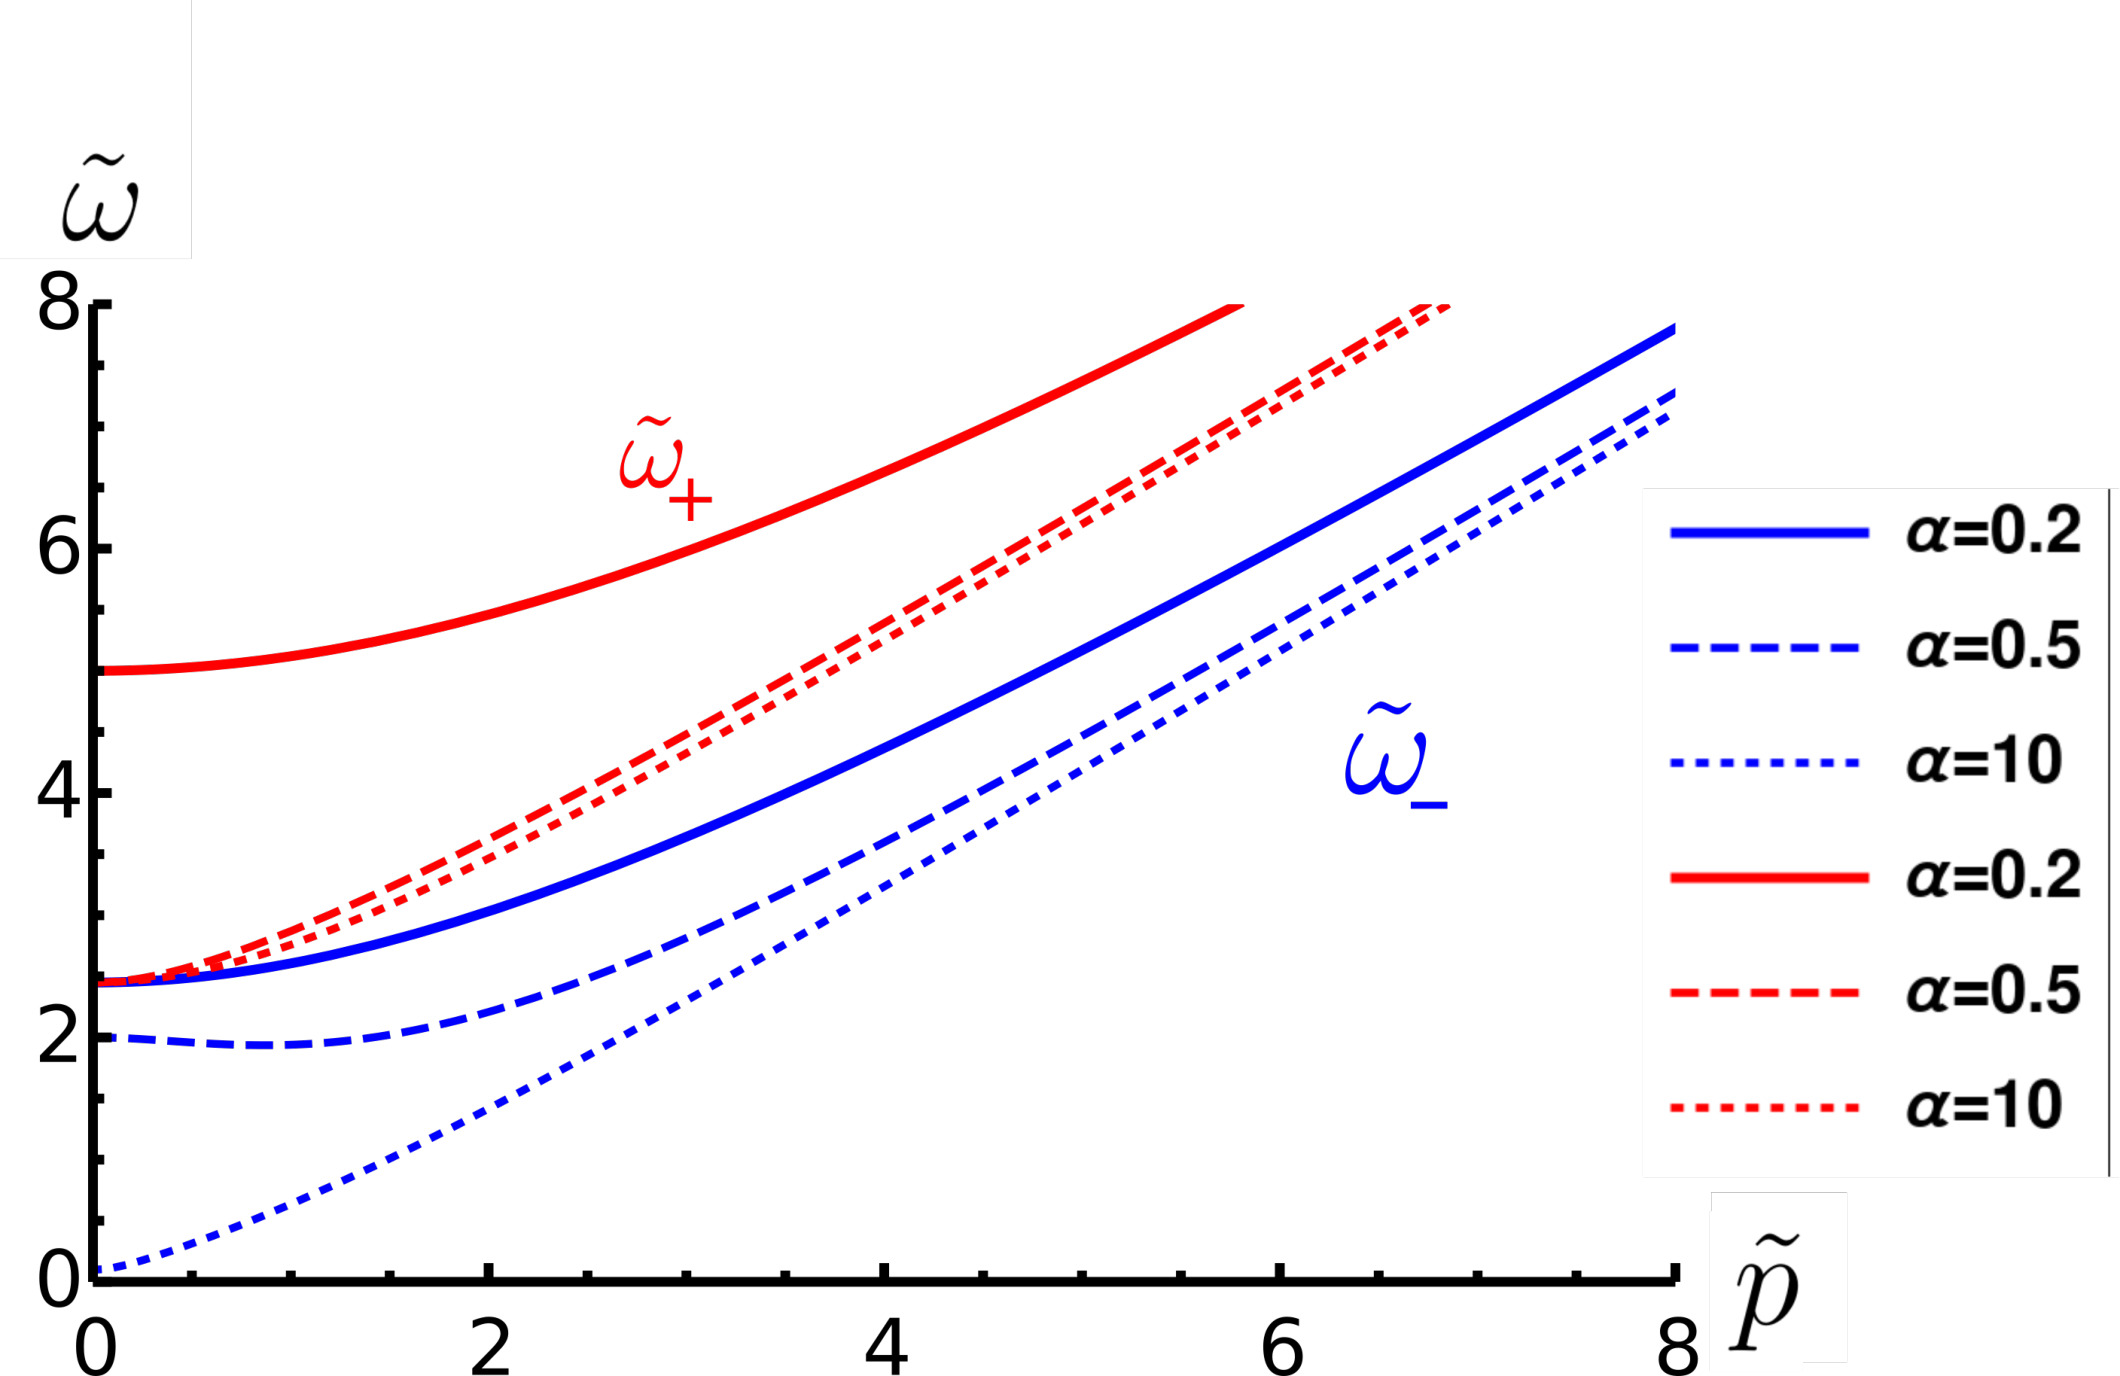
\includegraphics[width=0.55\textwidth]{Chapter_2_Folder_1912.11321/figures/Dispersion_relations-2.pdf}    
    \caption[\textcolor{red}{Dispersion relations for the Abelian Chern-Simons theory in the symmetry broken phase.}]{{\small The dispersion relations of the two branches of perturbative fluctuations for the quartic potential ($s=2$), with different values of the dimensionless coupling $\alpha$.}} \label{fig:dispersion}
    \end{center}
\end{figure}
Depending on the value of $\alpha$, the sign of  $\tilde\omega''_{\pm}(0)$ can be negative which implies a minimum in the dispersion relation away from $\tilde{\bf p}=0$, also called a magneto-roton minimum. One  of the two branches  will exhibit a magneto-roton minimum  for values of $\alpha$ in the range:
\be
\quad\frac{1}{\sqrt{2(s+3)}} < \alpha <  \frac{1}{\sqrt{2(s-1)}}\,.
\ee

\section{Vortex equations}
We want to solve the equations of motion in polar coordinates. Therefore, allowing for a non-trivial spatial metric $h$, the static field equations are:
 \bea
        &&\tfrac{1}{\sqrt h}\partial_j \left(\sqrt h\,\partial^j\Phi\right) - \tfrac{i}{\sqrt{h}} \partial_{j} \left(\sqrt{h} A^{j} \Phi \right) + (\mu +A_0)^2 \Phi -i A_{j} \partial^{j} \Phi - A_{j} A^{j} \Phi\, =\, 
%        \\\nonumber&&\hspace{4in}
  g_{2s} |\Phi|^{2s-2}\Phi \nonumber\\\\\nonumber
        &&\frac{k}{2 \pi} \epsilon^{\sigma \nu \rho} \partial_{\nu} A_{\rho}\, = \,-\sqrt{h}\left[i \left(\partial^{\sigma} \Phi \Phi^{\dag} - \Phi \partial^{\sigma} \Phi^{\dag} \right) \,+\,2 A^{\sigma} \left|\Phi \right|^2- \delta_{0 \sigma} \left(2 \mu \left|\Phi \right|^2 + J_0 \right)\right]\,.
\eea
 As usual, a static vortex configuration carrying $n$ units of magnetic flux is described by the  rotationally symmetric ansatz in polar coordinates: 
\be
            A_0\, =\, A_0(r) \, , \qquad A_r \,=\, 0, \qquad A_{\theta}\, =\, A_\theta(r), 
\qquad \Phi \,= \,f(r)e^{i n \theta}\,.
        \ee
This ansatz leads to the following system of equations\footnote{We omit the equation of motion for $A_r$ which is automatically satisfied.}:
    \bea
&&        f''+\frac{f'}{r} -\frac{1}{r^2}\left(A_\theta - n\right)^2 f + (A_0+\mu)^2 f\, - g_{2s} f^{2s-1} = 0 \label{eq:radial_scalar}  \\\nonumber\\
 &&       -\frac{f^2}{r}\left(A_\theta - n\right)+ \frac{k}{4 \pi} A_0' =0 \label{eq:radial_Atheta}  \\\nonumber\\
 &&       -f^2 A_0 -\mu f^2 + \frac{k}{4 \pi} \left(\frac{A'_\theta}{r}\right)\,=\, \frac{J_0}{2}\,,\qquad \qquad J_0\,=\,-\,2\mu\,v^2\,. \label{eq:radial_A0}
    \eea
We are looking for a configuration which asymptotes at infinity to the ground state with the fixed non-vanishing background value for $J_0$, obeying the boundary conditions:
        % Boundary Conditions:
        \bea
            A_\theta(r) \xrightarrow{r \to \infty} n\,, \qquad A_0(r) \xrightarrow{r \to \infty} 0, \qquad f(r) \xrightarrow{r \to \infty} v\,, \qquad f(0) = 0\,.
        \eea
With the rotationally symmetric ansatz above, the magnetic field $B$ only depends on $r$, and the configuration carries $n$ units of flux:
\be
B(r)\,=\,\frac{A_\theta'(r)}{r}\,,\qquad\qquad
\Phi_B 
\,=\,\lim_{r\to\infty} \int_0^{2 \pi} A_{\theta}(r)\, d\theta \,=\, 2\pi n\,,
\ee
assuming  $A_\theta$ vanishes at the origin.
\subsection{Qualitative features}
The equation of motion \eqref{eq:radial_A0} for $A_0$, which implements the Gauss constraint, fixes the value of the magnetic field at the core of the vortex where the scalar field vanishes. Thus,
\be
B(0)\,=\,\frac{4\pi}{k}\,J_0
%\,=\,-\frac{4\pi\mu v^2}{k}
\,=\,-\frac{\mu^2}{\alpha}\,,
\ee
where $\alpha$ is the effective coupling defined in \eqref{alpha}. For a given winding number $n$, the value of $\alpha$ completely characterizes the vortex solution when expressed in terms of rescaled dimensionless variables.
The effect of the Gauss constraint is to induce a magnetic field $B$ inside the vortex core to precisely cancel the background source $J_0$ which could also  be viewed as a uniform background magnetic field.  Outside the vortex $B$ vanishes,
\be
\lim_{r\to\infty} B(r)\,=\,0\,.
\ee

The sign of $B(0)$ plays an important role in determining the properties of the vortex solutions. Without loss of generality, we assume that the chemical potential $\mu$ and the Chern-Simons level $k$ are both positive:
\be
\mu >0\, \qquad \qquad k >0\,.
\ee
With this choice $B(0)$ is negative definite,   independently of the sign of the magnetic flux $2\pi n$. However, this means that solutions with positive and negative flux will be qualitatively different. This breaking of charge conjugation is precisely what we expect in the presence of the $U(1)$ chemical potential.

\paragraph{Negative flux $n<0$}: Assuming that the magnitude of the magnetic field $|B(r)|$ increases monotonically towards the vortex core, and given that the value of the core magnetic field is independent of $|n|$ (the number of units of flux) the vortex core size should  increase with $|n|$ for negative $n$. Taking $B$ to be uniform within the core for large enough $|n|$, we can estimate the radius $R_n$ of a vortex solution with $|n|\gg 1$:
\be
|B(0)|\pi R_n^2 \,\approx \, 2\pi |n| \,\quad\implies\quad R_n\,\approx\,\frac{\sqrt{2\alpha|n|}}{\mu}\,,\quad |n|\gg1\,.
\label{radius}
\ee
The assumption of uniformity of the vortex core region is self-consistently justified by first noting that for small $r$,
\be
f(r)\,=\,c_0\,r^{|n|} +\ldots\,,\qquad \qquad c_0 >0\,.
\ee 
This is obtained by neglecting $A_\theta$ in comparison to $n$, and ignoring higher order terms for small $r$ in eq.\eqref{eq:radial_scalar}. 
Therefore, for large flux, the scalar profile is extremely flat near $r=0$. With a uniform $B$ field in the vortex interior, the vector potential is determined as 
\be
 A_\theta\approx-\frac{1}{2} |B(0)| r^2\,,
\ee
and this approximation breaks down precisely when $r\approx R_n$
(see eq.\eqref{radius}) . 
We see numerically that the scalar field profile,  inside the vortex, closely follows the solution to the first order equation:
\bea
&&f'(r)\,\approx\,\tfrac{1}{r}\left(|n|-\tfrac{1}{2}|B(0)|r^2\right)\, f(r)\\\nonumber\\\nonumber
\implies \quad&&f(r)\approx c_0 r^{|n|}\,e^{-|B(0)|r^2/4}\,,\quad r< R_n\,.
\eea
This feature of the solution  is depicted in figure \ref{fig:firstorder}. 

The equation of motion \eqref{eq:radial_Atheta} for $A_\theta$ determines the  radial electric field $E(r)\,=\,A_0'(r)$. 
The electrostatic potential $A_0$ remains constant inside the core region since $f(r)$ is vanishingly small and therefore the electric field is also vanishingly small. 
Outside the core region the electric and magnetic fields decay exponentially to zero. Linearizing about the asymptotic solution at  large $r$ we find,
\bea
&&\delta f\,\equiv\, f(r)-v\,,\qquad \delta A_\theta\,=\, A_\theta-n\,,\\\nonumber\\\nonumber
&&\delta A_\theta\,=\,\frac{\alpha}{\mu}\, r A_0'\,,\\\nonumber\\\nonumber
&&\delta f'' \,+\,\frac{\delta f'}{r}\,-\,(2s-2)\mu^2\delta f\,=\, -2 A_0 \mu v\,,\\\nonumber\\\nonumber
&&A_0''\,+\,\frac{A_0'}{r}\,-\,\frac{\mu^2}{\alpha^2}A_0\,=\,\frac{2\mu^3}{v\alpha^2}\delta f\,.
\eea
The solutions to the homogeneous equations for the fluctuations $\delta f$ and $A_0$ are the Bessel functions $K_0\left(\sqrt{2s-2}\mu r\right)$ and $K_0\left(\mu r/\alpha\right)$ respectively, and these control the exponential decay of fluctuations at large $r$,
\be
K_0\left(\sqrt{2s-2}\,\mu r\right)\big|_{\mu r\to\infty} \,\sim\,\frac{e^{-\sqrt{2s-2}\,\mu r}}{\sqrt {\mu r}}\,,\qquad K_0\left(\mu r/\alpha\right)\big|_{\mu r\to\infty} \,\sim\,\frac{e^{-\mu r/\alpha}}{\sqrt {\mu r}} \,.         
\ee
The two exponents are related to  masses of the gapped perturbative excitations around the Higgsed ground state.
Since $A_\theta(r)\simeq n$ outside the core region, according to  eq. \eqref{eq:radial_Atheta} the electric field is only significant in a strip  along the edge of the vortex core.  Numerically, we find that the width of this strip does not scale with $|n|$, so that in the limit of large $|n|$, the contribution from the transition region to the vortex energy is subleading in $|n|$. 

We will see below that these qualitative aspects of the vortex solutions lead to linear dependence of the vortex energy on $|n|$ and BPS-like behaviour at a critical value of the effective coupling $\alpha$.

\textbf{Positive flux $n>0$:} Positive flux solutions are qualitatively distinct from the negative flux ones.  This is because $B(0)<0$ independent of $n$, so 
$B(r)$ must switch sign to yield a net positive flux.  For large $n>0$, most of this positive flux remains concentrated in a ring-like region at the edge of the vortex. In this case the total flux can be written as a sum of two contributions, one that scales with the area of the vortex and is negative, therefore must be subleading, and a positive dominant contribution which scales with the radius of the configuration\,,
\be
2\pi n\,\sim\, -\pi R_n^2\frac{\mu^2}{\alpha}\,+\, 2\pi R_n \Delta_{\rm ring} \, B_{\rm ring}\,.\label{ringansatz}
\ee
Here $\Delta_{\rm ring}$ is the width of the  edge region which we take to be independent of $n$, whilst 
$B_{\rm ring}$
% \sim n^\beta$ 
denotes the peak value of the magnetic field in the ring and $R_n$ 
%\sim n^\gamma$ 
is the radius of the vortex for large enough $n$. The negative area-dependent contribution  is a key difference from a similar situation discussed in \cite{Bolognesi:2007ez}.  We cannot exclude the possibility that both the area and perimeter 
contributions have faster than linear growth and a delicate cancellation yields the correct flux. It is possible to suppress the area contribution by making $\alpha$ arbitrarily large. The large $\alpha$ limit makes the magnetic field inside the vortex vanishingly small and the system then closely resembles an abelian  Chern-Simons vortex in vacuum.  
%If the area dependent term is to be subleading then the exponent $\gamma < \frac{1}{2}$, while $\gamma+\beta+\varepsilon=1$. 
\section{Vortex energy and BPS-like scaling}
The ``energy" functional appropriate for the grand canonical ensemble is the grand potential. The Chern-Simons term does not contribute to it for static configurations. The grand potential is obtained by using the Lagrangian density \eqref{lagfull} with $\mu\neq 0$ and passing to the Hamiltonian picture. Rewriting the Hamiltonian in terms of the fields and their derivatives, the desired energy functional is\footnote{For static configurations, the grand potential can be quickly derived by retaining only the spatial gradient and potential terms including the Chern-Simons density,
 \bea
\mathcal{E} \,=\,\int d^2 x 
 \left( \left| D_i \Phi\right|^2 \,- \,\left(A_0+\mu\right)^2 \left| \Phi\right|^2  %-2 \mu A_0 \left|\Phi\right|^2 -\mu^2 \left| \Phi\right|^2 
 + A_0\left(\frac{k}{2 \pi}  B -J_0\right)+ \frac{g_{2s}}{s}  \left| \Phi\right|^{2s}\right)\,,
 \eea
 and then applying the constraint \eqref{constraint}.
},
\bea
{\cal E}\,=\,\int d^2 x 
 \left( \left| D_i \Phi\right|^2 \,+ \,A_0^2 \left| \Phi\right|^2  %-2 \mu A_0 \left|\Phi\right|^2 -\mu^2 \left| \Phi\right|^2 
 %+ A_0\left(\frac{k}{2 \pi}  B -J_0\right)
 +\frac{g_{2s}}{s}  \left| \Phi\right|^{2s}-\mu^2\left| \Phi\right|^2\right)\,,
 \eea 
 accompanied by the constraint which incorporates the effect of the Chern-Simons term,
 \be
\frac{k}{4\pi} B\,=\,A_0|\Phi|^2+\mu\left(|\Phi|^2-v^2\right)\,.\label{constraint}
 \ee
 
An interesting feature of the finite-$\mu$ vortices (with negative flux)  is that they appear to be  marginally bound (or BPS-like) for a specific value of the effective dimensionless parameter $\alpha$. Recall that this parameter depends on the Chern-Simons level, the chemical potential and the interaction strength:
\be
\alpha \,=\,\frac{k\mu}{4\pi v^2}\,=\,\frac{k}{4\pi}\left(\frac{g_{2s}}{\mu^{3-s}}\right)^{\frac1{s-1}}\,.\label{alphadef}
\ee
Let us perform a rescaling of variables and fields so that the equations of motion can be written explicitly in terms of dimensionless quantities:
\be
\tilde r\,\equiv\,\mu r\,,\qquad \tilde f\,\equiv\, \frac{f}{v}\,,\qquad a\,\equiv\,\frac{1}{\tilde r} \left(A_\theta-n\right)\,,\qquad \tilde A_0\,\equiv\,\frac{A_0}{\mu}\,.
\ee
The rescaled scalar profile vanishes at  $\tilde r=0$ and approaches unity for large $\tilde r$: $\tilde f(\tilde r\to\infty)=1$.  The asymptotic behaviours of $a(\tilde r)$ and $\tilde A_0$ are,
\be
\lim_{\tilde r\to 0}\tilde r a(\tilde r)\,=\,-n\,,\qquad \lim_{\tilde r\to \infty}\tilde r a(\tilde r)\,=\,0\,,\qquad \lim_{\tilde r\to \infty}\tilde A_0(\tilde r)=0\,.
\ee
The resulting dimensionless equations of motion (primes denote derivatives with respect to $\tilde r$) are,
 \bea
 &&\tilde f'' + \frac{\tilde f'}{\tilde r} - a^2\, \tilde{f} + \left(\tilde A_0+1\right)^2\tilde{f}  -\tilde f^{2s-1} =0 \label{eq:dimlesseom1}\\\nonumber\\
&& \alpha \tilde A_0' \,=\,  a\,\tilde f^2 \label{eq:dimlesseom2}\\\nonumber\\
  &&      \alpha \tilde B= \left(\tilde f^2-1\right)+\tilde f^2 \tilde A_0\,.\label{eq:dimlesseom3}
 \eea
Therefore, for a fixed flux $n$, the solutions are only parametrised by the  dimensionless 
effective coupling $\alpha$. Note we have introduced the
dimensionless magnetic field,
\be
\tilde B\,=\,\frac{1}{\tilde r}\,\left(\tilde r a\right)^\prime\,=\,\frac{A_\theta^\prime}{\tilde r}\,.
\ee
We first rewrite the energy functional using the rescaled fields and variables,
\be
{\cal E}\,=\,2\pi v^2\int_0^\infty \tilde r\, d\tilde r\left[\left(\tilde f'- a \tilde f\right)^2 + a\frac{d }{d\tilde r}\left(\tilde f^2-1\right)+\tilde A_0^2\tilde f^2 +\frac{\tilde f^{2s}}{s}-\tilde f^2 +\frac{s-1}{s}
%\frac{1}{\alpha}\tilde A_0\tilde f^2(1-\tilde f^2)
\right]\,,\label{bpsfirst}
\ee
where we have included a constant zero-point shift so that the energy density is vanishing for the ground state at infinity. The second term in eq.\eqref{bpsfirst} when integrated by parts yields a nonvanishing surface contribution,
\be
\int_0^\infty d\tilde r \,\left(\tilde r a\right)\frac{d }{d\tilde r}\left(\tilde f^2-1\right)\,=\,|n|\,-\,\int_0^\infty \tilde r\, d\tilde r \tilde B(\tilde f^2-1)\,.
\ee
Employing the Gauss constraint to eliminate $\tilde B$ in favour of $\tilde A_0$, we obtain an expression for the energy functional which is suitable for subsequent approximations and matching with numerical results,
\bea
{\cal E} = 2\pi v^2 |n| +2\pi v^2\int_0^\infty \tilde r d\tilde r&&\left[\left(\tilde f'-a\tilde f\right)^2+\left(\frac{\tilde f^{2s}}{s}-\tilde f^2 +\frac{s-1}{s}\right)-\frac{1}{\alpha}\left(1-\tilde f^2\right)^2 +\right.\nonumber\\\label{energys}\\\nonumber
&&\left.\tilde A_0^2\,\tilde f^2+\frac{1}{\alpha}\tilde A_0 \tilde f^2(1-\tilde f^2)\right]\,. 
\eea
 \subsection{The quartic potential $s=2$}
Anticipating numerical results in the next section, we can make certain  observations on the energetics of vortex solutions for large negative flux. 

Our arguments rely on the fact that for $n$ sufficiently large and negative, all fields are uniform inside and outside the vortex whose radius scales as $\sqrt{|n|}$ , with a thin transition region whose width does not scale with $n$. In the case of the quartic potential the energy functional is, 
\bea
{\cal E}(n, \alpha)\big|_{s=2} = 2\pi v^2 |n| +2\pi v^2\int_0^\infty \tilde r d\tilde r&&\left[\left(\tilde f'-a\tilde f\right)^2+\left(\tfrac{1}
{2}-\tfrac{1}{\alpha}\right)\left(1-\tilde f^2\right)^2 +\right.\nonumber\\\label{energys2}\\\nonumber
&&\left.+\tilde A_0^2\,\tilde f^2+\tfrac{1}{\alpha}\,\tilde A_0 \tilde f^2(1-\tilde f^2)\right]\,. 
\eea
We know that $\tilde f$ vanishes inside the vortex, whilst $\tilde A_0$  and $a(r)$ vanish outside it.  Specifically when $\alpha=2$, the scalar potential is precisely cancelled, and the integrand in the expression above has support only within the transition region at the edge of the vortex. If we assume that this  contribution does not scale with $n$, we conclude that
\be
{\cal E}(n, \,\alpha=2)\big|_{s=2, |n|\gg1}\,=\, 2\pi v^2 |n|\,.
\ee
Our numerical solutions confirm (figure \ref{fig:massn1}) this conclusion which works remarkably well even for low values of $n$, including  $|n|=1,2 \ldots$. Another surprising feature of the solutions for $\alpha=2$ is that they appear to solve the first order equation $\tilde f'= a \tilde f$ to very high numerical accuracy (figure \ref{fig:firstorder})\footnote{In this context, it is worth noting that if the terms proportional to $\tilde A_0$ are omitted (or assumed to be negligible) in eqs. \eqref{eq:dimlesseom1} and \eqref{eq:dimlesseom3}, then the resulting equations coincide, for a particular value of $\alpha$, with equations of motion for a BPS vortex in $U(2)\times U(2)$ ABJM theory which solves an equivalent first order system \cite{0906.2366}.}.


It is easy to extend the arguments to  other values of $\alpha$. When $\alpha\neq 2$, the second term in the integrand of \eqref{energys2} provides an approximately constant energy density inside the vortex where $\tilde f=0$, while all other contributions remain vanishingly small. We therefore find,
\be
{\cal E}(n, \,\alpha)\big|_{s=2, |n|\gg1}\,=\, 2\pi v^2 \left(|n|\,+\,\tfrac12 \mu^2R_n^2\left(\tfrac12-\tfrac{1}{\alpha}\right) \right)\,=\,\alpha\pi v^2|n|\,.
\ee
This behaviour is also confirmed numerically in figure \ref{fig:massn1}, albeit only for large $|n|$ as expected. Interestingly, although $v$ and $\alpha$ each  depend on the quartic coupling constant $g_4$, the large-$|n|$ vortex mass formula depends only the Chern-Simons level $k$ and the chemical potential,
\be
{\cal E}(n,\,\alpha)\big|_{s=2, |n|\gg1}\,=\,\alpha\pi v^2|n|\,=\, \frac{k\mu}{4}|n|\,.
\ee

\subsection{General power law potential $(s\geq 2)$}
 The energies of solutions for general power law potentials now work along similar lines.  The integrand in the energy density \eqref{energys} is negligible both inside and outside the vortex when $\alpha=\alpha_c$,
 \be
 \alpha_c= \frac{s}{s-1}.
 \ee 
 At this critical  $\alpha$ we expect solutions with large flux to have energies ${\cal E}(n)\simeq 2\pi v^2 |n|$. When $\alpha$ takes generic values away from  $\alpha_c$, adapting the $s=2$ argument to general power law potentials $\sim g_{2s}|\Phi|^{2s}$  we obtain,
 \be
 {\cal E}(n, \,\alpha; s)\big|_{|n|\gg 1}\,=\,2\alpha\pi v^2|n|\frac{s-1}{s}\,=\,\frac{s-1}{2s}k\mu|n|\,.\label{generalenergy}
 \ee
This result is confirmed by our numerical solutions for the sextic potential below. As before the mass formula is independent of the interaction strength of the potential. We point out however that the radius of the vortex solution $R_n=\frac{1}{\mu}\sqrt{2\alpha |n|}$ depends nontrivially on all parameters. From the definition of $\alpha$ \eqref{alphadef}, increasing the interaction strength (for fixed $\mu$ and $k$) has the effect of increasing the vortex size.
\subsection{Positive flux vortices}
With our choice of conventions  $\mu >0$ and $k>0$, positive flux solutions are energetically disfavoured. To see this, let us  reconsider the energy functional \eqref{bpsfirst}.  As in the case of the flux in eq.\eqref{ringansatz}, there are different types of contributions to the energy, those that scale with the area of the vortex, those that scale with the perimeter, and finally (gauge-covariant) gradient  terms which become important at the edge of the vortex.
If we pick $\alpha$ to be sufficiently large so that we can ignore the flux contribution from the vortex interior, then 
$B_{\rm ring}\sim n/R_n$. Then the leading contributions to the energy take the schematic form,
\be
{\cal E}(n)\sim (2\pi v^2)\left(\frac{n^2}{R_n}\Delta + c_0\pi R_n^2 \right)\,,\qquad \alpha\gg1
\ee
Here the first term is a perimeter contribution from a covariant gradient while the second term is a potential energy contribution from the interior. Extremizing with respect to $R_n$, we obtain $R_n\sim n^{2/3}$ and ${\cal E}(n)\sim n^{4/3}$.
However this argument will fail for  finite $\alpha$ since $B(0)=-\mu^2/\alpha$ and the area scaling as $n^{4/3}$ would violate  the flux condition \eqref{ringansatz}.  We have not found a satisfactory scaling argument for finite $\alpha$ and large $n$, but our numerical results indicate a faster than quadratic growth of the energy as a function of $n$ in this situation.


%    \section{Approximately BPS solution}
%
%    Here we will show that this solution is equivalent to the SU(2) supersymmetric BPS solution in the ABJM model in a specific limit. This limit can be derived for a particular value of the dimensionless coupling $\alpha$, when a certain heuristic argument about the integral of $A_0(r) f(r)$ holds. We begin by integrating out the magnetic field through the $A_0$ equation of motion \ref{eq:dimlesseom3}.

\section{Numerical results}
The vortex equations of motion are not analytically solvable. We numerically solve the dimensionless equations of motion \eqref{eq:dimlesseom1}, \eqref{eq:dimlesseom2} and \eqref{eq:dimlesseom3} along with the accompanying boundary conditions. Below we outline the results for the quartic potential $(s=2)$ first, and subsequently  summarize the results for the sextic $(s=3)$ case.
\subsection{Quartic potential $(s=2)$}
\paragraph{Negative flux solutions:} A well known feature of Chern-Simons-Higgs vortices in vacuum is the ring-like profile of electric and magnetic fields \cite{0811.2094}. The finite density vortices we have studied are qualitatively distinct and
retain this feature only partially. Figure  \ref{fig:scalarneg}  shows the (dimensionless) scalar field $\tilde f(\tilde r)$ and magnetic field $\tilde B(\tilde r )$  at $\alpha=5$ and different negative values of the magnetic flux.
\begin{figure}[H]
\begin{center}
    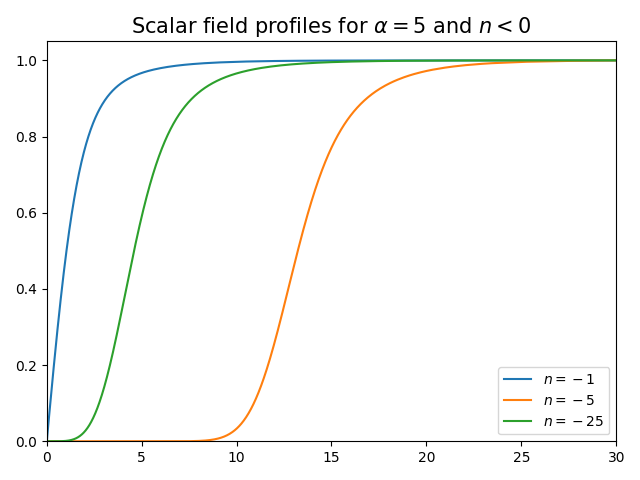
\includegraphics[width=3in]{Chapter_2_Folder_1912.11321/figures/f_alpha_5_final.png}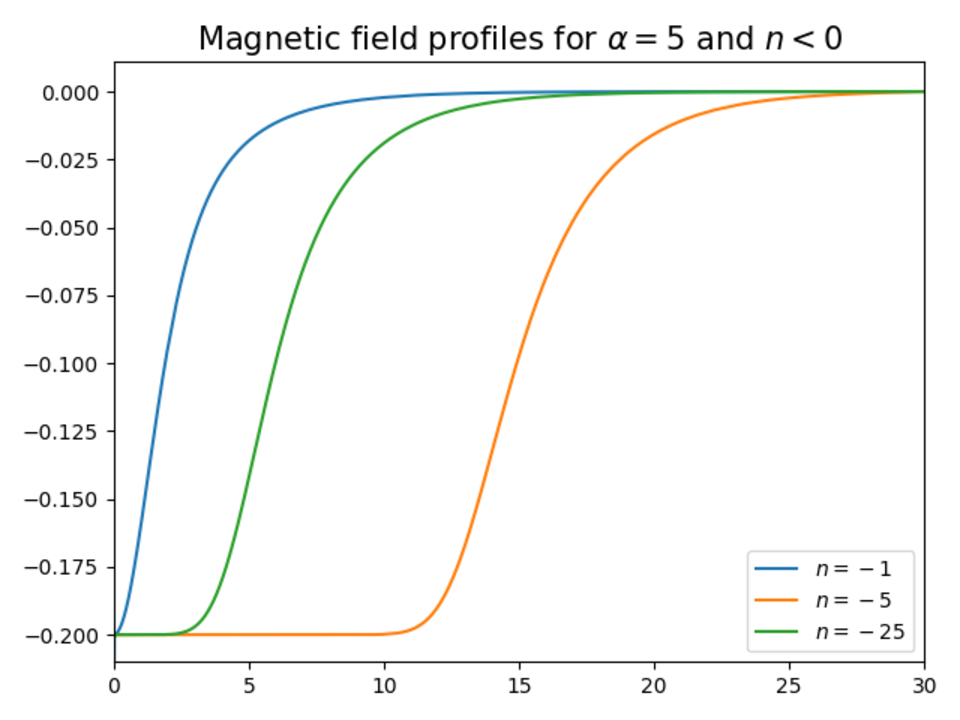
\includegraphics[width=3in]{Chapter_2_Folder_1912.11321/figures/B_alpha_5_final.pdf}
    \caption[\textcolor{red}{This figure showcases the scalar and magnetic field profiles of vortices in the Abelian Chern-Simons model at finite chemical potential and negative magnetic flux.}]{ {\small{\it Left}: The scalar field profile $\tilde f(\tilde r)$ for $\alpha=5$ and negative flux. {\it Right:} The dimensionless magnetic field $\tilde B(\tilde r)$ for the same values of $\alpha$ and magnetic flux.}} \label{fig:scalarneg}
   \end{center}
\end{figure}
Unlike Chern-Simons vortices in vacuum \cite{0811.2094, Bolognesi:2007ez} the magnetic field is no longer expelled from the core of the vortex. Instead, the magnetic field and the scalar are both effectively constant separately inside and outside the vortex and we observe a kink-like transition in between.  The value of the dimensionless magnetic field inside the vortex is $\tilde B(0)= -1/\alpha=-0.2$ for $\alpha=5$. 

\begin{figure}[H]
\begin{center}
    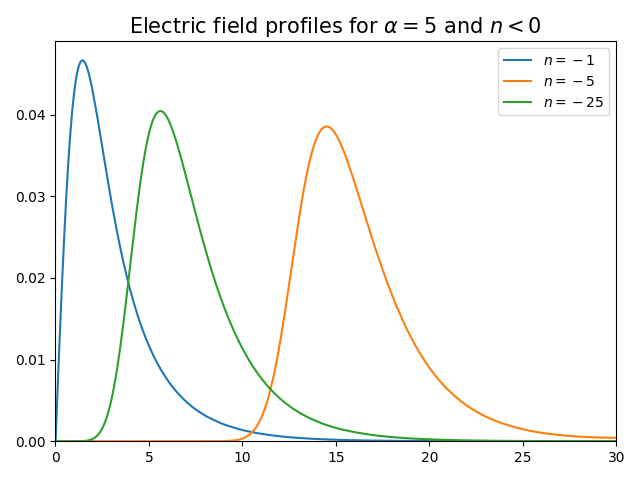
\includegraphics[width=2.8in]{Chapter_2_Folder_1912.11321/figures/E_alpha_5_final.png} 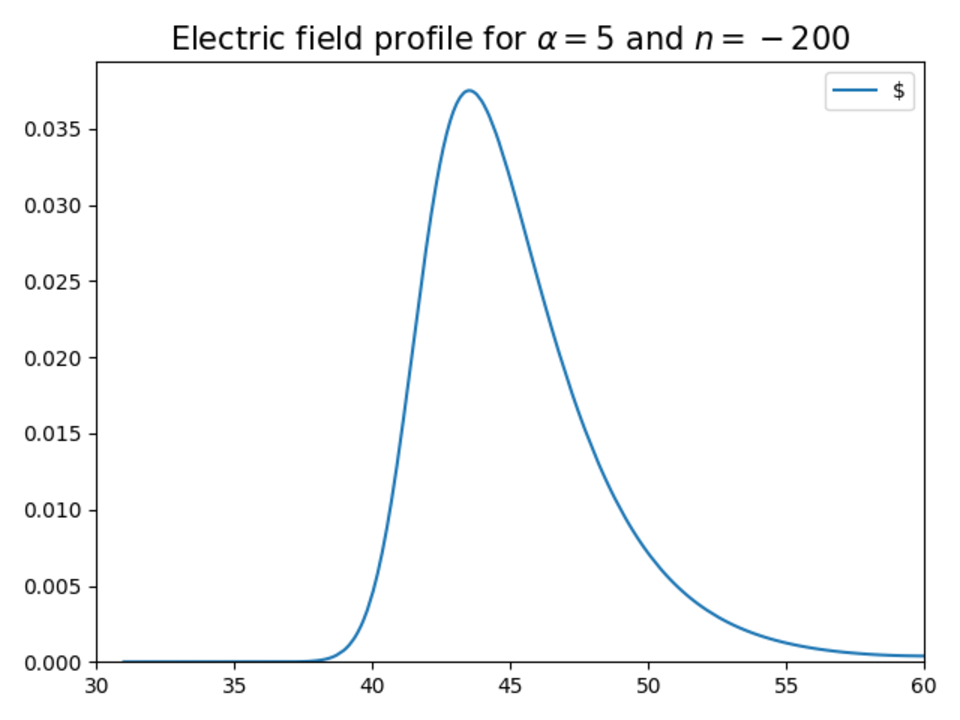
\includegraphics[width=2.8in]{Chapter_2_Folder_1912.11321/figures/E_alpha_5_n_200.pdf} 
    \caption[\textcolor{red}{This figure shows that the electric field profile for the vortex solutions (in the Abelian Chern-Simons model at finite chemical potential and negative magnetic flux) have a ring-like profile.}]{ {\small The electric field has support only at the edge of the vortex implying a ring-like profile. 
   The width of the transition region remains fixed as $|n|$ is cranked up.} }\label{fig:Eneg}
   \end{center}
\end{figure}

 The electric field on the other hand has support only at the edge or the transition-region where the gradient of $A_0$ is significant. This is illustrated in figure \ref{fig:Eneg}.
%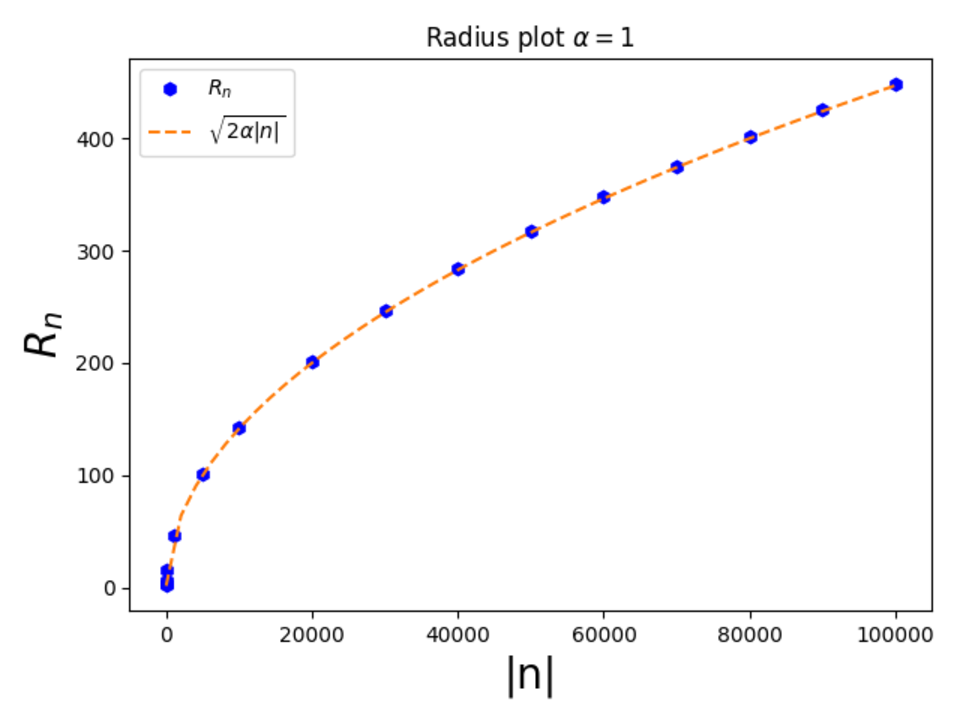
\includegraphics[width=2.9in]{Chapter_2_Folder_1912.11321/figures/radius_alpha1_large_n.pdf}
Even for relatively low values of $|n|$, the location of the peak in the magnitude of the electric field begins to track the large $|n|$ estimate of the vortex radius \eqref{radius}:
\bea
\mu R_n = \sqrt{2|n|\alpha} = \quad
\left\{\begin{matrix}
7.07 & \quad n=-5\,,\alpha=5\\
15.81&\quad n=-25\,,\alpha=5\\
44.7 & \quad n=-200\,,\alpha=5\,.
\end{matrix}\right.
\eea
The width of the ring-like transition region remains fixed as $|n|$ is increased. In particular, both the width of the ring and the peak magnitude of the electric field appear to be solely determined by $\alpha$ for large flux.
\begin{figure}[H]
\begin{center}
    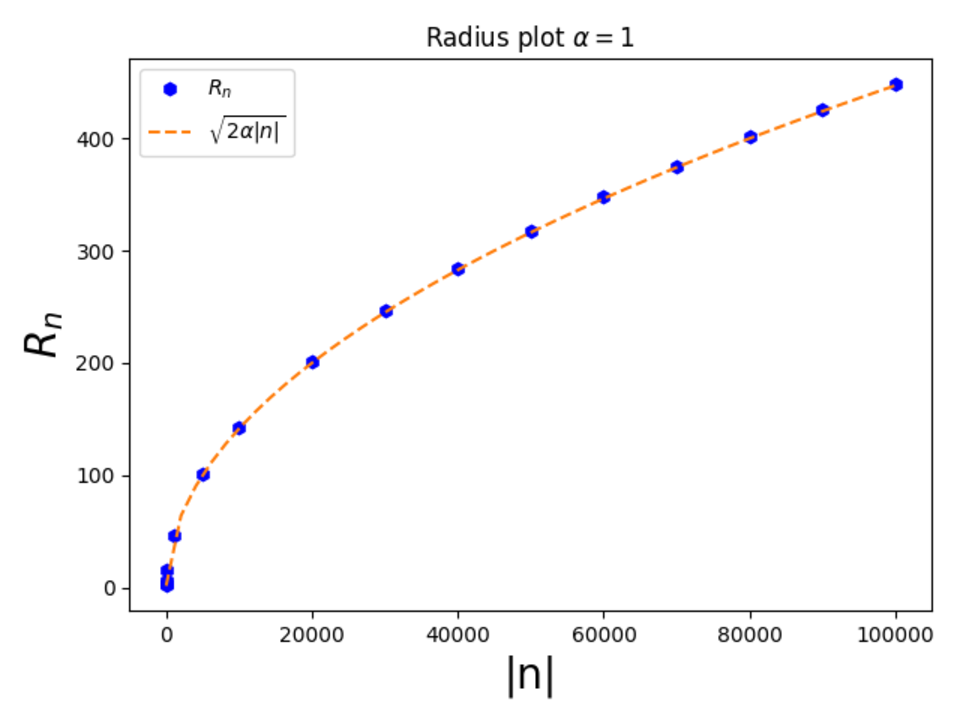
\includegraphics[width=2.9in]{Chapter_2_Folder_1912.11321/figures/radius_alpha1_large_n.pdf}  
    \caption[\textcolor{red}{This figure shows the vortex size dependence on the flux.}]{ {\small The radii of large-$n$ vortex solutions follow very closely the curve $\mu R_n=\sqrt{2\mu |n|}$.
We define the radius of the vortex as the position at which the dimensionless energy density falls below a threshold $\sim 10^{-4}$. } }\label{fig:radius}
   \end{center}
\end{figure}
A precise agreement between the above scaling formula for the radius is obtained when the magnitude of the flux is significantly increased, as shown in the second plot in figure \ref{fig:radius}.

The most interesting aspect of the negative flux vortex solutions is the scaling of the energy with $|n|$. Using the energy functional \eqref{bpsfirst}, we compute the two dimensionless ratios,
\be
\frac{{\cal E}(n, \alpha)}{{|n|\cal E}(1, \alpha)}\,\qquad{\rm and} \qquad \frac{{\cal E}(n, \alpha)}{2\pi v^2|n|} \quad\xrightarrow{|n|\gg 1} \quad\frac{\alpha}{2}\,.\label{ratios}
\ee
The first ratio measures the energy of the $n$-vortex relative to that of $|n|$ vortices each with unit (negative) flux. If this is less than unity, then the $n$-vortex has lower energy than $|n|$ separated $-1$-vortices, and therefore the interactions between them must be attractive (type I). Conversely, if ${\cal E}(n, \alpha) > |n|{\cal E}(1, \alpha)$, the vortex interaction is repulsive (type II). 
\begin{figure}[H]
\begin{center}
 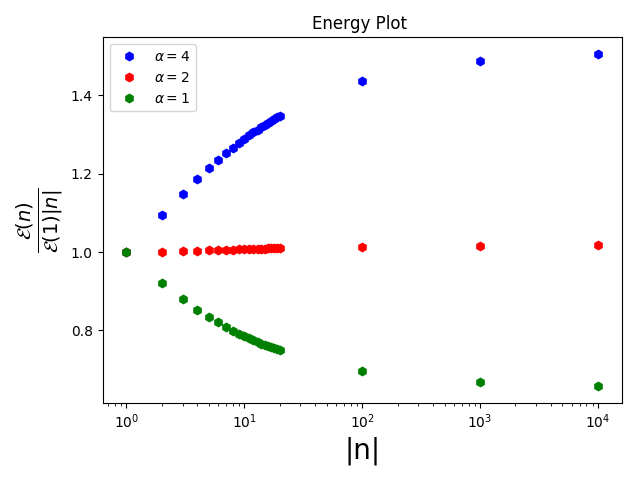
\includegraphics[width=2.70in]{Chapter_2_Folder_1912.11321/figures/bpsrationeg.png}\hspace{0.1in}
    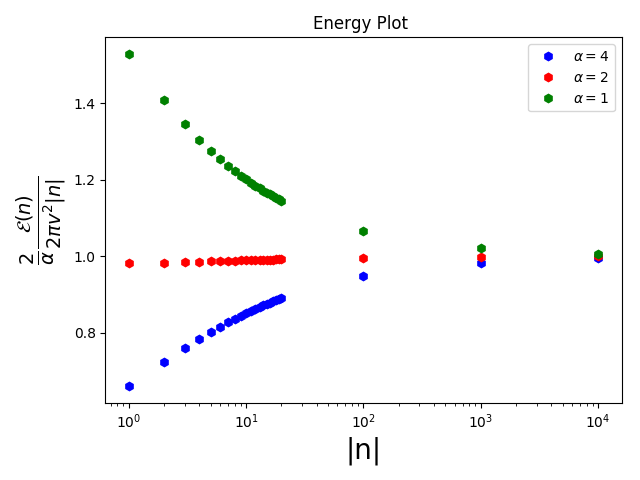
\includegraphics[width=2.70in]{Chapter_2_Folder_1912.11321/figures/mass1neg.png}
    \caption[\textcolor{red}{This figure shows the energy per flux for different values of the coupling parameter $\alpha$.}]{{\small{\it Left:} This shows that $\alpha < 2$ vortices are type I (attractive), separated from type II (repulsive) solutions for $\alpha>2$ by the $\alpha=2$ line where the solutions have vanishing interaction energy. {\it Right:} The $\alpha$-dependence of the $n$-vortex mass formula agrees with analytical arguments at large $|n|$. }} \label{fig:massn1}
   \end{center}
\end{figure}
The second ratio in \eqref{ratios} is the general formula for the $\alpha$-dependence of the $n$-vortex energy which was deduced from arguments for large $|n|$. Figure \ref{fig:massn1} shows to significant numerical precision that negative flux solutions with $\alpha=2$ are effectively ``BPS" for any value of  $|n|$, separating $\alpha> 2$ solutions which are type II (repulsive) from the solutions with $\alpha < 1$ which are type I or attractive. Furthermore the $\alpha$-dependence of the energies of type I and type II vortices for large flux matches the predicted behaviour in eq.\eqref{ratios}. 

A surprising feature of the numerical results is how closely the energies of the vortices with $\alpha=2$  match the BPS result $2\pi |n| v^2$ even for low values of $|n|$. This matching is corroborated by  figure \ref{fig:firstorder}, which shows that the vortex profile for $\alpha=2$  almost solves the first order equation $\tilde f' = a \tilde f$. This figure also demonstrates that the vector potential inside the vortex closely follows the result for a uniform magnetic field.
\begin{figure}[H]
\begin{center}
    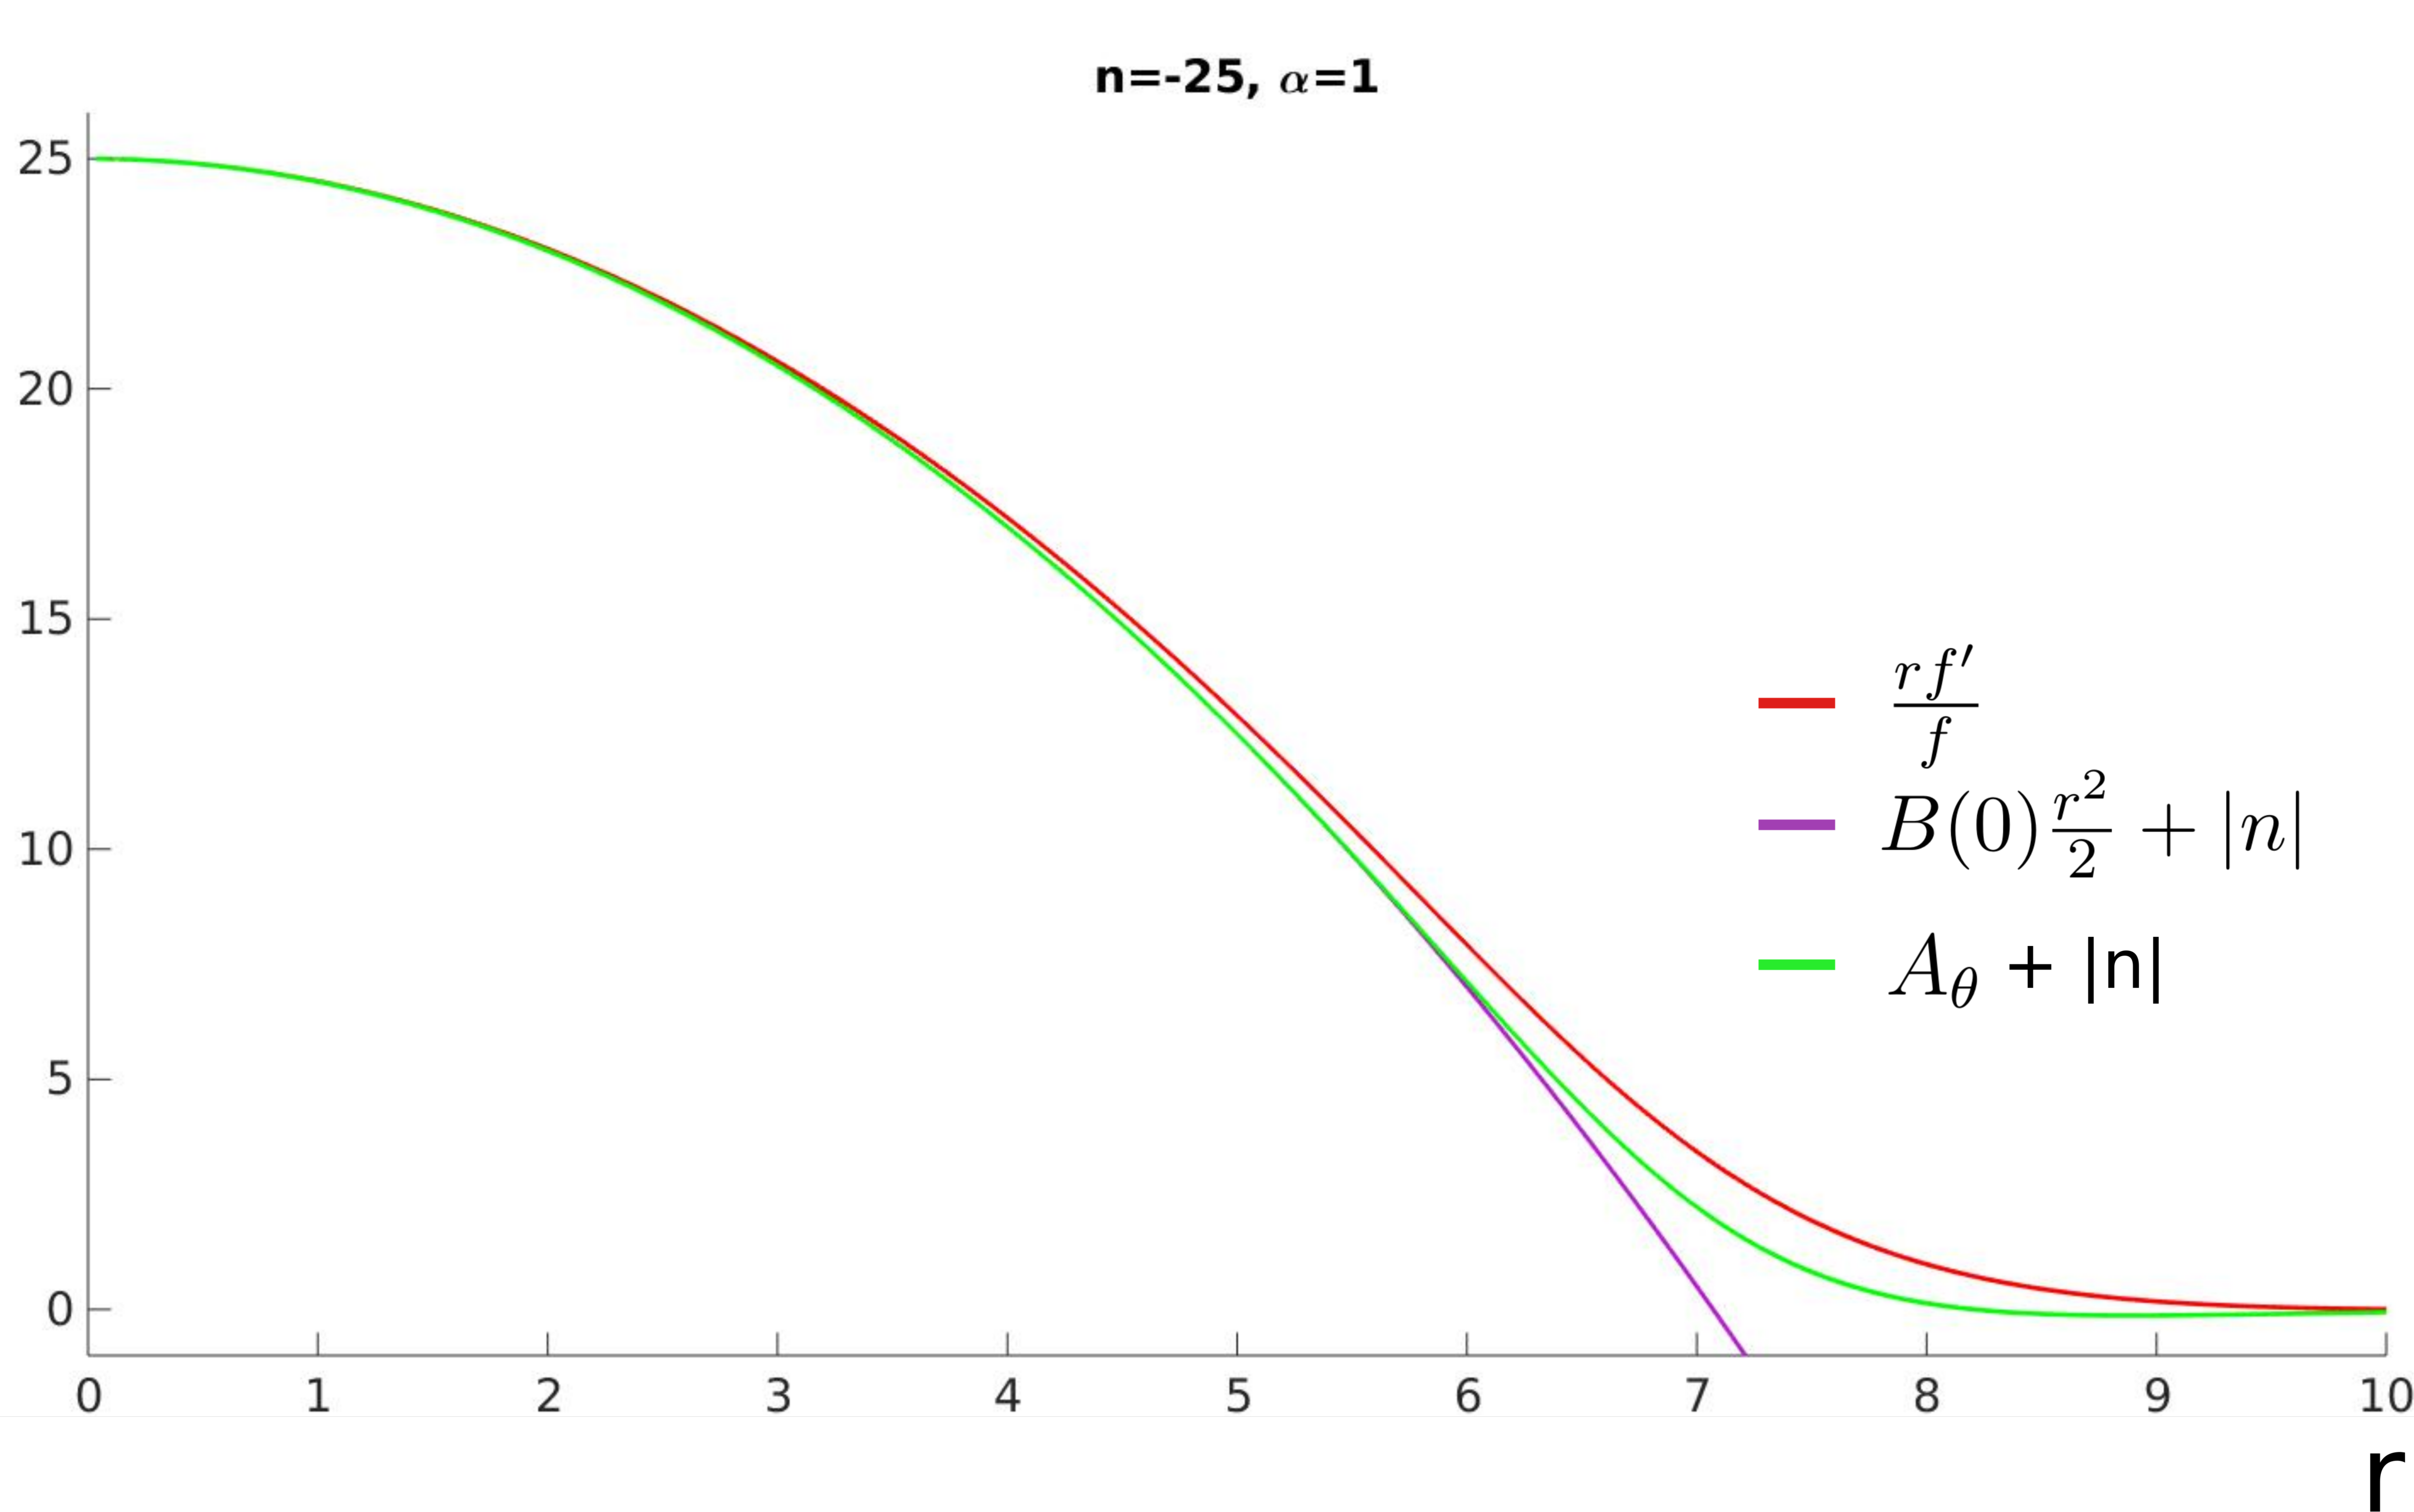
\includegraphics[width=2.70in]{Chapter_2_Folder_1912.11321/figures/firstorderalpha1_corrected.pdf} \hspace{0.1in}
      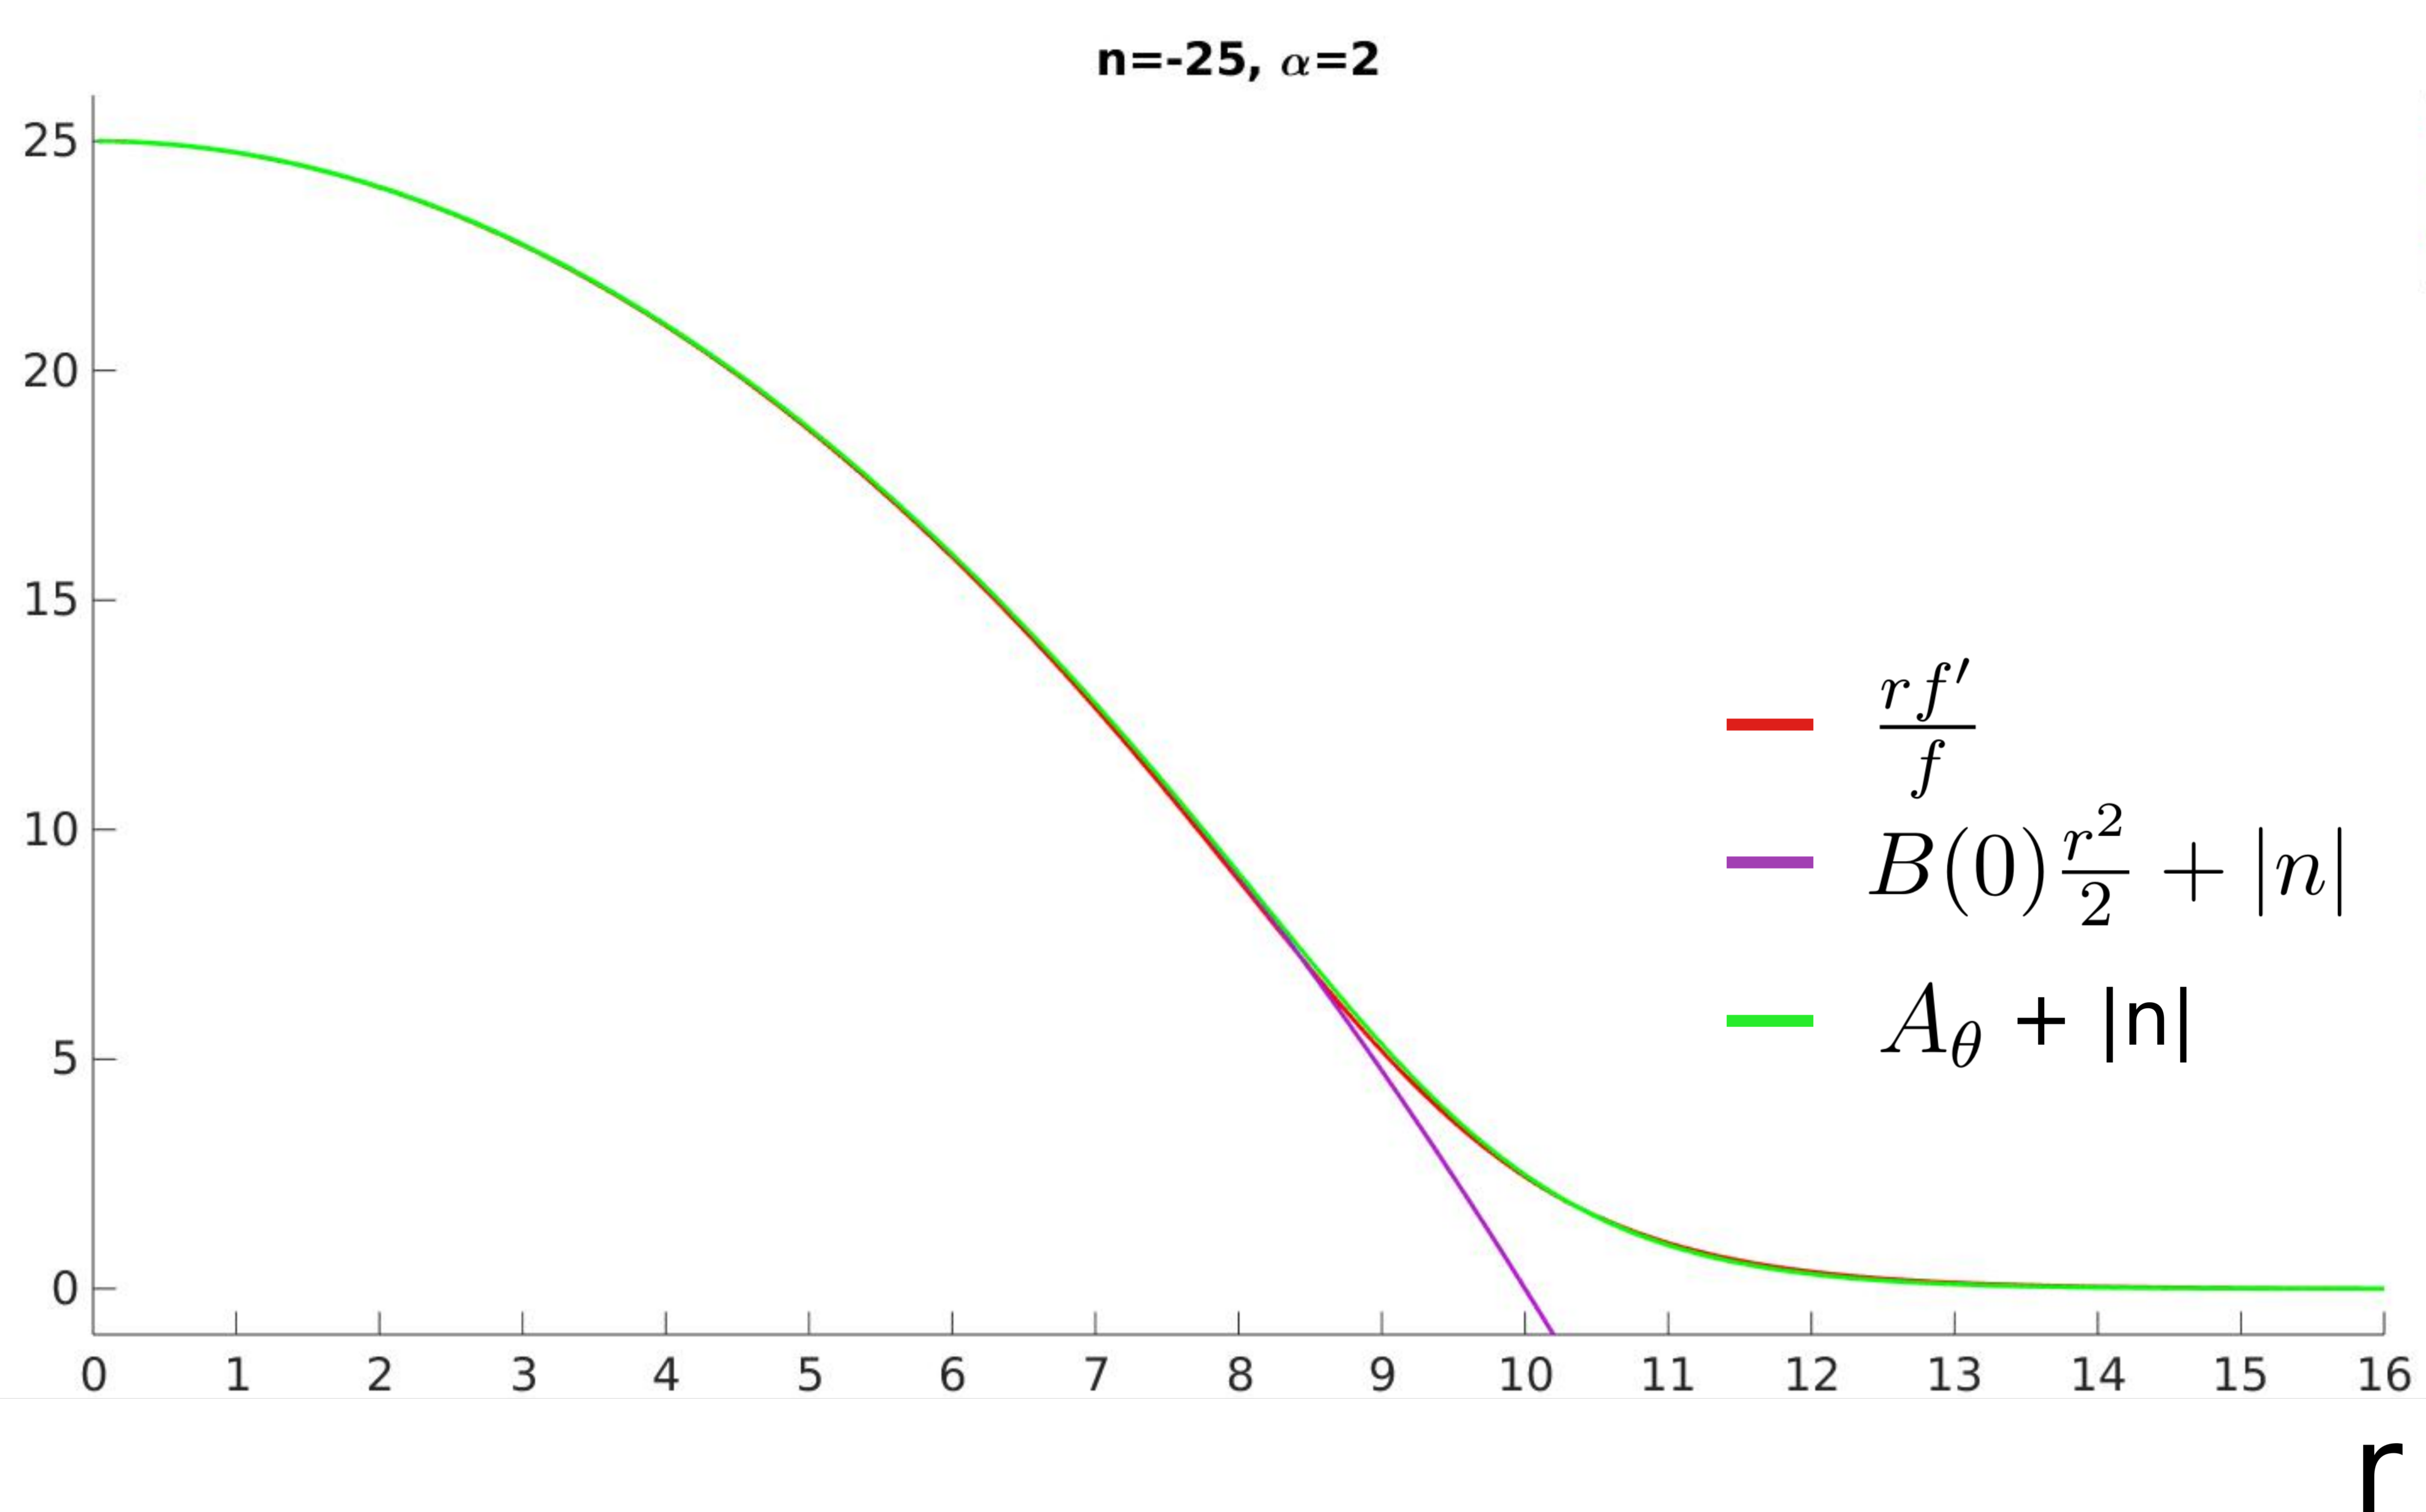
\includegraphics[width=2.7in]{Chapter_2_Folder_1912.11321/figures/firstorderalpha2_corrected.pdf} 
    \caption[\textcolor{red}{This figure shows three quantities that ought to match in the BPS vortex.}]{{\small The figure shows the three quantities: $rf'/f$ (red), $\left(A_\theta+|n|\right)$ (green), and $\left(-|B(0)|r^2/2+|n|\right)$ (purple) evaluated on the exact numerical solutions for $\alpha=1$ and $\alpha=2$.}} \label{fig:firstorder}
    \end{center}
\end{figure}
The extent of the departure of the vortex profile from an exact solution to the  first order equation $\tilde f'=a f$ is shown in figure \ref{fig:error}.  Evaluated on the $\alpha=2$ solution, the quantity $(\tilde f^\prime - a \tilde f)$ deviates minimally from zero near the edge of the vortex.
\begin{figure}[H]
\begin{center}
    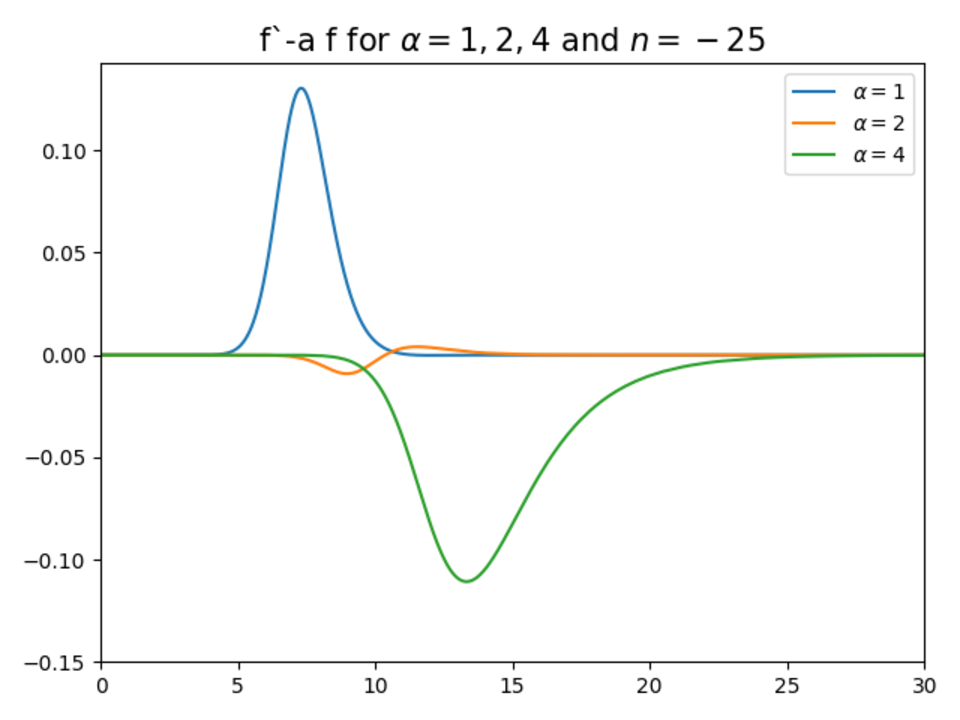
\includegraphics[width=2.6in]{Chapter_2_Folder_1912.11321/figures/BPS_equation_error.pdf}\qquad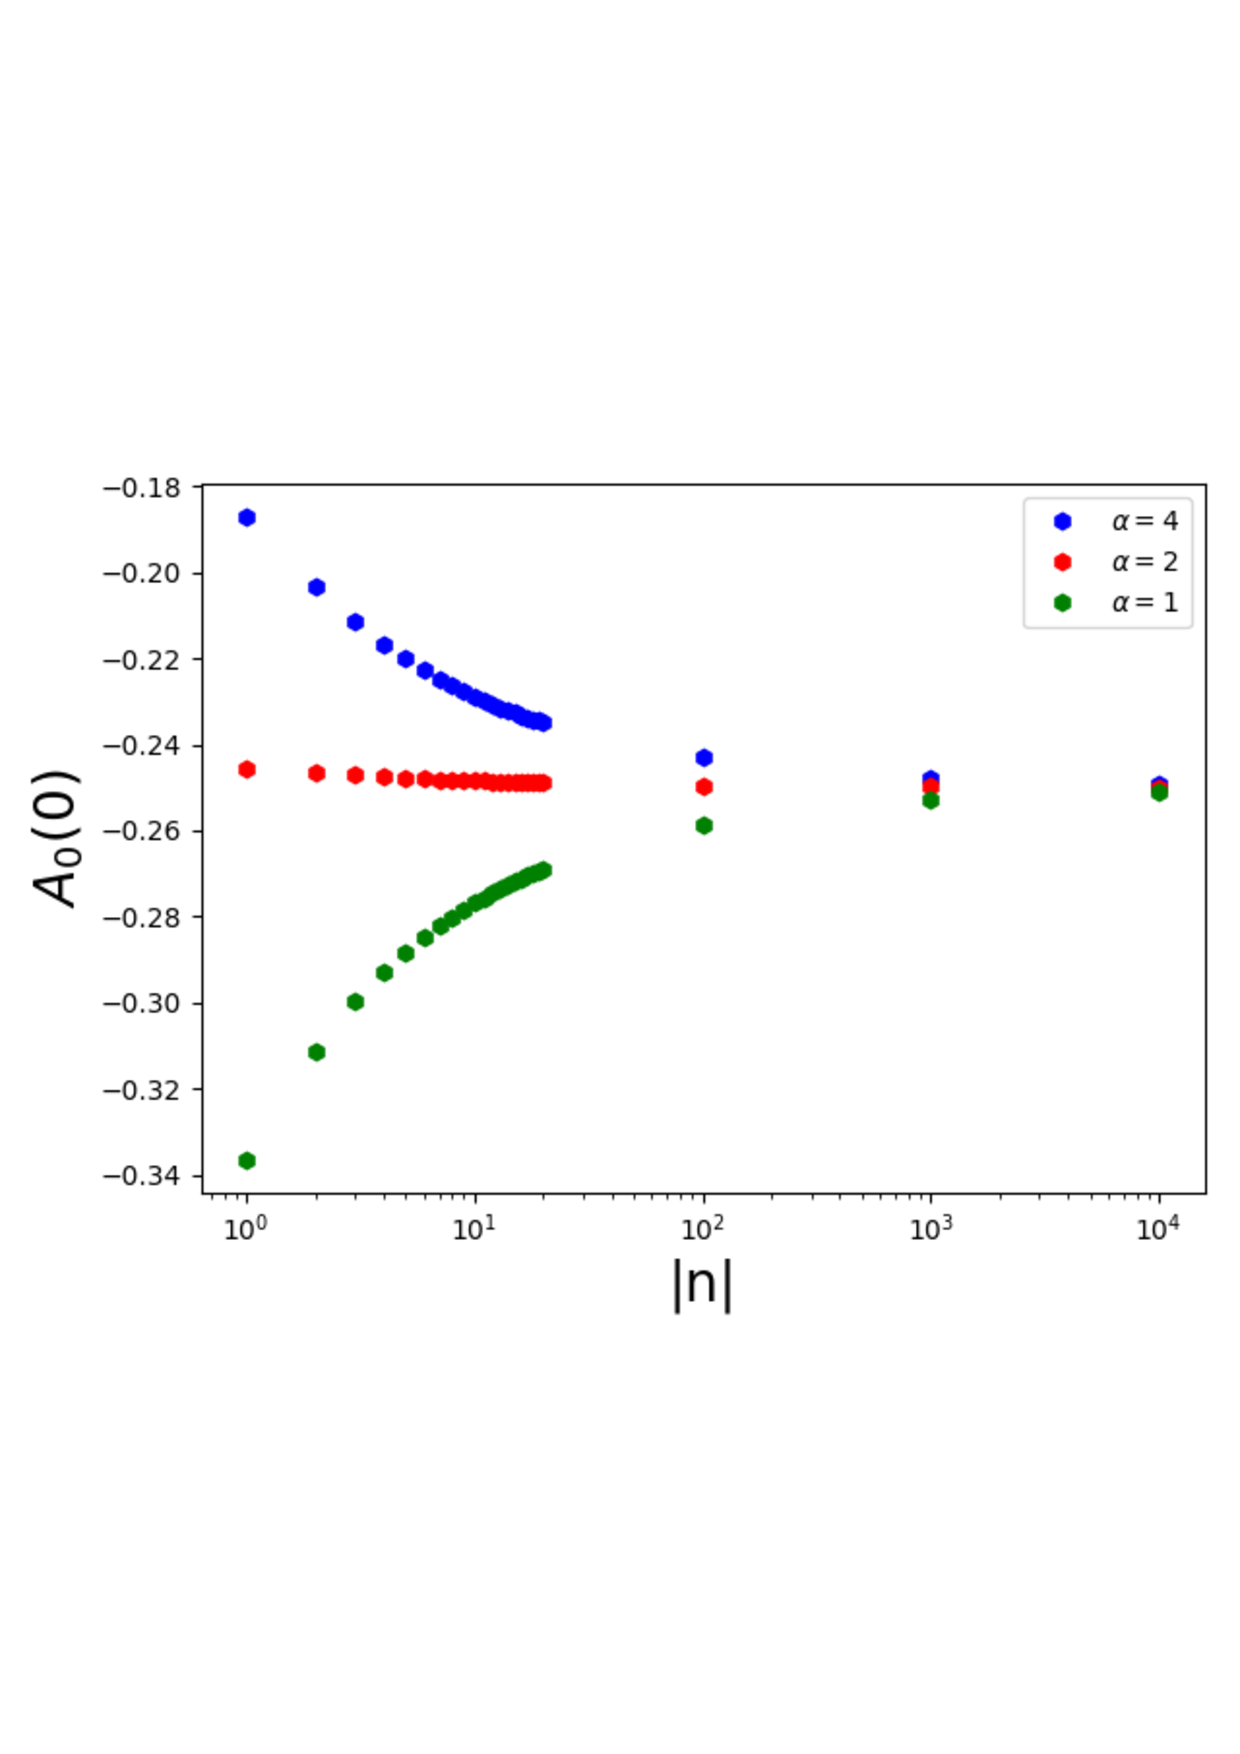
\includegraphics[width=2.6in]{Chapter_2_Folder_1912.11321/figures/negative_n_A0.pdf}
     \caption[\textcolor{red}{Plots of $\tilde{f}(r)' - a(r) \tilde{f}(r)$ for 3 values of $\alpha$ and $\tilde{A}_0(0)$ for different values of $|n|$ and $\alpha$.}]{{\small {\it Left: }$\left(\tilde f^\prime - a \tilde f\right)$ plotted for 3 values of $\alpha$ including critical case. $\alpha=2$. {\it Right:} The value of $\tilde A_0$ at the origin for different $\alpha$ as a function of $|n|$. }} \label{fig:error}
    \end{center}
\end{figure}
Yet another measure of the relevance of the first order equation $\tilde f^\prime = a \tilde f$ for the $\alpha=2$ solutions is given by the value of $\tilde A_0(0)$. The value of the electrostatic potential at the origin is not fixed as a boundary condition, but an output of the solution. Let us use the equation of motion for the electric field \eqref{eq:dimlesseom2} in conjunction with the first order equation at $\alpha=2$,
\be
\tilde A_0^\prime\,=\,\frac{1}{2}a\tilde f^2 \quad\xrightarrow{\tilde f^\prime = a \tilde f}  \quad 
\tilde A_0\,=\,\frac{1}{4}\left(\tilde f^2-1\right)\,,
\ee
where the integration constant on the right hand side is fixed by requiring that $\tilde A_0$ vanishes as $r\to\infty$. 
We therefore arrive at a prediction,
\be
\tilde A_0(0)\big|_{\alpha=2}\,=\,-\frac{1}{4}\,.
\ee
This is precisely what we see in figure \ref{fig:error} for the $\alpha=2$ solution. However, we also find the unexpected feature that $\tilde A_0(0)$ for other values of $\alpha$ approaches $-1/4$ at large $|n|$. This suggests  that solutions with generic $\alpha$ and large $|n|$ are not approximate  solutions to the first order equation\footnote{For generic $\alpha$, eq. \eqref{eq:dimlesseom2} along with the first order equation $\tilde f^\prime = a \tilde f$, would imply $\tilde A_0(0)=-1/2\alpha$. }.
\paragraph{Positive flux solutions:}
We have explained how positive flux vortex solutions are qualitatively distinct from negative $n$ solutions. In certain limits (large-$\alpha$) they closely resemble  Chern-Simons vortex solutions in vacuum. 
The majority of the flux resides in the ring region or edge of the solution as $n$ is increased (see figure \ref{positiveprofile}).
\begin{figure}[H]
\begin{center}
 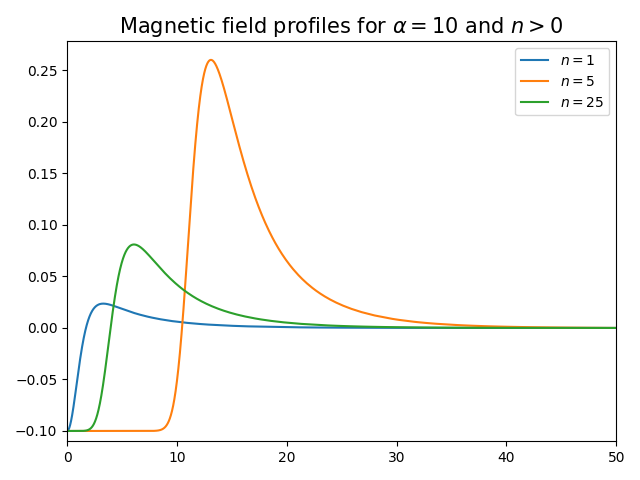
\includegraphics[width=2.7in]{Chapter_2_Folder_1912.11321/figures/B_alpha_10_positive_final.png} 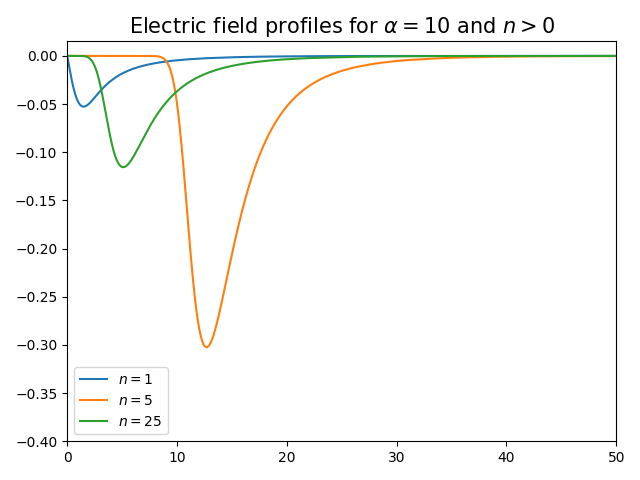
\includegraphics[width=2.7in]{Chapter_2_Folder_1912.11321/figures/E_alpha_10_positive_final.png}
     \caption[\textcolor{red}{This figure depicts the magnetic and electric field profiles for positive flux.}]{{Magnetic and electric fields for positive flux vortices have support near the edge of the vortex and their peak values grow without bound as $n$ is increased.}} \label{positiveprofile}
    \end{center}
\end{figure} 
In figure \ref{positiveenergy} the dependence of the $n$-vortex energy on $|n|$, is displayed for the negative and positive flux solutions, and as expected the latter are more massive.  It is surprising  that ${\cal E }(n)/|n|$ appears to grow faster than $|n|$.
\begin{figure}[H]
\begin{center}
 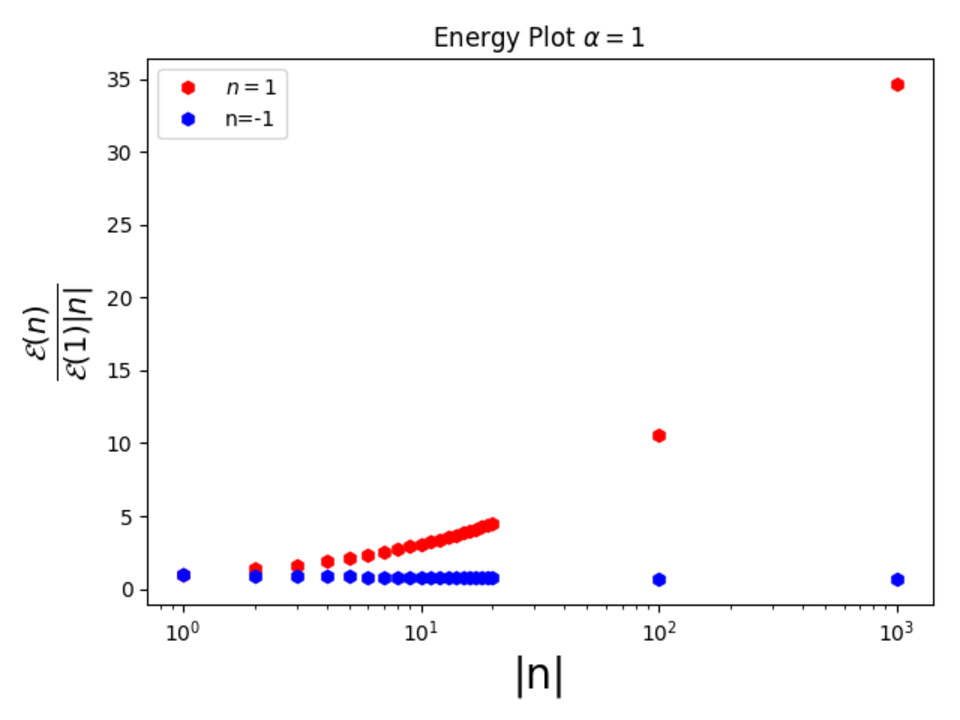
\includegraphics[width=3in]{Chapter_2_Folder_1912.11321/figures/positive_n_energy.pdf}
     \caption[\textcolor{red}{Energy per flux for positive winding number $n$.}]{{\small Positive flux vortices have higher energy than their negative flux counterparts.}} \label{positiveenergy}
    \end{center}
\end{figure}
\subsection{Sextic potential ($s=3$)}
Finally we turn to numerical results for the higher power law potentials, in particular the $s=3$
or sextic potential. We do not expect to see major qualitative differences overall. One special feature of the quartic potential $(s=2)$ is that when $\alpha=2$, there is a precise cancellation of the scalar potential energy contribution to the energy functional. This is not the case for general power laws. Nevertheless there is an approximate cancellation when evaluated on the vortex background at the critical value of $\alpha = \frac{s}{s-1}$.   The critical value for the sextic potential is $\alpha = \frac32$.
The profiles for the negative flux vortex with sextic and quartic potentials are shown on the same plot in figure \ref{sexticprofile}. For the same values of the dimensionless parameter $\alpha$ there is very little difference between the two systems. The transition between the two phases is slightly steeper for the sextic potential. The ratios of the energies of the $n$-vortex to single vortex and and the BPS value ($2\pi v^2 n$) are shown in figure 
\ref{sexticenergy}.

\begin{figure}[H]
\begin{center}
 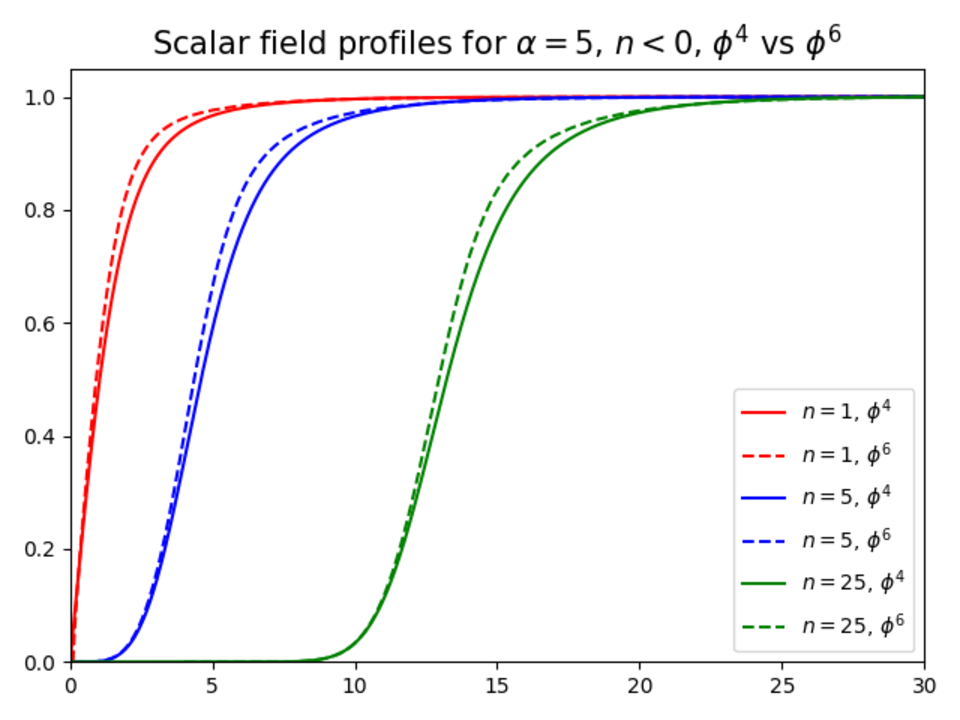
\includegraphics[width=1.85in]{Chapter_2_Folder_1912.11321/figures/f_sixthvsfourth.pdf}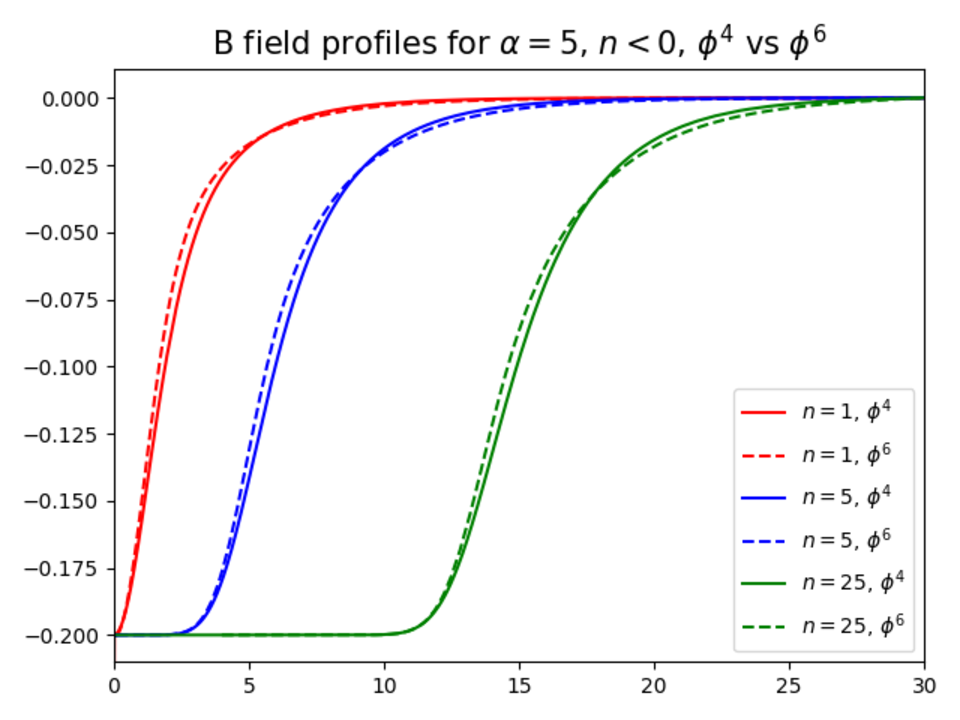
\includegraphics[width=1.85in]{Chapter_2_Folder_1912.11321/figures/B_sixthvsfourth.pdf}
 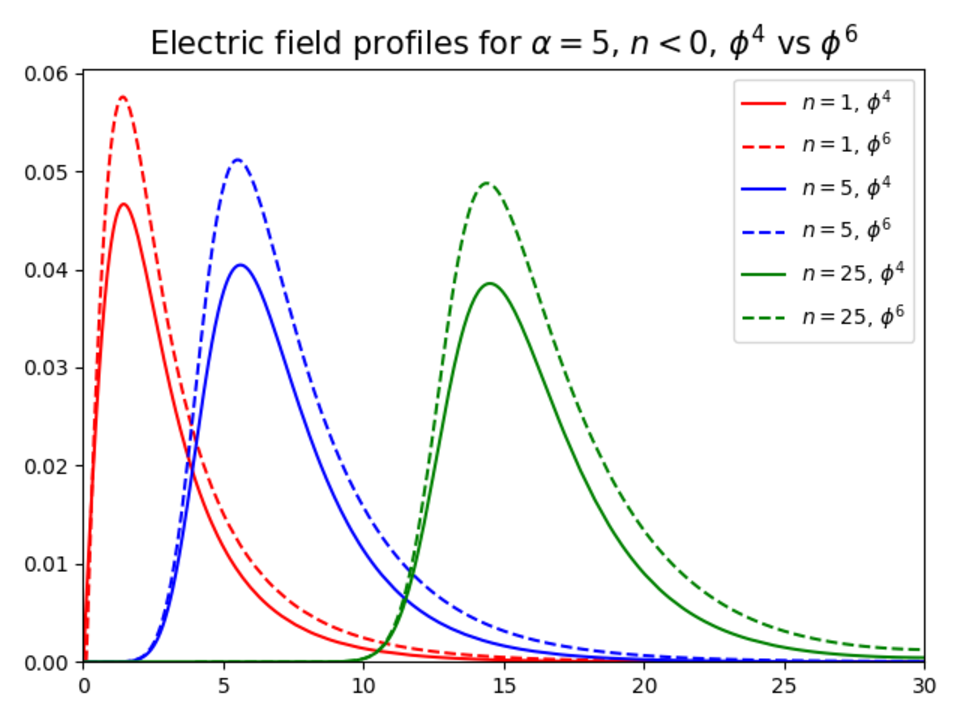
\includegraphics[width=1.85in]{Chapter_2_Folder_1912.11321/figures/E_sixthvsfourth.pdf}
     \caption[\textcolor{red}{This figure shows the vortex profiles with negative winding number for quartic and sextic potentials.}]{{ \small Vortex profiles with negative winding number for quartic(solid) and sextic(dashed) potentials.}} \label{sexticprofile}
    \end{center}
\end{figure}

 \begin{figure}[H]
\begin{center}
 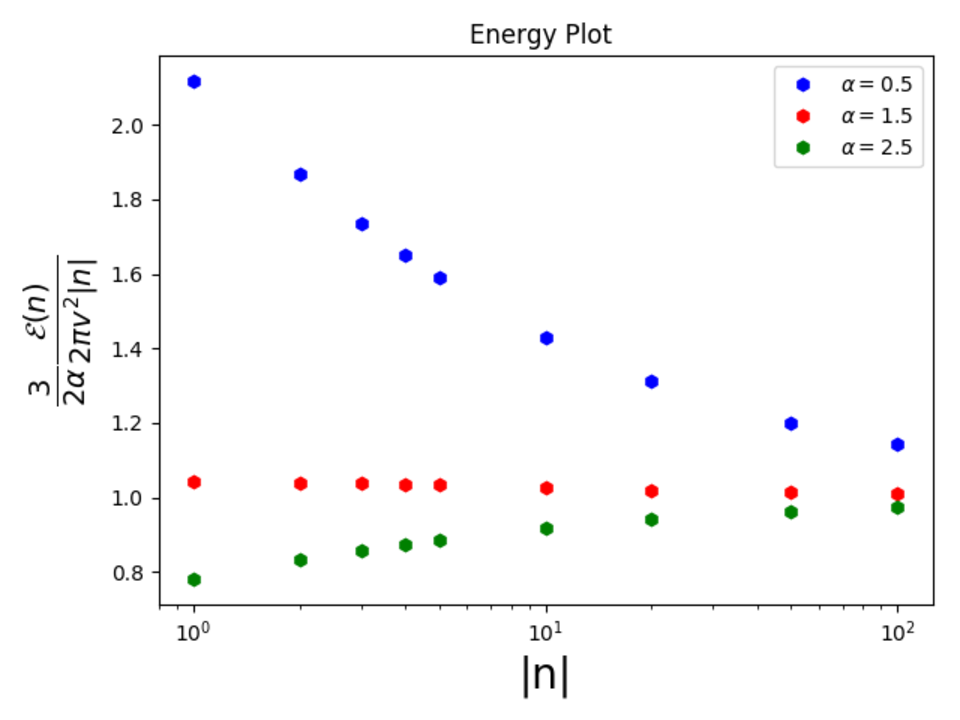
\includegraphics[width=2.8in]{Chapter_2_Folder_1912.11321/figures/sixth_order_alpha.pdf}\hspace{0.1in}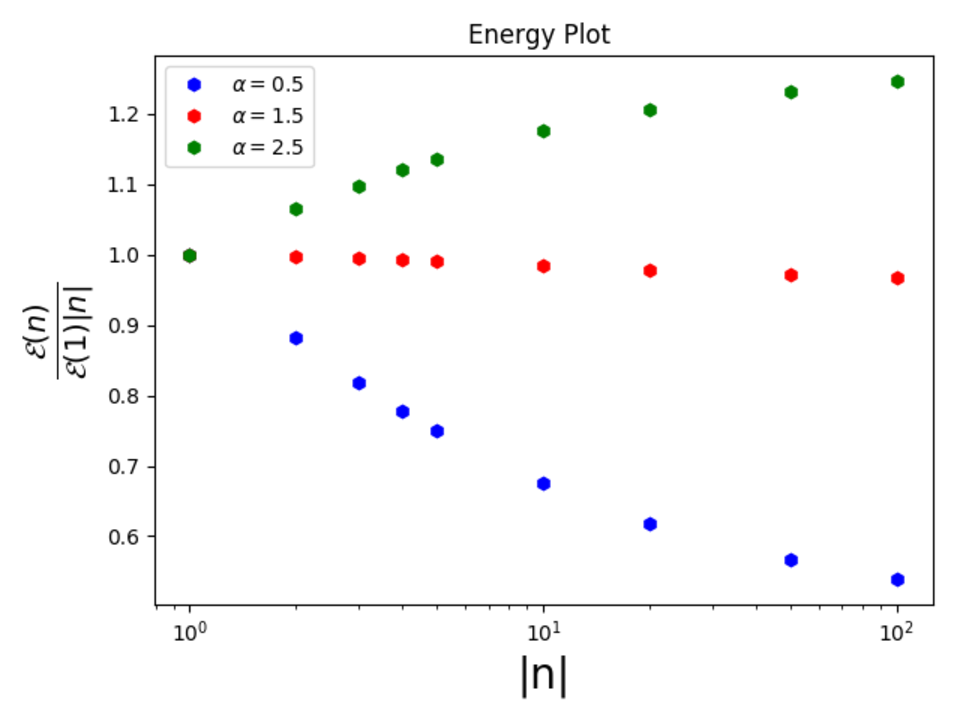
\includegraphics[width=2.8in]{Chapter_2_Folder_1912.11321/figures/sixth_order_alpha_byE1.pdf}
     \caption[\textcolor{red}{This figure shows the scaling of the energy of the $n$-vortex with $|n|$ and $\alpha$, with sextic potential.}]{{ \small The scaling of the energy of the $n$-vortex with $|n|$ and $\alpha$, with sextic potential.}} \label{sexticenergy}
    \end{center}
\end{figure}
The dependence of the energy on $|n|$ and $\alpha$ matches the prediction \eqref{generalenergy}, and we find a transition line between type I and type II vortices at the critical coupling $\alpha_c = \tfrac32$ which represents the marginally bound ``BPS" case for the sextic potential.   Again the value of $\tilde A_0(0)$ indicates that the profiles almost satisfy the first order equation which would imply,
\be
\tilde A_0(0)\,=\,-\frac{1}{2\alpha_c}\,=\,-\frac13\,.
\ee
This is indeed what we observe in figure \ref{A0sextic}. All large $n$ vortex profiles approach this value
\begin{figure}[H]
\begin{center}
    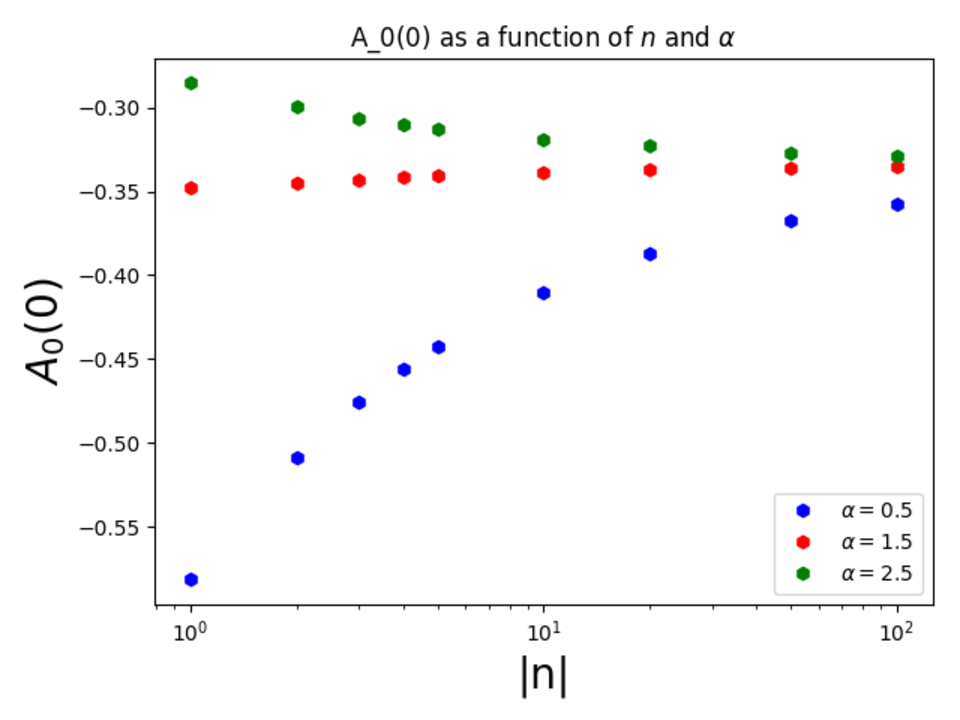
\includegraphics[width=2.9in]{Chapter_2_Folder_1912.11321/figures/sixth_order_A0.pdf}     \caption[\textcolor{red}{This figure shows value of $\tilde A_0$ at the origin for different values of $\alpha$, as a function of $|n|$,  
 with the sextic potential.}]{{ \small Value of $\tilde A_0$ at the origin for different values of $\alpha$, as a function of $|n|$,  
 with the sextic potential.}} \label{A0sextic}
    \end{center}
\end{figure}
\section{Discussion}
We have studied Abelian Chern-Simons vortices in the presence of a chemical potential driving the theory into the Higgs phase. The numerical solutions reveal several features which are in line with the physical picture presented in an analytically solvable (nonrelativistic) supersymmetric model \cite{Tong:2015xaa, Tong:2003vy}.  The configurations with large (negative) flux show precise BPS-like scaling of energy/grand potential and appear (numerically) to closely solve first order equations.
It would be interesting to make use of the large flux limit to understand the edge excitations of the vortex droplet. We expect that some of the lessons learnt from analyzing this system will be of use in $SU(N)$ and $U(N)$ Chern-Simons-scalar theories with a particle number chemical potential. In these theories the ground state putatively breaks rotational invariance due to condensation of vector fields \cite{Kumar:2018nkf}, and depending on whether we are in the $SU(N)$ or $U(N)$ theory, particle number is ungauged or gauged,  and we will have superfluid or superconducting vortices. 

%\acknowledgments We thank Jeff Murugan for discussions on closely related topics. SPK acknowledges support from STFC grant ST/P00055X/1. SS is supported by an STFC studentship under the DTP grant ST/N504464/1.



\chapter{Roton-phonon excitations in Chern-Simons matter theory at finite density}
\label{ch:Chapter_3}
    \graphicspath{{Chapter_3_Folder/figures/PNG/}{Chapter_3_Folder/figures/PDF/}{Chapter_3_Folder/figures/}}

\section{Introduction}
Relativistic field theories in three dimensions consisting of Chern-Simons gauge fields coupled to matter have been conjectured to enjoy a Bose-Fermi/level-rank duality symmetry \cite{Giombi:2011kc}. Mounting evidence for the conjecture has appeared in various forms. These include detailed aspects of  correlators \cite{Giombi:2011kc, Aharony:2011jz, Maldacena:2011jn, Maldacena:2012sf, Aharony:2012nh} and S-matrices \cite{Jain:2014nza, Dandekar:2014era} in large-$N$ vector models coupled to Chern-Simons gauge fields in the 't Hooft limit when the theory  becomes exactly solvable. 
Further, the large-$N$ thermal partition functions have been shown to exhibit Bose-Fermi duality as the 't Hooft coupling is varied \cite{Giombi:2011kc, Aharony:2012ns,Jain:2013py, Jain:2013gza, Takimi:2013zca}.  A crucial role in this is played by the nontrivial eigenvalue distributions of the holonomy matrix around the Euclidean thermal circle, and the duality manifests itself in various phases characterized by the large-$N$ eigenvalue distributions. The  finite $N$ versions of the duality can be precisely formulated \cite{Aharony:2015mjs}, and include an intricate web of abelian dualities \cite{Seiberg:2016gmd, Karch:2016sxi, Murugan:2016zal} with particle-vortex duality as one of its strands.

 In this work, motivated by the goal of understanding the manifestations of Bose-Fermi duality at finite density, we  study the zero temperature ground states of a fundamental scalar coupled to Chern-Simons gauge fields in the presence of a chemical potential for particle number. In particular, we will be mainly interested in finite density ground states in the (semi-)classical limit which spontaneously break the global $U(1)_B$ particle number symmetry. This is a subtle issue in 2+1 dimensions, as any finite temperature will result in thermal fluctuations that, by the Coleman-Mermin-Wagner theorem \cite{Coleman:1973ci, Mermin:1966fe}, can  destroy long-range order. 
 For this reason, in this thesis we limit ourselves to the system at zero temperature. 
 At  non-zero temperature and finite density in the absence of condensates,  exact results at large-$N$ for Chern-Simons theory with a fundamental fermion \cite{Geracie:2015drf, Gur-Ari:2016xff} show nontrivial agreement at strong 't Hooft coupling\footnote{The 't Hooft coupling $\lambda$ is defined in the limit $N,k\to\infty$  ($k$ is the Chern-Simons level) where $\lambda \,\equiv\,\frac{N}{k}$, ranging between $0$ and $1$. } with the weakly interacting bosonic counterpart.
 
 In our analysis of the Chern-Simons-scalar system we  assume a classical limit i.e.  the Chern-Simons level $k$ is large (but finite), and any other scalar self-couplings taken to be  suitably weak so that the semiclassical description applies.  Our main findings are summarized below:
 \begin{itemize}
 \item{We find that the theory with $SU(N)$ gauge group, Chern-Simons level $k$ and non-zero chemical potential for particle number, exhibits a zero temperature ground state where  the scalar field condenses and all gauge fields acquire noncommuting background expectation values.  This ground state breaks the $SU(N)$ gauge symmetry completely and spontaneously breaks the global $U(1)_B$ particle number symmetry. While spatial rotations act nontrivially on the background gauge potentials, they  can be undone by a $U(1)_C$ subgroup of global $SU(N)$ transformations.  Thus gauge invariant operators acquire rotationally  invariant expectation values. The scalar VEV itself is left invariant by a combination of the flavour $U(1)_B$ and global colour $U(1)_C$ rotations. }
 \item{For the $SU(2)$ theory, assuming $k\gg 1$, we obtain the spectrum of physical fluctuations and their dispersion relations in the Bose condensed ground state. The fluctuation spectrum exhibits a massless phonon mode with linear dispersion relation 
 for the frequency $\omega\sim c_s |{\bf k}|$, for low spatial momenta ${\bf k}$, accompanied by a local maximum and a roton minimum at some finite spatial momentum.  Roton-maxon excitations are well known within the context of superfluidity in ${}^4{\rm He}$  \cite{Landau:1941vsj, Schmitt:2014eka} and explain various physical characteristics such as heat capacity and the superfluid critical velocity. The roton minimum, for instance, lowers the superfluid critical velocity to below the speed of sound, as can be understood by applying the Landau criterion \cite{Landau:1941vsj, Schmitt:2014eka}. In the context of this chapter, we understand the appearance of the roton minimum as a consequence of level crossing of states. In the strict limit $k\to \infty$ when the Chern-Simons fields decouple, the interacting scalar theory has a Bose condensate with two gapless excitations at zero momentum, one with quadratic and the other with a linear dispersion relation. At  large but finite $k$, the former acquires a gap at zero momentum, and the putative intersection between the linear and quadratic dispersion curves is replaced by a roton-maxon pair in the diagonalized spectrum. The background VEVs for the gauge fields are directly responsible for these features. Roton-like excitations with very similar origin i.e. constant background gauge fields have been identified in Yang-Mills-Higgs systems at finite density in 3+1 dimensions \cite{Gusynin:2003yu}.
 
 We find that the roton minimum in the phonon dispersion relation persists in the free scalar theory coupled to Chern-Simons gauge fields (at large $k$). In this case the only dimensionful scale is provided by the chemical potential which can be rescaled to unity and the resulting spectra and dispersion relations acquire a universal form.  }
 \item{For the general $SU(N)$ case an interesting picture emerges. The $N\times N$ matrices of VEVs for the Chern-Simons gauge fields provide  finite dimensional versions of harmonic oscillator  creation and annihilation operators. In particular, they can be viewed as the noncommuting coordinates of $N$ particles in a disc of fixed radius. The same matrices have been used to describe the ground state of the quantum Hall droplet \cite{Polychronakos:2001mi, Susskind:2001fb}. Fluctuations about the finite density ground state  may thus be viewed as fluctuations of this droplet (in configuration space), carrying spatial momentum and frequency.}
  \end{itemize}
 The zero temperature finite density properties of the Chern-Simons-scalar system present a range of physical phenomena interesting in their own right. Importantly, they provide predictions for the fermionic dual.  The $SU(N)_k$  theory with a fundamental scalar (and level $k$) is level-rank dual to the $U(k-N)_{-k, -N}$ theory\footnote{The two subscripts denote the Chern-Simons levels of the $SU(k-N)$ and $U(1)$ factors of the gauge group respectively.} with a fundamental fermion \cite{Aharony:2015mjs}. In particular, the free scalar coupled to Chern-Simons fields is dual to the Chern-Simons plus critical fermion theory \cite{Minwalla:2015sca}. It is clearly of great interest to understand whether features of the spectrum of the weakly coupled scalar system can be understood from the conjectured fermionic dual at strong coupling.
 
 This chapter is organized as follows. In section \ref{sec2} we study the Bose condensed ground state of the $SU(2)$ system in the classical limit. In section \ref{sec3} we find the spectrum of quadratic fluctuations after gauge fixing, and identify the phonon-roton branch for different regimes of parameters. Section \ref{sec4} is devoted to the generalization of the classical vacuum structure to general $N>2$.  Finally we outline a number of questions for future study in section \ref{sec5}.
 
  \section{The $SU(2)_k$ theory}
  \label{sec2}
We consider Chern-Simons theory with $SU(2)$ gauge group and one scalar flavour transforming in the fundamental representation. Working with an 
 anti-hermitean gauge potential $A_\mu$, 
\be
A_\mu\,=\,A_{\mu}^{(a)}\,t^a\,,\qquad t^a\,\equiv\,\frac{i}{2}\sigma^a\,,\qquad a=1,2,3\,,
\ee
where $\left\{\sigma^a \right\}$ are the Pauli matrices and $\{A_\mu^{(a)}\}$ are real valued fields,  the Chern-Simons action with (quantized) level $k$ is then,
\be
S_{\rm CS}\,=\,\frac{k}{4\pi}\int d^3x\,\epsilon^{\mu\nu\rho}\,{\rm Tr}\left(A_\mu\partial_\nu A_\rho\,+\,\frac{2}{3}A_\mu A_\nu A_\rho\right)\,.\label{E3}
\ee
This is the action for both Euclidean $(+++)$ and Lorentzian $(-++)$ signatures. The Wick rotation  from Lorentzian to Euclidean is implemented by the replacement $t\to -i\tau$ and $A_0 \to i A_0$, which together leave $S_{\rm CS}$ invariant.  In Lorentzian signature, the complete action involving Chern-Simons and matter fields has the general form,
\be
S\,=\,S_{\rm matter}\,+\, S_{\rm CS}\,,
\ee
where, in Lorentzian signature $(-++)$, for a scalar $\Phi$ transforming in the fundamental representation of $SU(2)$,
\bea
&&\,S_{\rm matter}\,=\,-\int d^3x\left(\left(D_\mu\Phi\right)^\dagger\left(D^\mu\Phi\right)\,+\,V(\Phi^\dagger \Phi)\right)\,,\label{E4}\\\nonumber\\\nonumber
&& D_\mu\,\equiv\,\partial_\mu\,+\,A_\mu\,.
\eea
The theory possesses a {\em global} $U(1)$ symmetry which we refer to as  ``baryon number" or $U(1)_B$,
\be
U(1)_B:\qquad \Phi\,\to\,e^{i\vartheta}\,\Phi\,,
\ee
generated by a phase rotation of $\Phi$. The corresponding conserved current is 
\be
j^\mu_B\,=\,i\,\left[\left(D^\mu\Phi\right)^\dagger \Phi\,-\,\Phi^\dagger D^\mu\Phi\right]\,.
\ee
The chemical potential $\mu_B$ is a Lagrange multiplier for the $U(1)_B$ charge. In Lorentzian signature, it therefore appears in the Lagrangian as a time component for a background $U(1)_B$ gauge field:
\be
D_\nu\,\to\, D_\nu\,+\,i\mu_B \,\delta_{\nu,0}\,.
\ee
\subsection{Classical ground states with $\mu_B\neq 0$}
The coupling of the Chern-Simons fields to the matter sector is controlled by $1/\sqrt{k}$\,\footnote{This can be understood via the rescaling $A_\mu \to A_\mu/\sqrt{k}$, following which the Chern-Simons action is order $1$ in the large $k$ limit.}. 
In the limit $k\to \infty$, the scalar field $\Phi$ with $\mu_B\neq 0$ has the potential:
\be
V_{\rm scalar}(\mu_B,\,k\to\infty)\,=\,V(\Phi^\dagger\Phi)\,-\,\mu_B^2\,\Phi^\dagger\Phi\,.
\ee
As usual, the effective negative mass squared due to the chemical potential drives the system to form a Bose condensate for large enough $\mu_B$. The tree level 3D scalar potential (at $\mu_B=0$) can be taken to  be of the form,
\be
V(\Phi^\dagger\Phi)\,=\,m^2\,\Phi^\dagger\Phi\,+\,g_4(\Phi^\dagger\Phi)^2\,+\,g_6\,(\Phi^\dagger\Phi)^3\,,
\ee
where we have allowed for relevant and marginal operators in the scalar potential.
Assuming that the ground state of the theory with $\mu_B\neq 0$ is static and translation invariant, we look for vacuum solutions with all terms involving derivatives being set to zero.  Anticipating a scalar condensate at the classical level\footnote{The analysis will remain purely classical and at zero temperature at this stage. At finite temperature, we know that quantum thermal fluctuations in 2+1 dimensions preclude symmetry breaking of continuous global symmetries.}, we can always choose gauge rotations to take the VEV to be real and of the form, 
\be
\langle\Phi\rangle\,=\,\left(
\begin{matrix}
 0 \\ v
\end{matrix}
\right)\qquad v\in {\mathbb R}\,.
\ee
We then collectively view all non-derivative terms as potential energy contributions:
\bea
V_{\rm CS}\,+\,V_{\rm scalar}&&=\,-\frac{k}{4\pi}\epsilon^{\mu\nu\rho}A_\mu^{(1)}\,A_\nu^{(2)}\,A_\rho^{(3)}\,-\, \frac{v^2}{4}\left[\left(A_0^{(1)}\right)^2 \,+\,\left(A_0^{(2)}\right)^2\,+\,\left(A_0^{(3)}\, -\,2\mu_B\right)^2\right]\nonumber\\
\label{potential}\\\nonumber
&&+\, \frac{v^2}{4}\sum_{i=1,2}\left[\left(A_i^{(1)}\right)^2 \,+\,\left(A_i^{(2)}\right)^2\,+\,\left(A_i^{(3)}\right)^2\right]\,+\,m^2\,v^2\,+\,g_4\,v^4\,+\,g_6\,v^6\,.
\eea
One consistent extremum is given by $v=0$, and all gauge fields also vanishing. This is the trivial solution. However, this solution cannot dominate the grand canonical ensemble for generic values of the chemical potential. In particular,  the scalar field theory without Chern-Simons terms ($k^{-1}\to 0$),  and at weak coupling  $(g_{4}\ll m, g_6\ll 1)$,  develops a Bose condensate when $|\mu_B| >  m$.   This non-trivial phase with $v\neq 0$ must persist when the coupling to Chern-Simons gauge fields is turned on. 
In order to arrive at a static and translationally invariant ground state, we need to find the minima of the potential energy function \eqref{potential}. We adopt a notation which is appropriate for $SU(2)$ by introducing three-vectors in the internal ``isospin" directions:
\be
{\bf A}_{\mu}\,\equiv\,\left(\langle A_\mu^{(1)}\rangle,\,\langle A_\mu^{(2)}\rangle,\,\langle A_\mu^{(3)}\rangle \right)^{ T}\qquad 
{\bf e}^{a}\,\equiv\,\left(\delta^{a,1},\,\delta^{a,2},\,\delta^{a,3}\right)^T\,.
\ee
In terms of these, the vacuum equations determining the ground state are (here the `$\times$' and `$\cdot$' symbols denote cross- and dot-products in the internal space):
\begin{eqnarray}
&& v^2 {\bf A}_y\,=\,\frac{k}{2\pi}{\bf A}_0\times{\bf A}_x\,,\qquad v^2 {\bf A}_x\,=\,\frac{k}{2\pi}{\bf A}_y\times{\bf A}_0\,,\label{eq1}\\\nonumber\\
&& -v^2\left({\bf A}_0-2\mu_B {\bf e}^3\right)\,=\,\frac{k}{2\pi}{\bf A}_x\times{\bf A}_y\,,\label{eq2}\\\nonumber\\
&&\frac{v}{2}\left[\left({\bf A}_0-2\mu_B {\bf e}^3\right)^2-\left({\bf A}_x\right)^2-\left({\bf A}_y\right)^2\right]\,=\,\frac{\partial V}{\partial v}\,.\label{eq3}
\end{eqnarray}
The  two equations in \eqref{eq1} together imply that ${\bf A}_0, {\bf A}_x$ and ${\bf A}_y$ are mutually orthogonal in the internal isospin directions, and that
\be
\left|{\bf A}_x\right|\,=\,\left|{\bf A}_y\right|,\qquad \left|{\bf A}_0\right|\,=\,\frac{2\pi v^2}{|k|}\,\,,\qquad {\rm sgn}\left[\left({\bf A}_x\times {\bf A}_y\right) \cdot{\bf A}_0\right]\,=\,{\rm sgn}(k)\,.
\ee
Next, by taking a cross-product of \textcolor{red}{equation} \eqref{eq2} with ${\bf A}_0$, we deduce that ${\bf A}_0\,=\, \langle A_0^{(3)}\rangle  {\bf e}^3$:
\begin{align}
    \textcolor{red}{   \left({\bf A}_x\times{\bf A}_y\right)\times{\bf A}_0\,}&\textcolor{red}{=\,{\bf A}_y \big( {\bf A}_0 \cdot {\bf A}_x \big)\, -\, {\bf A}_x \left({\bf A}_0 \cdot {\bf A}_y\right)}\nonumber\\
    &\textcolor{red}{= \frac{k}{2\pi v^2} \bigg({\bf A}_y \underbrace{ \big( {\bf A}_0 \cdot \big({\bf A}_y \times {\bf A}_0\big) \big)}_{=0}\, -\, {\bf A}_x \underbrace{\left({\bf A}_0 \cdot  \big({\bf A}_0 \times {\bf A}_x\big) \right) }_{=0}\bigg) =\,0}\nonumber\\
    &\textcolor{red}{\implies\, {\bf A}_0 \times {\bf e}^3\,=\,0\,,}
\end{align}
 \textcolor{red}{where we have used (\ref{eq1}) in the second line.}
Finally, combining equations \eqref{eq2} and \eqref{eq3}, we obtain conditions on the magnitudes of the background field expectation values:
\bea
&&\left|{\bf A}_x\right|^2\,=\,\left|{\bf A}_y\right|^2\,=\,\frac{2\pi v^2}{|k|}\left|\langle {A}_0^{(3)}\rangle\,-\,2\mu_B \right|\\\nonumber\\
&& \left(\langle {A}_0^{(3)}\rangle\,-\,2\mu_B\right)^2\,-\,\frac{4\pi v^2}{|k|}\left|\langle{A}_0^{(3)}\rangle\,-\,2\mu_B \right|\,-\,\frac{2}{v}\frac{\partial V}{\partial v}\,=\,0\,.\label{vaceq}
\eea
%For a convex scalar potential function, this immediately leads to the restriction,
%\be
%\left|\langle {A}_0^{(3)}\rangle\,-\,2\mu_B \right| \,>\,\frac{4\pi v^2}{|k|}\,.
%\ee
To proceed further, it is useful to work with the (isospin) basis elements
\bea
&&{\bf A}_0\,=\,\eta \frac{2\pi v^2}{|k|} {\bf e}^3\,,\qquad{\bf A}_x\,=\, a_1\,{\bf e}^1 \,+ \,a_2 \,{\bf e}^2\,,\qquad
{\bf A}_y\,=\, \eta\, {\rm sgn}(k)\,\left(-a_2\,{\bf e}^1\, +\, a_1 \,{\bf e}^2\right)\,,
\nonumber
\eea
where $\eta \,=\,\pm 1$ and $a_{1,2}\in {\mathbb R}$. Using the equations of motion \eqref{eq1} and \eqref{eq2} we then find that
\be
 \eta \,=\,{\rm sgn}(\mu_B)\,, \qquad (a_1)^2\, +\, (a_2)^2\,=\,\frac{4\pi v^2}{|k|}\left(|\mu_{B}| -\frac{v^{2}\pi}{|k|}\right)\,,\qquad   |\mu_B| > \frac{\pi v^2}{|k|}\,.
 \label{E14} 
 \ee
 The classical configuration is endowed with a non-zero $U(1)_B$ charge density,
 \be
\langle j^0_B\rangle\,=\,{\rm sgn}(\mu_B) \frac{2\pi v^4}{|k|}\,,
 \ee
 with vanishing $U(1)_B$ currents.
 To calculate the scalar VEV we need the form of the tree level potential. For simplicity we set $g_6=0$. With a quartic potential there exists a unique solution\footnote{The second root for $v^2$ yields $v^2 >|\mu_B k|/2\pi$ and violates the condition in eq. \eqref{E14}.} for the vacuum expectation value \eqref{vaceq},
 \be
 v^2 = \frac{|k|}{3\pi} \left( \frac{g_4 |k|}{\pi} + {2 |\mu_{B}|} - \sqrt{ \left(\frac{g_4 |k|}{\pi} + {2 |\mu_{B}|}\right)^2\,-\,3( \mu_{B}^2 -m^2)
 %+ \frac{g_4^2k^2}{\pi^2} + \frac{4g_4}{ \pi}  |\mu_{B} k|   
 } \right)\label{VEV}\,,
 \ee
 which also satisfies the condition \eqref{E14}. As expected, the VEV is real only when $\mu_B^2 > m^2$, and in the large $k$ limit when the Chern-Simons gauge fields decouple, $v^2 \simeq (\mu_B^2-m^2)/2 g_4$. This is, of course, the scalar VEV in the pure scalar theory in the Bose condensed phase. In the massless theory, the scalar VEV is controlled by the dimensionless combination $|\pi \mu_B/g_4k|$:
 \bea
 m=0:\qquad &&v^2\,=\,\frac{|\mu_B k|}{2\pi}\,f(\tilde\mu)\,,\qquad \tilde\mu\,\equiv\,\frac{\pi |\mu_B|}{g_4 |k|}\\\nonumber\\\nonumber
 && f(\tilde\mu)\,=\,\frac{2}{3} \left(\tilde\mu^{-1}+2 -\sqrt{(\tilde\mu^{-1}+2)^2-3}\right)\,,
 \eea
 where $f(\tilde \mu)$ is  monotonically increasing with $f(0)=0$ and $f(\infty)\simeq \frac{2}{3}$. A noteworthy point here is that the scalar VEV exists even when $g_4$  technically vanishes.  More generally, one may view the semiclassical limit in which the condensate is well defined as  $(g_4/\mu_B)\to 0$ and $k\to\infty$ such that $g_4 k/\mu_B$ is kept fixed.
 
 \paragraph{Free energy:} For static configurations  we can compute the free energy density by evaluating the potential energy function on the ground state.   In terms of the VEV, the free energy is,
 \be
F \,=\, v^2\left[g_4v^2 +m^2 - \left(|\mu_B|-\frac{\pi v^2}{k}\right)^2\right]\,.
 \ee
 It is easy to check that (assuming $|\mu_B| > m$) the function is negative definite.
 In the massless case, the free energy of the Bose condensed phase is determined by the function $f(\tilde\mu)$:
 \be
 F\left.\right|_{m=0}\,=\,\frac{|\mu_B^3 k|}{4\pi} \frac{f(\tilde\mu)}{\tilde\mu}\left[f(\tilde\mu)-\tfrac{\tilde\mu}{2}\left(f(\tilde\mu)-2\right)^2\right]\,,
 \ee
 which is a negative definite, monotonically decreasing function of $\tilde\mu$. Therefore, in the semiclassical regime, the nontrivial vacuum dominates over the trivial one with vanishing VEVs for all fields. For instance, in the massless theory with $g_4=0$, the free energy in the Higgsed phase is
 \be
 F\left.\right|_{m=0,g_4=0}\,=\,-4\frac{|\mu_B^3 k|}{27\pi}\,,
 \ee
  valid in the semiclassical limit $k\gg 1$. Quantum corrections are parametrically suppressed in this limit. In this case the theory enters the Higgsed phase for any non-zero chemical potential, while the theory with vanishing chemical potential is conformal.   When the mass is non-zero and the chemical potential is dialed past the classical threshold value $\mu_B=m$, following a second order phase transition, the theory enters a Bose condensed Higgs phase.   The symmetric phase is unstable beyond this point. This interpretation is supported by the plot (figure \ref{fvsv}) of the free energy as a function of the VEV $v$ (taking $g_4=0$ for simplicity).
   \begin{figure}[h]
\begin{center}
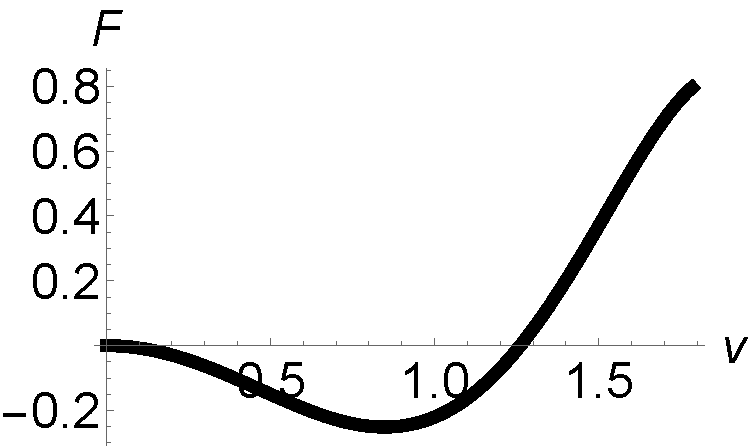
\includegraphics[width=2in]{Chapter_3_Folder_1806.06976/figures/Fvsv.pdf}
\end{center}
%\includegraphics[width=0.55\textwidth]{Dispersion_Relations}
%\includegraphics[width=0.45\textwidth]{Critical_velocity}
       \caption[This figure shows the effective potential (free energy density) as a function of the VEV $v$ for $\mu_B=1$, $m=0.5$ and $g_4=0$.
]{ The effective potential (free energy density) as a function of the VEV $v$ for $\mu_B=1$, $m=0.5$ and $g_4=0$.
}
\label{fvsv}
\end{figure}
The effect of  quantum corrections at large $k$ will be to renormalize the mass  in the symmetric phase and change the threshold value of the chemical potential at which the (second order) phase transition from the symmetric to the Higgsed phase occurs. This qualitative picture may change for finite $k$ when quantum corrections are large.

 \subsection{Colour-flavour locked symmetry}
 We have found a one-parameter family of gauge field solutions parametrised by the variables $(a_1, a_2)$, satisfying a constraint \eqref{E14}. Any given realization breaks the $SU(2)$ gauge symmetry completely due to the scalar VEV which also breaks $U(1)_B$. However, the scalar VEV is left invariant by the diagonal combination of $U(1)_B$ and a  $U(1)$ subgroup of the {\em global}  $SU(2)$ colour rotations:
 \be
U(1)_B:\, \langle \Phi\rangle \,\to\,e^{i\vartheta/2} \langle \Phi\rangle \,\qquad U(1)_C:\,\Phi\,\to\,U(\vartheta)\Phi\,,\qquad U(\vartheta)\,\equiv\,e^{i\vartheta\sigma_3/2}
 \ee
While the gauge fields do not transform under $U(1)_B$, they do transform under the global $U(1)_C$ . The transformation acts on the background gauge fields $\langle A_i\rangle \,=\,\langle A_i^{(a)}\rangle t^a$ exactly as a rotation $(R)$ by a constant angle $\vartheta$ in the $x$-$y$ plane:
\bea
U(1)_C:\, \left(\begin{matrix}
\langle A_x\rangle \\ \langle A_y\rangle
\end{matrix}\right)
 \,\to\,  \left(\begin{matrix}  U(\vartheta)\langle A_x\rangle U^\dagger(\vartheta) 
\\ \\  U(\vartheta)\langle A_y\rangle U^\dagger(\vartheta)\end{matrix}\right)
 \,=\,\left(\begin{matrix} \cos \vartheta \, & \quad-\sin \vartheta
 \\\sin \vartheta\,&\quad\cos \vartheta \end{matrix}\right )
 \left(\begin{matrix} \langle A_x\rangle \\ \langle A_y\rangle \end{matrix}\right ),
 %\quad  U(\theta)\,\equiv\,e^{i \theta\sigma_3}.\nonumber
%&& A_y \,\to\,  e^{i\alpha\sigma_3} A_y  e^{-i\alpha\sigma_3}\,=\, \sin (2\alpha)\,A_x\,+\,\cos(2\alpha) \,A_y\,.
\label{rotmatrix}
\eea
Therefore the vacuum gauge configuration is invariant under a global $U(1)_{B+C+R}$ symmetry which can be viewed as a  linear combination of global colour, flavour (or baryon number) and $SO(2)$ rotations in the $x$-$y$ plane.

The above observation has an important consequence. It implies that the ground state does {\em not} actually break rotational invariance\footnote{This will be corroborated by the spectrum of physical fluctuations which we extract subsequently.}, since the action of  rotations can be undone by  a gauge transformation. This is naturally reflected in the expectation values of all gauge invariant operators built from field strengths. In particular, the expectation values of single trace operators built from the chromoelectric and chromomagnetic field strengths are independent of the spatial direction or spatial component in question:
\be
\langle{\rm Tr}\left( F_{0i}\right)^{2}\rangle\,=\,-\tfrac{2\pi^3 v^6}{|k|^3}\left(\mu_B-\tfrac{v^2\pi}{|k|}\right)\,,\qquad \langle{\rm Tr}\left( F_{ij}\right)^{2}\rangle\,=\,-\tfrac{8\pi^2 v^4}{|k|^3}\left(\mu_B-\tfrac{v^2\pi}{|k|}\right)^2\,.
\ee

%However, we need to find a nontrivial minimum with $v\neq 0$ which is the correct generalisation of the $k\to\infty$ scalar condensate to finite values of $k$. This is obtained by solving the equation,
%\be
%4 g_4\,v^2\,+\,2m^2\,-\,\frac{v}{2}\left(A_0^{(3)}-2\mu_B\right)^2
%\,+\,\frac{4\pi}{k}\frac{v^2}{2}\left(A_0^{(3)}-2\mu_B\right)\,=\,0\,.
%\ee
%Note that in the strict $k\to\infty$ limit (keeping $v$ fixed), we have $A_0^{(3)}\to 0$, the VEV is solved by the standard classical condensate $v^2\,=\,(\mu_B^2-m^2)/2g_4$. Away from this limit, the above equation is a quadratic equation in $v^2$ and can be solved quite easily in order to obtain the most general solution with non zero VEV,
%\begin{eqnarray}
%v_{\pm}^2 = \frac{1}{3} \left( \frac{g_4 k^2}{\pi^2} + \frac{2 |\mu_{B} k|}{\pi} \pm \frac{|k|}{\pi^2} \sqrt{g_4^2 k^2 + 4 \pi g_4 |\mu_{B} k| + \pi^2 \mu_{B}^2 + 3m^2 \pi^2} \right)\label{E13}
%\end{eqnarray}
%together with the gauge fields,
%\begin{eqnarray}
%A_x^3 &=& A_0^1= A_y^3=A_0^2 = 0,\nonumber\\
%A_x^2 &=& sgn(\mu_{B} k) A_y^1, ~A_x^1  = -sgn(\mu_{B} k) A_y^2, \nonumber\\
%A_0^3 &=& sgn(\mu_{B} k) \frac{2 \pi v^2}{|k|},~(A_{x}^{2})^{2}+(A_{x}^{1})^{2}=\frac{4 \pi v^{2}}{|k|}\left(|\mu_{B}| -\frac{v^{2}\pi}{|k|}\right).\label{E14} 
%\end{eqnarray}
%One immediate observation that directly follows from (\ref{E14}) is the fact that in order to keep the positive norm square for the gauge fields, the corresponding $ U(1)_{B} $ potential must satisfy the following lower bound,
%\begin{eqnarray}
%|\mu_{B}| \geq \frac{v^{2}\pi}{|k|}.\label{e15}
%\end{eqnarray}
%However, it is in fact quite trivial to check that one of the solutions in (\ref{E13}) is in fact inconsistent with the bound (\ref{e15}) mentioned above and therefore the only consistent solution remains to be,
%\begin{eqnarray}
%v^{2}_{-}\equiv v^{2}= \frac{1}{3} \left( \frac{g_4 k^2}{\pi^2} + \frac{2 |\mu_{B} k|}{\pi} - \frac{|k|}{\pi^2} \sqrt{g_4^2 k^2 + 4 \pi g_4 |\mu_{B} k| + \pi^2 \mu_{B}^2 + 3m^2 \pi^2} \right).\label{e16}
%\end{eqnarray} 
 %We thereby identify (\ref{e16}) as the true condensate that triggers the superfluidity at zero temperature.
%Before we proceed further, it is worth mentioning the original symmetries (associated with the ground state prior to the symmetry breaking) and the symmetry breaking effects in the presence of the non zero condensate ($ v $). The non zero condensate in the symmetry broken phase clearly breaks the color $ SU(2)_{c} $ as well as the \textit{global} $ U(1)_{B} $ that we had started with. The color $ SU(2)_{c} $ breaks to nothing. The breaking of the global $ U(1)_{B} $ triggers the so called Goldstone modes in the system. However, it is quite instructive to check that the ground state still preserves 2D rotational invariance. This can be seen in the form of the components of the non-abelian strength tensor,
%\begin{eqnarray}
%det F_{0i} & =& -  \frac{4\pi^ 2v^4}{k^2} ( (A_1^1)^2 +(A_2^1)^2 ) \nonumber \\
%det F_{12} & =&  (A_1^1)^2 +(A_2^1)^2.\label{e17}
%\end{eqnarray}

%Why rotational invariance is not broken is not quite as clear as shown here. If one were to perform a rotation on the gauge fields, the non-abelian field strength components $F_{\mu \nu}$ change. The relevant ($F_{12}$ is explicitly rotationally and gauge invariant) components of the field strength are

%\begin{align}
%F_{01} &= sgn (\mu_{B} k) \frac{\pi v^2}{2|k|}\left(\begin{matrix}
%& \ 0 \ & \ A_1^2+i A_1^1 \\ & \ A_1^2 -i A_1^1 \ & \ 0 
%\end{matrix}\right) \nonumber \\
%F_{02} &= sgn (\mu_{B} k) \frac{\pi v^2}{2|k|} \left(\begin{matrix}
%& 0 \ & -A_1^1+i A_1^2 \\ & -A_1^1 -i A_1^2~ \ & 0 
%\end{matrix}\right).
%\end{align}
%We can see that performing either a rotation or a gauge transformation separately, changes the field strength tensor. However, we see that there is a residual abelian symmetry leftover by doing the following transformation, which is a certain composition of $U(1)_B$ global, SO(2) and the third ($\sigma^3$) generator of $SU(2)_c$:
%\begin{align}
%\Phi & \xrightarrow{SU(2)_c} e^{i \theta \sigma^3} \Phi \nonumber \\
%\Phi & \xrightarrow{U(1)_B} e^{i \theta} \Phi \nonumber \\
%A_{\mu}^a & \xrightarrow{SO(2)} R_{\mu}^{\ \nu}(\theta)A_{\nu}^a \nonumber \\
%F_{\mu \nu} & \xrightarrow{SU(2)_c} U(\theta) F_{\mu \nu} U(\theta)^{\dagger},
%\end{align}
%where $U(\theta)= e^{i \frac{\theta	}{2} \sigma^3}$.
\section{Spectrum of fluctuations}
\label{sec3}
We now turn to the spectrum of quadratic fluctuations about the classical vacuum configuration. In the quantum theory this is reliable at weak coupling i.e. $k\gg 1$ and $\mu_B\gg g_4$. \textcolor{red}{The masses and dispersion relations derived in this section follow the technique described in Section 2.2.1 and so precise details into the derivations will be omitted from here on.}
\subsection{The $k\to\infty$ theory} 
It is useful to first recall the situation when the Chern-Simons fields are decoupled in the limit $k\to \infty$. In this limit we have a pure scalar field theory with a global $O(4)\supset SU(2)\times U(1)_B$ symmetry. A large enough chemical potential for $U(1)_B$ leads to Bose condensation via  the scalar VEV,
\be
k\to\infty: \quad v^2 \,=\,\frac{\mu_B^2- m^2}{2 g_4}\,, 
\ee
 and the weak coupling spectrum  is readily obtained after diagonalizing the matrix of quadratic fluctuations. There are four physical excitations corresponding to the four real scalar degrees of freedom with the following dispersion relations for the frequency $\omega$ as a function of the spatial momentum ${\bf p}$, where we have set $m=0$ for simplicity:
 \bea
&& \omega^2_{{\rm I}\,(\pm)}\,=\,{\p}^2 + 3\mu^2_B\pm\mu_B\sqrt{4\p^2+9\mu^2_B}\,,\\\nonumber
\\\nonumber
 && \omega^2_{{\rm II}\,(\pm)}\,=\,{\p}^2 + 2\mu^2_B\pm 2\mu_B\sqrt{\p^2+\mu^2_B}\,.
 \eea
Two of these states are gapless\footnote{The chemical potential picks out a  $U(1)_B\simeq SO(2)\subset O(4)$ and breaks the symmetry to $SO(3)\simeq SU(2)$. The scalar condensate spontaneously breaks both the $SU(2)$ and the $U(1)_B$, and the number of Goldstone bosons is lesser than the number of broken generators, as expected  when relativistic invariance is absent \cite{Nielsen:1975hm, Watanabe:2012hr}.}. Of the two, only one has a linear dispersion relation at low momentum and corresponds to the phonon mode while the other has a quadratic dependence on the spatial momentum,
 \be
 \omega_{{\rm I}(-)}\,=\,\frac{|\p|}{\sqrt 3}+\ldots\,,\qquad  \omega_{{\rm II}(-)}\,=\,\frac{\p^2}{2\mu_B}\,+\ldots
 \ee
%\bea
%\eea
The presence of the second gapless mode with quadratic dependence on momentum implies that the Bose condensed ground state cannot be viewed as a 
superfluid, due to vanishing critical velocity according to the Landau criterion \cite{Landau:1941vsj, Schmitt:2014eka}. This picture undergoes a qualitative change  for finite large $k$. 

\subsection{Finite, large $k$}  
For any finite value of $k$, the Chern-Simons gauge fields  couple to the scalars. However, since the gauge fields are non-dynamical, the number of physical degrees of freedom remains unaltered and is given by the number of real scalars. To calculate the semiclassical spectrum we expand  in  fluctuations about the gauge and scalar VEVs,
\begin{eqnarray}
&&A_{\mu}\,=\,\langle{A}_{\mu}\rangle\,+\,{\cal A}_{\mu}\,,\qquad 
\Phi\,=\,\langle\Phi\rangle\,+\,{\delta \Phi}\,,\qquad\delta\Phi\,\equiv\,
\ \left(
\begin{matrix}
 \varphi_{1}+i \varphi_{2} \\ \,\varphi_{3}+i \varphi_{4}
\end{matrix}
\right)\,,\label{E17}
\end{eqnarray}
where $ {\cal A}_{\mu}$  and $\{\varphi_i\}$  $(i=1,\ldots 4)$ are respectively, the gauge field  and matter  fluctuations.  Substituting these into the original action \eqref{E3} and  \eqref{E4}, and expanding to quadratic order in fluctuations, 
\bea
{\cal L}^{(2)}\,=&&\delta\Phi^\dagger\,{\cal D}_\mu {\cal D}^{\mu} \,\delta\Phi\,+\, \langle\Phi^\dagger\rangle {\cal A}_\mu {\cal D}^\mu \delta\Phi - {\cal D_\mu}\delta\Phi^\dagger {\cal A}_\mu \langle\Phi\rangle +\langle\Phi^\dagger\rangle {\cal A}_\mu {\cal A}^\mu \langle\Phi\rangle\nonumber \\
+&&\frac{k}{4\pi}\epsilon^{\mu\nu\lambda} {\rm Tr}\left({\cal A}_\mu {\cal D}_\nu{\cal A}_\lambda\right) \,-\,\frac{1}{2}\varphi_j\,\varphi_k \left\langle\frac{\partial^2 V}{\partial \varphi_j\partial \varphi_k}\right\rangle \,.
\eea
Here ${\cal D}_\mu$ denotes the covariant derivative with respect to the background gauge field $\langle A_\mu\rangle$:
\bea
{\cal D}_\mu \delta\Phi\,\equiv\,\partial_\mu\delta\Phi + \left(\langle A_\mu\rangle\,+\,i\mu_B\delta_{\mu,0} \right)\delta\Phi\,,\qquad {\cal D}_\mu {\cal A}_\nu\,\equiv\,\partial_\mu {\cal A}_\nu\,+\,[\langle A_\mu\rangle, {\cal A}_\nu]\,.
\eea
The main point to note here is that in the presence of the VEV for both scalars and gauge fields, all the fluctuations (matter and gauge) couple to each other at quadratic order. Due to the mixings, the physical degrees of freedom and their dispersion relations are not immediately obvious. In order to extract these, we first need to gauge-fix the action for the quadratic fluctuations.  The gauge-{\em unfixed} action would yield a degenerate matrix with vanishing determinant. In the presence of background gauge fields and symmetry breaking scalar VEVs, it is natural to adopt an $R_{\xi}$ gauge which is covariant with respect to the non-zero background gauge fields:
\bea
{\cal L}^{(2)}\,\to\, {\cal L}^{(2)} \,+\, {\cal L}_{\rm gf}\,,\qquad 
{\cal L}_{\rm gf}\,=\,\frac{1}{2\xi}{\rm Tr}\left({\cal D}_\mu{\cal A}^\mu\,-\xi \langle\Phi\rangle \delta\Phi^\dagger \,+\,\xi \delta\Phi \langle\Phi^\dagger\rangle  \,\right)^2.
\eea
The $R_{\xi}$ gauge above removes the derivative couplings between the would-be Goldstone modes and the gauge field fluctuations ${\cal A}_\mu$, and introduces a non-trivial mass matrix for them.

The determinant of the gauge-fixed fluctuation matrix then exhibits zeroes with both $\xi$-dependent and $\xi$-independent dispersion relations. The latter correspond to the physical states of the theory. In fact, these can be isolated by identifying the leading term in the large-$\xi$ expansion of the determinant of fluctuations at fixed frequency and momentum.
\subsubsection{Physical states}
We have checked numerically that the physical states inferred from the procedure above are indeed $\xi$-independent. For the $SU(2)$ theory there are precisely four physical states corresponding to the  two complex components of the scalar doublet, since the  Chern-Simons gauge fields cannot contribute any additional physical, propagating degrees of freedom. The dispersion relations for these four physical states are given by the solutions to a quartic equation in $(\omega^2, {\bf p}^2)$,
\be
\omega^8\,+\,\mu^2_BC_3\,\omega^6\,+\,\mu^4_BC_2 \,\omega^4 \,+\,\mu^6_BC_1\, \omega^2 \,+\,\mu^8_B\, C_0\,=\,0\, \textcolor{red}{,}\label{det}
\ee
where the $\{C_i\}$ $(i=0,\ldots3)$ are functions of dimensionless variables,
\be
C_i\,=\, C_i\left(\frac{{\bf p}^2}{\mu^2_B},\,\frac{g_4}{\mu_B},\,\frac{m^2}{\mu_B^2},\,k\right)\,,
\ee
whose explicit forms are given in \eqref{ci}. 
\paragraph{ The phonon mode:} We first recall that the $U(1)_B$ global symmetry is spontaneously broken and the corresponding Goldstone mode is the phonon. Since the remaining broken symmetries are local, the phonon should be the only massless state. This is confirmed by solving for the spectrum using \eqref{det} at ${\p=0}$ which yields\footnote{We follow the branches with the same nomenclature used for the $k=\infty$ theory. The subscripts ${\rm I}(-)$ and ${\rm II}(-)$ refer to the gapless states in that theory with linear and quadratic dispersion relations, respectively.}
\bea
{\bf p=0:}\quad&&\omega_{{\rm I}-}\,=\,0\, \qquad \qquad
\omega_{{\rm I}+}\,=\,\sqrt{m^2+6g_4v^2 -\mu_B^2 +\left(2|\mu_B|-\frac{\pi v}{|k|}\right)^2}\,,\nonumber\\\\\nonumber
&& \omega_{{\rm II}(-)}\,=\,\frac{4\pi}{|k|}\,v^2 \qquad\qquad \omega_{{\rm II}(+)}\,=\, 2|\mu_B|\,.
\eea
As expected the gapless mode with a quadratic dispersion in the $k=\infty$ theory is lifted. It is then straightforward to find the velocity of the phonon mode. In the limit of small $\omega$ and $|\p|$ we identify the coefficients of the terms quadratic in $\omega$ and $\p$ in the polynomial \eqref{det}. The resulting speed of sound  is then,
\bea
&& c_s\,=\,\left.\frac{d\omega}{d|\p|}\right|_{|\p|\to 0}\,=\,\left(1- y\right)^{1/2}\left(\frac{-15 y^2+12 y + (m^2+6 g_4 v^2)\mu_B^{-2}-1}{y^2-4 y + (m^2+6 g_4 v^2)\mu_B^{-2}-3}\right)^{1/2}\nonumber
\\\nonumber\\&& y\,\equiv\, \frac{\pi v^2}{|k\mu_B|}\,.
\eea
The scalar VEV is given in eq.\eqref{VEV}.
In the massless limit ($m=0$), the expression is purely a function of the dimensionless combination $\tilde \mu = \pi\mu_B/|g_4 k|$ introduced earlier.  In particular, the two distinct regimes of large $k$ (with $g_4$ fixed) and  small $g_4$ (with $k$ fixed), which correspond to small and large $\tilde \mu$ respectively, are distinguished by  two different limiting values for the speed of sound:
\bea
&&m=0\,,\quad \tilde \mu \ll 1\,: \qquad c_s\,=\,\frac{1}{\sqrt 3}\left(1\,+\,\frac{5\,\tilde \mu}{12}\,-\,\frac{91\,\tilde\mu^2}{96}\,+\ldots\right) \\\nonumber\\\nonumber
&& m=0 \,,\quad \tilde \mu \gg 1\,: \qquad c_s\,=\,\frac{1}{\sqrt 2}\left(1\,-\,\frac{1}{8\,\tilde\mu} \,+\,\frac{11}{128\,\tilde\mu^2}\,+\ldots\right) 
\eea
The limit of vanishing $g_4$ yields the free scalar field coupled to Chern-Simons gauge fields. In this limit the theory is conformal and therefore the speed of sound is as expected for a scale-invariant theory in $2+1$ dimensions. This is a consistency check of  the nontrivial Bose-condensed ground state we have discussed, stabilized by gauge field expectation values. It is also a consistency check on the dispersion relations for the semiclassical quadratic fluctuations.
\begin{figure}[h]
\begin{center}
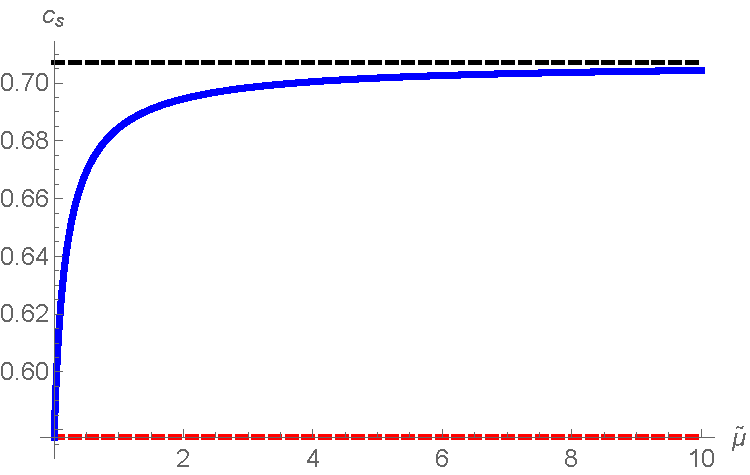
\includegraphics[width=3in]{Chapter_3_Folder_1806.06976/figures/soundspeed.pdf}
\end{center}
%\includegraphics[width=0.55\textwidth]{Dispersion_Relations}
%\includegraphics[width=0.45\textwidth]{Critical_velocity}
    \caption[This figure shows the value of the speed of sound as a function of the dimensionless parameter $\tilde{\mu}= \pi \left|\frac{\mu_B}{g_4 k} \right|$ for the massless theory.]{ The solid blue curve shows the slope of the phonon dispersion relation at $\p =0$ as a function of $\tilde\mu = \pi|\mu_B/g_4 k|$ for the massless theory, It interpolates between $c_s=1/\sqrt{3}$ at small $\tilde\mu$ and the conformal value of $c_s = 1/\sqrt{2}$ when $g_4$ is taken to zero.
%The left graph shows the dependence of the roton minimum on the coupling \textit{gk}. While the right graph shows the tangent at the minimum, whose slope is related to Landau's critical velocity ($ c_{L} $ ) associated with superfluid transitions.
}
\end{figure}
For non-zero scalar masses the phonon velocity is a nontrivial function of both $m$ and $\mu_B$.  For instance, at large values of $k$ and all other parameters held fixed, we obtain
%\begin{eqnarray}
%G&=&\frac{1}{\sqrt{\xi}}(\partial_{\mu}a^{\mu}-\xi \mathcal{F}_{i}\chi_{i})\nonumber\\
%\chi_{i}&=&(\varphi_{1}, \varphi_{2}, \varphi_{4}),~ \mathcal{F}^{a}_{i}=\frac{v}{2}\left(
%\begin{matrix}
%0~ \ 1~\ 0 \\ 1~ \ 0~\ 0 \\ \  0~0-1
%\end{matrix}
%right),
%\end{eqnarray}
%which adds the following gauge fixing term,
%\begin{eqnarray}
%S_{GF}=-\frac{1}{2}\int d^{3}x~ Tr (G^{a}G^{a})
%\end{eqnarray}
% One of these physical channels shows the existence of the so called \textit{phonon} as well as the \textit{roton} like excitations in the spectrum \cite{•}. The phonons are essentially the \textit{gapless} excitations (the so called Goldstone modes) that propagate with the velocity\footnote{The phonon velocity is obtained in the semi-classical (large $ k $) approximation. },
\bea
&&c^2_{s} \,=\,\frac{\mu_{B} ^2-m^2}{3\mu_{B} ^2-m^2}\,+\,\frac{\pi  \left(5 \mu_{B} ^2+m^2\right) (m^2 - \mu^2_B)^2 }{2 |k \mu_{B}| g_{4}   (m^2 -\mu^2_B)^2 }+ {O}(1/k^2)\,.
%\frac{\pi ^2  (m^2 -\mu^2_B)^2 \left(6m^4 -7m^2 \mu^2_B +31 \mu_{B}^4 \right)}{4 g_{4}^2 k^2(m^2 - 3\mu_{B}^2)^3}\nonumber\\
%&&+\frac{\pi ^3 \left(m^2-\mu_{B} ^2\right)^2 \left(893 \mu_{B} ^8+5 m^8-8 \mu_{B} ^2
%	m^6+318 \mu_{B} ^4 m^4-632 \mu_{B} ^6 m^2\right)}{8 g^3 k^3 \mu_{B}  \left(m^2-3 \mu_{B}^2\right)^4}+\mathcal{O}(1/k^{4})
\eea
The expression can be rewritten as a function of the two dimensionless parameters $\tilde \mu\,=\,\pi \mu_B/g_4 |k|$ and 
$\tilde m\equiv \pi m/g_4 |k|$.
%which is precisely given by the slope of the dispersion curve for small frequency ($ \omega $) and momenta ($ p_{x} $) and is gauge invariant.
%The part of the spectrum that contains rotons is characterized by a local minima at some finite momentum ($ p_{x} $). However, it could be checked quite easily that the dispersion relation possesses rotational invariance in the $ p_{x}-p_{y} $ plane which is an artefact of the rotational invariance (\ref{e17}) of the ground state mentioned previously.  
\paragraph{Level crossing:} The perturbative spectrum in the regime of small $\omega$ and $\p$ displays an interesting feature. This is a nontrivial consequence of crossing of energy levels which occurs as we tune the Chern-Simons level from $k=\infty$ to finite (large) values. This unavoidable crossing is between the phonon ($\omega_{\rm I (-)}$  branch) and the light state with energy $\omega_{\rm II(-)}$ which happens to be gapless with quadratic dispersion relation at $k=\infty$, but acquires a small gap $\sim 4\pi v^2/k$ at large $k$.  The crossing is accompanied by off-diagonal mixings between these two fluctuations. In the low energy, long wavelength limit $\omega, |\p| \ll \mu_B$ (where we are ignoring  $m$ for simplicity) it should suffice to focus attention on the two-level system comprising of the two lightest excitations. In this limit, the gapped modes only yield an overall multiplicative constant in the fluctuation determinant which takes the approximate form,
\be
\left(\omega^2 - c_s^2 \p^2\right)\left(\omega^2-\frac{\p^4}{4\mu^2}\,-\,\delta\right)\,-\,\varepsilon\, \p^4\,=0\,.\label{mixing}
\ee
The mixing term $\varepsilon\sim k^{-1}$, whilst  the gap generated for the branch $\omega_{\rm II(-)}$ with quadratic dispersion scales as  $\delta\sim k^{-2}$,  both  vanishing in the large $k$ limit.  The mixing must necessarily be momentum dependent so that the gapless phonon mode persists as a Goldstone boson for the broken $U(1)_B$. At low momentum the leading such contribution scales as $\p^4$ (using eq.\eqref{ci}). 
\begin{figure}[h]
\begin{center}
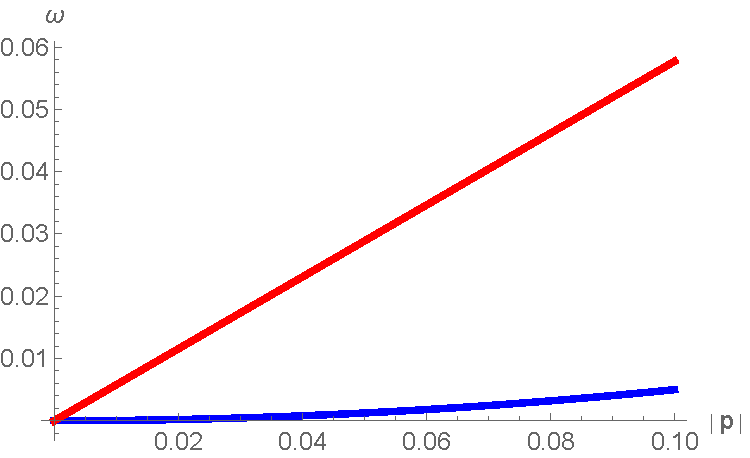
\includegraphics[width=2.3in]{Chapter_3_Folder_1806.06976/figures/crossing0.pdf}\hspace{0.8in}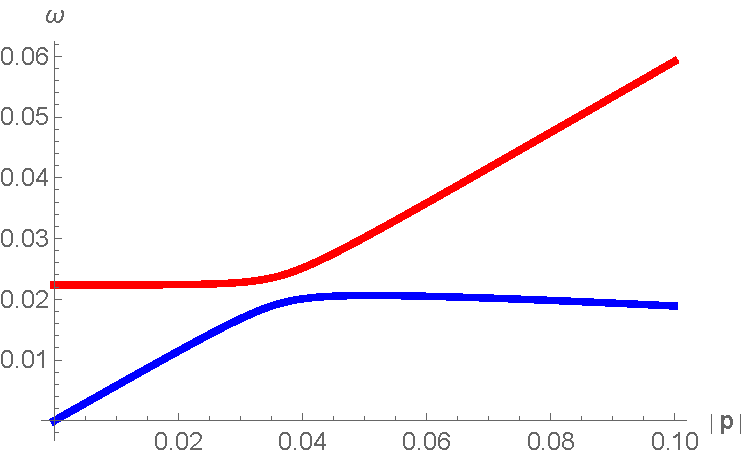
\includegraphics[width=2.3in]{Chapter_3_Folder_1806.06976/figures/crossing.pdf}
\end{center}
%\includegraphics[width=0.55\textwidth]{Dispersion_Relations}
%\includegraphics[width=0.45\textwidth]{Critical_velocity}
    \caption[This figure shows how the inclusion of a Chern-Simons term causes a level-splitting.]{ {\bf Left:} The $k=\infty$ theory displays two gapless excitations with linear and quadratic dispersion relation. {\bf Right:} At finite large $k$, the two modes potentially cross, and also mix. The diagonalized modes display  a splitting and ``repulsion" resulting in a local maximum in the phonon branch.
%The left graph shows the dependence of the roton minimum on the coupling \textit{gk}. While the right graph shows the tangent at the minimum, whose slope is related to Landau's critical velocity ($ c_{L} $ ) associated with superfluid transitions.
}\label{cross}
\end{figure}
The new solutions to \eqref{mixing} provide a qualitative description of the perturbed light spectrum at large, finite $k$.  
In particular, as shown in figure \ref{cross}, the two branches do not cross and the phonon branch displays a ``maxon" or a local maximum in its dispersion relation.  
For non-zero $\varepsilon$ the two dispersion relations (viewed as functions of $\p^2$) have a branch-point in the complex plane. For small enough $\varepsilon$, the location of the maximum in $\omega_{\rm I(-)}$ is close to the putative interesection point of the two curves.
The presence of this local maximum implies the existence of a ``roton" minimum since all dispersion curves must eventually increase linearly at large $|\p|$ consistent with UV relativistic invariance. 

\subsection{Roton minimum and complete spectrum}
Our main observation is that for any (large) finite value of $k$, consistent with being in the semiclassical regime the phonon branch always displays a roton minimum. 
At large $k$ and fixed $g_4$, the position of the maximum can be estimated quite easily. It sits close to the potential intersection point of the dispersion curves for $\omega_{\rm II(-)}$ and $\omega_{\rm I (-)}$. In the large $k$ regime, the former is flat, $\omega_{\rm II(-)}\,\approx\, 4\pi v^2/|k|$, while the latter is linear, $\omega_{\rm I(-)} \,\approx\, |\p|/\sqrt{3}$, and their putative intersection is at 
\be
k\gg 1,\,g_4\,{\rm fixed}: \qquad \left(\rm \omega_{\rm max},\, |\p|_{\rm max}\right)\,\approx\,\left(\frac{4\pi v^2}{|k|}, \, \frac{4\pi v^2\sqrt{3}}{|k|}\right)\,.
\ee
\begin{figure}[h]
\begin{center}
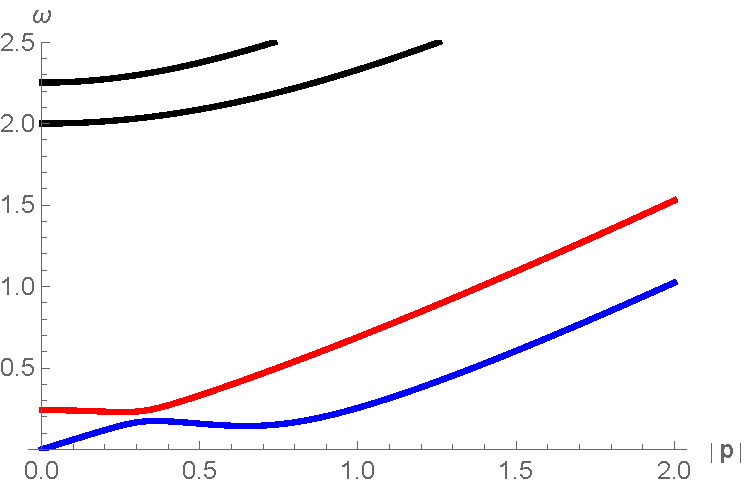
\includegraphics[width=2.8in]{Chapter_3_Folder_1806.06976/figures/spectrumk20.pdf}\hspace{0.1in}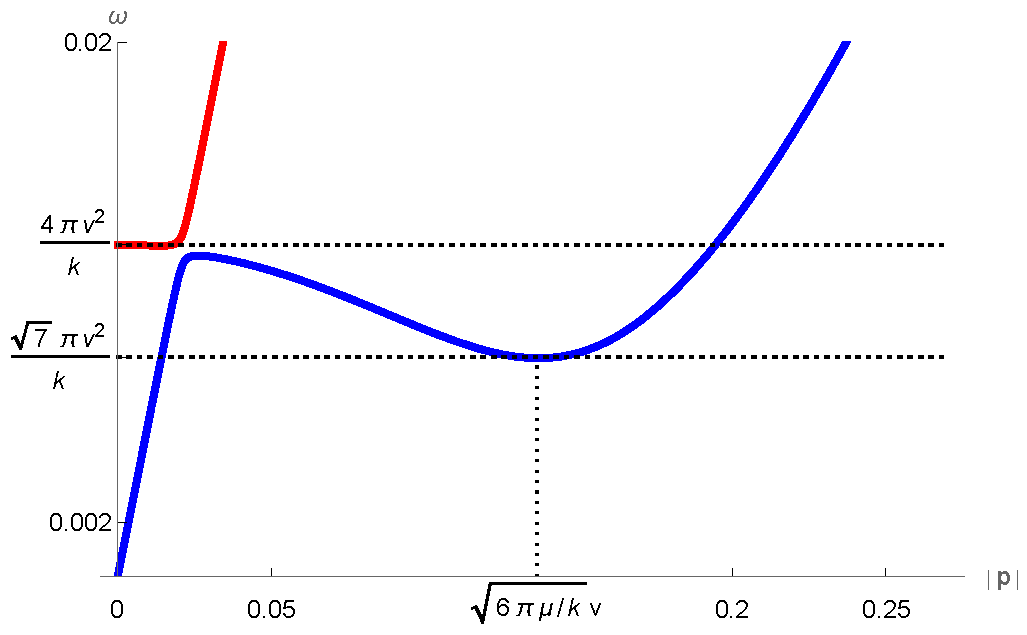
\includegraphics[width=2.8in]{Chapter_3_Folder_1806.06976/figures/rotonk500.pdf}
\end{center}
%\includegraphics[width=0.55\textwidth]{Dispersion_Relations}
%\includegraphics[width=0.45\textwidth]{Critical_velocity}
    \caption[This figure shows the position and heigh of the roton maximum, in addition to the mass of the lowest state for large values of $k$.]{ \small{{\bf Left:} The spectrum for $m=0$ with $\tilde\mu =\pi \mu_{B}/g_4 k =\pi/20 $. {\bf Right:} The two lightest states, including the phonon-roton branch (blue) with $\tilde\mu=\pi/500$. The dotted lines indicate the large-$k$ limiting values of the roton maximum and minimum.
}}
\label{largek}
\end{figure}
On the other hand, the location of the roton minimum is more subtle. In the large $k$ theory we expect the minimum to be located at parametrically small values close to the origin.  In fact, it turns out that $\omega_{\rm rot} \sim k^{-1}$ whilst  $\p_{\rm rot} \sim k^{-1/2}$. This can be checked by first performing the scaling 
\be
\omega\,=\,\frac{1}{k}\, \varpi\qquad\qquad \p\,=\, \frac{1}{\sqrt k}\,\varrho\,,
\ee
then substituting into the fluctuation determinant \eqref{ci}, and  the expression for $\omega'(\p)$  by differentiating \eqref{ci}. Subsequently, setting the determinant and $\omega'(\p)$ to zero, and then taking the large $k$ limit, we find (setting $m=0$ for simplicity):
\bea
&&3 \varrho^4\,-\,24 \pi  \mu_B  \varrho^2 v^2\,+\,4 \mu_B^2 \left(16 \pi ^2 v^4-\varpi ^2\right)\,=\,0\\\nonumber\\\nonumber
&&\varrho^4\,-\,12 \pi  \mu_B  \varrho^2 v^2\,+\,4 \mu_B^2 \left(16 \pi ^2 v^4-\varpi ^2\right)\,=\,0\,.
\eea
The solutions to these yield the roton minimum at large $k$ for the massless theory:
\be
k\gg 1: \qquad \left(\omega_{\rm rot},\,|\p|_{\rm rot}\right)\,=\,\left(\frac{\sqrt 7 \pi v^2}{k},\,\sqrt{\frac{6\pi \mu}{k}} \,v\right)\,,
\ee
where the VEV is given by \eqref{VEV} with $m=0$. The results for the roton minimum and maximum
agree perfectly with the numerical curves for the phonon-roton branch at large $k$, displayed in figure \ref{largek}. The qualitative nature of the dispersion relations persists for all values of $m$, $\mu_B$ and $g_4 k$. Figure \ref{spectmassive} shows the relevant plots for one non-zero value of $m$.
\begin{figure}[h]
\begin{center}
\includegraphics[width=2.3in]{Chapter_3_Folder_1806.06976/figures/spectrummassive.pdf}\hspace{0.3in}\includegraphics[height=2.3in]{Chapter_3_Folder_1806.06976/figures/spectrumcrit.pdf}
\end{center}
%\includegraphics[width=0.55\textwidth]{Dispersion_Relations}
%\includegraphics[width=0.45\textwidth]{Critical_velocity}
    \caption[This figure shows two plots. One depicts the spectrum in the massive case, whereas the other shows the free scalar theory coupled to Chern-Simons.]{ \small{{\bf Left}: The physical spectrum for the massive case. {\bf Right:} In the scale invariant situation, the dispersion relations have a universal form, independent of $k$ and $\mu$. The dotted blue line with slope $1/\sqrt 2$ matches the phonon velocity at low momentum.
}}
\label{spectmassive}
\end{figure}
\paragraph{Critical case with $g_4=m=0$:} A nontrivial aspect of the Bose condensed ground state is that all generic features of the spectrum of fluctuations persist even when $g_4=m=0$ (and $\mu_B\neq 0$) so that the classical theory is scale invariant.  The determinant of physical fluctuations \eqref{ci} simplifies greatly, and the relevant dispersion relations are obtained from its zeroes:
\bea
&&\tilde p\,\equiv\,\frac{|\p|}{\mu_B}\,\qquad \tilde \omega\,\equiv\,\frac{\omega}{\mu_B}\,,
\label{critdisp}\\\nonumber\\\nonumber
&& \tilde p^8\,-\,\tilde p^6 \left(4\tilde\omega ^2\,+\,\tfrac{28}{9}\right)\,+\,\tilde p^4 \left(  6\tilde \omega^4\,-\,\tfrac{4}{3}\tilde \omega ^2\,+\,\tfrac{160}{81}\right)\,-\, \tilde p^2 \left(4\tilde\omega ^6\,-\,12 \tilde \omega ^4+\tfrac{992}{81}\tilde\omega ^2-\tfrac{512}{81}\right)\\\nonumber\\\nonumber&&+\,\tilde \omega ^8\,-\,\tfrac{68 }{9}\tilde\omega ^6\,+\,\tfrac{1408 }{81}\tilde\omega ^4\,-\,\tfrac{1024 }{81}\tilde\omega ^2\,=\,0\,.
\eea
At zero momentum the energies of the four physical states are:
\be
\omega_{\rm I (-)}=0\,,\qquad\omega_{\rm I (+)}\,=\,\frac{4\mu_B}{3}\,,\qquad\omega_{\rm II (-)}\,=\,\frac{4\mu_B}{3}\,,\qquad \omega_{\rm II (+)}\,=\,2\mu_B\,,
\ee
so that two of the massive states become degenerate, 
whilst the roton maximum and minimum are at
\be
\left(\omega_{\rm max},\,|\p|_{\rm max}\right)\,=\,\left(0.553\mu_B,\,0.937\mu_B\right)\,,\qquad\left(\omega_{\rm rot},\,|\p|_{\rm rot}\right)\,=\,\left( 0.426\mu_B,\,1.487 \mu_B\right)\nonumber
\ee
We expect these results to be stable against quantum corrections for large enough $k$, since $\frac{1}{k}$ is the only small parameter in the system. It is interesting and somewhat unexpected (given that the roton minimum is often attributed to the presence of  a new scale)  that the roton persists in the theory where the chemical potential is the only dimensionful scale. 
\subsection{Landau critical velocity}
According to Landau's criterion, for a nonrelativistic superfluid flowing with velocity $v_s$ (with respect to a vessel or capillary), when the velocity exceeds a critical value \cite{Schmitt:2014eka} given by 
\be
v_{\rm crit} \,=\, {\rm min}_{|\bf p|} \left(\frac{\omega(\p)}{|\p|}\right)\,\implies \frac{\partial \omega}{\partial |\p|}\,=\,\frac{\omega}{|\p|}\,,
\ee
the fluid loses energy through dissipation and the superfluid phase can be wholly or partially destroyed e.g. by a condensate of rotons \cite{pitaevskii84, voskresenskii93}. In particular, \cite{pitaevskii84} argues for the appearance, within superfluid ${}^4{\rm He}$ flows, of a one dimensional periodic structure at rest with  respect to the walls so that the superfluidity criterion is not violated. The Landau criterion is derived by boosting the Bose condensate in the ground state along a particular direction (say the $+x$-axis) with a velocity $v_s$, and considering excitations that could reduce or dissipate the energy of the moving condensate. In the frame where the condensate has velocity $v_s$, the energy of a backscattered nonrelativistic excitation with momentum $\p$, causing dissipation  from the condensate, must  satisfy
\be
\omega(|\p|)\,-\,v_s|\p| <0,
\ee
where the second term is the result of  transformation under  the Galilean boost.
The critical value of the superfluid velocity is then given as $v_{\rm crit}\,=\,{\rm min}(\omega/|\p|)$. The arguments can also be carried out in the appropriate relativistic context (e.g.\cite{voskresenskii93, Schmitt:2014eka}). The critical velocity is inferred from the slope of the straight line passing through the origin and tangent to the dispersion curve for the phonon-roton branch (see dashed black line in figure \ref{spectmassive}).

 The behaviour of the critical velocity as a function of $\mu_B/g_4 k$ in the massless theory is shown in figure \ref{vcrit}.
 \begin{figure}[h]
\begin{center}
\includegraphics[height=2.0in]{Chapter_3_Folder_1806.06976/figures/vcrit.pdf}
\end{center}
%\includegraphics[width=0.55\textwidth]{Dispersion_Relations}
%\includegraphics[width=0.45\textwidth]{Critical_velocity}
     \caption[This figure shows the Landau critical velocity as a function of the dimensionless parameter $\pi\frac{\mu_B}{g_4 k}$ in the theory with $m=0$.]{ \small{The Landau critical velocity as a function of the dimensionless parameter $\pi\mu_B/g_4 k$ in the theory with $m=0$.}}
\label{vcrit}
\end{figure}
 At large $k$, the critical velocity vanishes as $1/\sqrt{k}$, and approaches a constant value, $v_{\rm crit}\approx 0.27$, in the theory with $g_4=0$.
 \subsection{The $U(2)_k$ theory}
 It is interesting to note the qualitative difference between $SU(2)$ and $U(2)$ gauge groups. In the latter case the $U(1)_B$ symmetry is gauged and the chemical potential is synonymous with a fixed background expectation value for the temporal component of the abelian gauge field.   The classical vacuum equations are satisfied by the same configuration as in the $SU(2)$ theory. The condensates of the scalar and gauge fields break both the $SU(2)$ and $U(1)_B$ local symmetries to a diagonal $U(1)$. 
 Since all symmetries are local we expect only massive physical states.   We obtain the physical fluctuations by employing Coulomb gauge for the abelian gauge field, and retaining the covariant $R_\xi$ gauge-fixing for the $SU(2)$ part. The situation with $m=g_4=0$ suffices to demonstrate the existence of the gap. In this case, the dispersion relations of the four physical states can be obtained from the roots of the following polynomial in  $(\tilde\omega,\,\tilde p)\,=\,\left(\omega/\mu_B, \,|\p|/\mu_B\right)$:
 \bea
 &&\tilde p\,\equiv\,\frac{|\p|}{\mu_B}\,\qquad \tilde \omega\,\equiv\,\frac{\omega}{\mu_B}\,,\\\nonumber\\\nonumber
&& \tilde p^8\,-\,\tilde p^6 \left(4\tilde\omega ^2\,+\,\tfrac{224}{81}\right)\,+\,\tilde p^4 \left(  6\tilde \omega^4\,-\,\tfrac{64}{27}\tilde \omega ^2\,+\,\tfrac{512}{243}\right)\,-\, \tilde p^2 \left(4\tilde\omega ^6\,-\,\tfrac{352}{27} \tilde \omega ^4+\tfrac{3328}{243}\tilde\omega ^2-\tfrac{4096}{729}\right)\\\nonumber\\\nonumber&&+\,\tilde \omega ^8\,-\,\tfrac{640 }{81}\tilde\omega ^6\,+\,\tfrac{4544 }{243}\tilde\omega ^4\,-\,\tfrac{10240 }{729}\tilde\omega ^2\,+\,\tfrac{16384}{59049}.
 \eea
 Unlike the $SU(2)$ theory \eqref{critdisp} we see that $\tilde\omega\,=\,\tilde p \,=\,0\ $ is no longer a solution. All states are gapped at $\p =0$, with the energies given by $\tilde \omega^2 = 16/9, 16/9, (22\pm5\sqrt{19})8/81$. The dispersion relations for non-zero $\p$ are shown in figure \ref{u2}.
  \begin{figure}[h]
\begin{center}
\includegraphics[height=2.0in]{Chapter_3_Folder_1806.06976/figures/u2.pdf}
\end{center}
%\includegraphics[width=0.55\textwidth]{Dispersion_Relations}
%\includegraphics[width=0.45\textwidth]{Critical_velocity}
      \caption[This figure shows the semiclassical spectrum of the $U(2)\simeq SU(2)\times U(1)$ theory.]{ \small{The semiclassical spectrum of the $U(2)\simeq SU(2)\times U(1)$ theory. All states are gapped. Nevertheless, the lightest state displays a roton-like minimum. The dotted blue line passing through the origin with slope $1/\sqrt 2$ is shown to emphasize the absence of  phonon-like linear dispersion.}}
\label{u2}
\end{figure}

 
 \section{The $SU(N>2)$ case}
 \label{sec4}
 We now generalize the above analysis for Chern-Simons scalar theory with $SU(N) $ gauge group. 
 We use lower case subscripts and superscripts, $(p,q,r\ldots)$ to label  fundamental and  antifundamental representation indices. The gauge covariant derivative is defined to include the chemical potential as a timelike background gauge field:
  \begin{eqnarray}
(D_{\mu})_{p}^{\ q}\,=\,\delta_{p}^{\ q}\,\partial_{\mu}\,+\,(A_{\mu})_{p}^{\ q}\,+\,i\mu_{B}\, \delta_{p}^{\ q}\,\delta_{\mu}^{0}\,. 
\end{eqnarray}
For general $N$, it is useful to define the quartic coupling so that a consistent large $N$ limit can be taken if necessary.  The potential contributions involving both gauge and scalar fields can be put together so that,
\begin{eqnarray}
V_{\rm CS}\,+\, V_{\rm scalar}&&=\, -\,\frac{k}{4\pi}\,\frac{2}{3}\,{\rm Tr}\left(A_\mu A_\nu A_\rho\right)\epsilon^{\mu\nu\rho}\,-\,
\Phi^{\dagger}\left(A^\mu + i\mu_B\eta^{\mu 0}\right)\left(A_\mu + i\mu_B\delta_{\mu}^0\right)\Phi\,\nonumber\\\label{sunpot}\\\nonumber
&&%-\,2\mu_{B}\Phi^{b\dagger}(A_0)_{b}\ ^{a}\Phi_{a}+(m^{2}-\mu_{B}^{2})\Phi_{a}^{\dagger}
+\,m^{2}\Phi^{\dagger}
\Phi\,+\,\frac{g_{4}}{N}(\Phi^{\dagger}\Phi)^{2}\,.
\end{eqnarray}
Assuming that the scalar obtains a vacuum expectation value, we can always use $SU(N)$ gauge rotations to place the VEV in the $N$-th component,
\begin{eqnarray}
\langle\Phi_{p}\rangle\,=\,\sqrt{N}\,v \,\delta_{p,N}\label{sclarvev}\,.
\end{eqnarray}
We have scaled out a factor of $\sqrt N$ in anticipation of the expected scaling in the  large-$N$ limit of vector models. In particular, the action for the matter fields should be ${\cal O}(N)$ in the large-$N$ limit.
The choice of scalar VEV leaves a residual $SU(N-1)$ gauge symmetry, which is then completely broken by the gauge field backgrounds in the ground state. In order to obtain the correct matrix equations of motion, we vary the action \eqref{sunpot} subject to a tracelessness condition for $SU(N)$ gauge fields, implemented by Lagrange multipliers $\Lambda^{0,1,2}$:
%The form of the VEV \eqref{sclarvev} makes it convenient to  identify the non-vanishing gauge field components using  the scalar potential eq.\eqref{sunpot} which becomes,
%\begin{eqnarray}
%V_{\rm CS}\,+\,V_{\rm scalar}&&=\,N\left[-\frac{k}{6\pi N}\,{\rm Tr}\left(A_\mu A_\nu A_\rho\right)\epsilon^{\mu\nu\rho}\,-\,
%v^{2}(A_{\mu})_{2}^{p}(A^{\mu})_{p}^{2}\,+\,2i\mu_{B}v^{2}(A_0)_{2}^{2}\,+\right.\nonumber\\\\\nonumber
%&&\left. +\,(m^{2}-\mu_{B}^{2})v^{2}\,+\,\frac{g_{4}}{2}v^{4}\right].
%\end{eqnarray}
%Next, we note down the CS potential which for the present case turns out to be,
%\begin{eqnarray}
%V_{CS}=\frac{ik}{2 \pi}
%(A_{0})_{a}\ ^{b}(F_{xy})_{b}\ ^{a}
%\end{eqnarray}
%where, $ (F_{ij})_{m}\ ^{n}=[A_{i},A_{j}]_{m}\ ^{n} $.
%Collecting all the non derivative terms together, the corresponding potential energy turns out to be,
%\begin{eqnarray}
%V=V_{CS}+V_{scalar}+\lambda \sum_{a=1}^{N}(A_{0})_{a}\ ^{a}
%\end{eqnarray} 
%where, $ \lambda $ the Lagrange multiplier. It is indeed quite trivial to note that the equation of motion corresponding to $ \lambda $ imposes the following tracelessnes condition,
%\begin{eqnarray}
%\sum_{a=1}^{N}(A_{0})_{a}\ ^{a}=(A_{0})_{1}\ ^{1}+(A_{0})_{N}\ ^{N}=0.
%\end{eqnarray}
%The variation of  the potential to obtain the equations of motion must respect the tracelessness of 
%$SU(N)$ matrices which is implemented naturally by a Lagrange multiplier constraint,
\be
V_{\rm CS}\,+\,V_{\rm scalar}\,\to\,V_{\rm CS}\,+\,V_{\rm scalar}\,+\,\Lambda^\mu {\rm Tr} (A_\mu)\,.
\ee
\subsection{Vacuum configuration}
The complete vacuum equations extremizing the potential function are:
\bea
&&-\frac{k}{4\pi}\, [A_\mu,A_\nu]\epsilon^{\mu\nu\lambda}\,-\,\left\{\Phi\Phi^\dagger,\,
\left(A^\lambda\,+\,i\mu_B\,\eta^{\lambda 0}{\bf 1}\right)\right\}\,+\,\Lambda^\lambda\,{\bf 1}\,=\,0\,,\qquad {\rm Tr} A_\mu\,=\,0\,,\nonumber\\\\\nonumber
&& -\,
(A_{\mu})_{N}^{p}(A^{\mu})_{p}^{N}\,+\,2i\mu_{B}(A_0)_{N}^{N}\,+\,(m^{2}-\mu_{B}^{2})\,+\,2g_{4}v^2\,=\,0\,.
\eea
The matrix $\Phi\Phi^\dagger$ is a projector, and given that the scalar VEV can be rotated into the lowest component, it has only one non-zero element,
\be
(\Phi\Phi^\dagger)_p^{\ q}\,=\,N\,\delta_{p,N}\,\delta^{q,N}\,v^2\,.
\ee
The Lagrange multipliers $\{\Lambda^\lambda\}$ are determined by taking the trace of each of the respective equations of motion so that, 
\be
\Lambda^\lambda\,=\,2v^2 \left[\left(A^\lambda\right)_N^{\ N}\,+\,i\mu_B\,\eta^{\lambda 0} \right]\,.
\ee
Following the hint provided by the $SU(2)$ vacuum solution, we take $A_0$ to be diagonal (note that  residual $SU(N-1)$ rotations can be used to diagonalize an $(N-1)\times (N-1)$ block of $A_0$). It then follows that the commutator $[A_x, A_y]$ must be diagonal $\sim {\rm diag}(1,1,\ldots, 1-N)$.  
This is reminiscent of the $N$-dimensional  representation of the $SU(2)$ algebra, where the off-diagonal ladder operators commute to yield a diagonal matrix. Motivated by this similarity, we find a simple solution for the Chern-Simons equations of motion:
\bea
&&\langle A_x\rangle_1^{\ q}\,=\, i\alpha\, \delta^{q,2}\,,\qquad \langle A_x\rangle_N^{\ q}\,=\,i\alpha\sqrt{N-1}\, \delta^{q,N-1}\\\nonumber\\\nonumber
&&\langle A_y\rangle_1^{\ q}\,=\, \alpha\, \delta^{q,2}\,,\qquad \langle A_y\rangle_N^{\ q}\,=\, -\alpha\sqrt{N-1}\, \delta^{q,N-1}\\\nonumber\\\nonumber
&&\langle A_x\rangle_p^{\ q}\,=\,i\alpha \left(\sqrt p\,\delta^{q, p+1}\,+\,\sqrt{p-1}\,\delta^{q,p-1}\right)\,,\qquad p\,=\,2,\ldots N-1\,\\\nonumber\\\nonumber
&&\langle A_y\rangle _p^{\ q}\,=\,\alpha \left(\sqrt p\,\delta^{q, p+1}\,-\,\sqrt{p-1}\,\delta^{q,p-1}\right)\,,\qquad p\,=\,2,\ldots N-1\,\\\nonumber\\\nonumber
&& \langle A_0\rangle_p^{\ q}\,=\, i\beta \left(\frac{1}{N}\delta_{p}^{\ q}\,-\,\delta_{p,N}\delta^{q,N}\right)\,, \qquad p,q\,=\,1\ldots N\,,
\eea
where the constants $\alpha$ and $\beta$ are determined by the VEV and chemical potential as,
\be
\alpha\,=\,\frac{\beta}{\sqrt N}\sqrt{\frac{\mu_B}{\beta}\,- \,\frac{N-1}{N}}\,,\qquad \beta\, =\, \frac{v^2}{\kappa}\,,\qquad \kappa\,\equiv\, \frac{k}{2\pi N}\,.\label{alphabeta}
\ee
The equation of motion for the scalar VEV (discarding the trivial extremum)  is then given by,
\be
-\frac{3}{\kappa^2}\left(1\,-\,\tfrac{1}{N}\right)^2\,v^4\,+\,v^2\left[2g_4\,+\,\frac{4\mu_B}{\kappa}\left(1-\tfrac{1}{N}\right)\right]\,-\,\left(\mu_B^2\,-\,m^2\right)\,=\,0\,.
\ee
Solving as a quadratic in $v^2$, only one solution is physical\footnote{The second root  yields $v^2 > \kappa\mu_B N/(N-1)$ which would render $\alpha$ imaginary. In addition, this solution does not have a smooth $k\to \infty$  limit.} and matches smoothly onto the semiclassical ($\kappa\gg 1$) limit:
\be
v^2\,=\,\tfrac{N\kappa}{3(N-1)}\left[\tfrac{g_4N\kappa}{(N-1)}\,+\,2\mu_B\,-\,\sqrt{\left(\tfrac{g_4N\kappa}{N-1}\,+\,2\mu_B\right)^2\,-\,3(\mu_B^2-m^2)}\right]\,.
\ee
This agrees precisely with the result \eqref{VEV}  for $N=2$ after we perform the rescalings, $v\to v/\sqrt{N}$ and $g_4 \to g_4 N$,  required to match the conventions adopted in our analysis of the $SU(2)$ theory. It is also worth remarking that the $N\to\infty$ limit, keeping $\kappa$ and $g_4$ fixed, can be readily taken and $v$  remains finite in this limit.

For the free massless scalar coupled to Chern-Simons fields ($m=g_4=0$), we obtain 
\be
v^2\,=\,\kappa \frac{N \mu_B}{3(N-1)}\,,\qquad \alpha\,=\,\frac{\mu_B}{3}\sqrt{\frac{2}{N-1}}\,.
\ee

\subsection{Interpretation as quantum Hall droplet state}
The vacuum configuration breaks the $SU(N)$ gauge symmetry completely. The scalar field VEV also breaks the global $U(1)_B$ spontaneously and therefore the spectrum must yield a massless phonon mode. As seen previously in the $SU(2)$ theory, the classical background is left invariant by a diagonal combination of $U(1)_B$, global colour and spatial rotations.  An $SO(2)$ rotation in the $x$-$y$ plane by an angle $\vartheta$, as in eq.\eqref{rotmatrix}, can be undone by a global gauge transformation generated by the diagonal matrix $J_3$:
\bea
&& U(1)_C: \quad \langle A_j\rangle\,\to e^{i\vartheta J_3}\,\langle A_j\rangle\, e^{-i\vartheta J_3}\\\nonumber\\\nonumber
&& J_3\,\equiv\,{\rm diag}\left(-\tfrac{N-1}{2}, -\tfrac{N-3}{2}, -\tfrac{N-5}{2}\ldots , \tfrac{N-3}{2}, \tfrac{N-1}{2}\right)\,.
\eea
$J_3$ is the $N$-dimensional representation of one of the three generators of the $SU(2)$ algebra.
The phase rotation of the scalar VEV generated by $J_3$ can clearly be compensated by a $U(1)_B$ transformation. 

An interesting feature of the vacuum solution is that the Hermitean matrices $i\langle A_x\rangle$ and $i\langle A_y\rangle$ provide a matrix realization of coordinates on the noncommutative plane:
\be
\left[i\langle A_x\rangle,\, i\langle A_y\rangle\right]\,=\,2i\alpha^2 \left[\begin{array} {c|c}\quad{\mathds{1}}_{(N-1)\times(N-1)}\quad\quad & 0 \\
& \\
\hline
0\,& 1-\, N \end{array}\right]\,
\ee
where the noncommutativity parameter is $2\alpha^2$ as defined in eq.\eqref{alphabeta}, and scales as $\alpha^2\sim 1/N$ for large $N$
\footnote{ It is tempting to look for solutions to the vacuum equations which are reducible and consist of irreducible lower dimensional blocks each satisfying the finite dimensional algebra  implied by the vacuum conditions.   We have not succeeded in finding any solutions of this type.}. Furthermore, it appears that the coordinates are restricted to within a disc or droplet: 
\be
\left(i\langle A_x\rangle\right)^2\,+\,\left(i\langle A_y\rangle\right)^2\,=\,2\alpha^2{\rm diag}\left(1\,,\,3\,,5\,,\ldots\,, (2N-3)\,,\, (N-1)\right)\,.\label{droplet}
\ee
The radius of the droplet is bounded in the large $N$ limit since $\alpha^2 \sim 1/N$ with limiting value
\be
R_{\rm droplet}\left.\right|_{N\to\infty}\,=\,2\beta\sqrt{\frac{\mu_B}{\beta}-1}\,.
\ee
The algebra of matrices is closely related to that of harmonic oscillator creation and annihilation operators, when written in terms of the ladder operators:
\be
A^\pm\,=\, i\left(\langle A_x\rangle \,\pm\, i\langle A_y\rangle\right)\,,
\ee
which, for any finite $N$, satisfy $(A^+)^N\,=\,(A^-)^N\,=\,0$.
Precisely the same set of matrices were introduced to describe the  fractional quantum Hall droplet in \cite{Polychronakos:2001mi}, building on the connection between Abelian noncommutative Chern-Simons theory on the plane and the quantum Hall fluid \cite{Susskind:2001fb}. The matrix model has also been shown to describe the low energy dynamics of vortices in 2+1 dimensional Yang-Mills-Higgs theory with a Chern-Simons term \cite{Tong:2003vy, Tong:2015xaa}.
In this picture, the matrices $i\langle A_x \rangle$ and $i\langle A_y\rangle $ parametrize the (noncommuting) coordinates of $N$ particles in the droplet.  As eq.\eqref{droplet} indicates, the particles are placed in concentric circles of radius $\sim \sqrt{2n-1}$ for $n=0,1,2,\ldots, N-1$. In the present context, the two matrices appear to deconstruct two dimensions (at large $N$) on top of the 2+1 spacetime dimensions in which the field theory is originally formulated. 

Given the finite density ``droplet" ground state for general $N$, we need to calculate the spectrum of fluctuations around it. This will be addressed in detail in future work  \cite{ongoing}. However, we can already make a few remarks.  The spectrum must exhibit a massless state corresponding to the phonon arising from the spontaneous breaking of $U(1)_B$. In the droplet picture,  physical excitations live only on the boundary of the quantum Hall droplet and are associated to area preserving deformations of the droplet boundary, subject to a Gauss' law constraint following from the Chern-Simons equations of motion \cite{Polychronakos:2001mi}.  These have a zero mode corresponding to rotations of the circular droplet ground state, which could naturally be identified with the phonon.  In the language of the $N\times N$ matrices comprising the gauge field fluctuations, in an appropriate gauge (more precisely, unitary gauge), the excitations are encoded in the entries of the $N$-th row and column of gauge field fluctuations of ${\cal A}_x$ and ${\cal A}_y$, all other fluctuations corresponding to pure gauge or ``bulk" degrees of freedom  of the droplet. 
It would be extremely interesting to flesh out this picture in detail and explore the implications of this interpretation for the spectrum of the theory for generic $N$, and in particular its large-$N$ limit.

\textcolor{red}{\section{Vortices in U(2) and SU(2) Chern-Simons scalar theories.}}
Before we conclude this chapter, we address the possibility of a vortex solution in the background of the ground state we have seen above (\ref{E14}, \ref{VEV}). If vortices exist in this model, we expect them to be quite different from the ones we encountered in Chapter 2, since here we are considering a non-abelian theory. 

Non-abelian vortices have been studied in a number of occasions in the past \cite{deVega:1986eu, Kumar:1986yz, Blazquez-Salcedo:2013roa, NavarroLerida:2009dm}. These are notably different to their abelian counterparts since the scalars appearing in those models, are in the adjoint representation. This allows for the VEV to remain invariant under the center of the gauge group. If $z\in Z(G)$, where $Z(G)$ is the center of $G$, then by definition $z$ commutes with all elements in the group. Thus, if an adjoint scalar $\Phi$ has a non-zero VEV, then under a gauge transformation generated by z, we have $\Phi \rightarrow z\Phi z^{\dag} =\Phi z z^{\dag} = \Phi$. In the above cases, the gauge group is $SU(N)$ with center $Z(SU(N)) =\mathbb{Z}_N$. This means that the action of the gauge group $SU(N)$ on the adjoint scalars reduces to an $SU(N)/Z(SU(N))= SU(N)/\mathbb{Z}_N$. This gives rise to the possibility of a topological vortex, since $\pi_1(SU(N)/\mathbb{Z}_N)=\mathbb{Z}_N$, even though $\pi_1(SU(N))$ is trivial.

In contrast to these studies, we will be interested in fundamental scalars so this argument does not apply directly to our subject matter. However, due to the appearance of a non-zero chemical potential, we have found out that non-zero VEVs in the gauge sector come to play a role. Since the gauge fields are in the adjoint representation, this allows for the same type of argument for topological stability to reappear in a theory with fundamental matter. In the context of Yang-Mills theory, this type of vortex has been explored by \textit{Gorbar, Jia \& Miransky} \cite{Gorbar:2005pi}.\\  
\indent Similarly to the situation that we encountered in Chapter \ref{ch:Chapter_2}, in the non-abelian case, we also observe a non-trivial ground state. This means that we can expect that there will be a circularly symmetric classical solution that interpolates between this ground state at infinity and the zero fields configuration at the centre. And just as we elaborated in the previous paragraph, we expect to have two different types of topological vortices, depending on whether we are interested in the U(2) or SU(2) system. First, we focus our attention on the $U(2)$ theory.

%\textcolor{red}{Miransky \textit{et al} non-zero chemical potential papers \cite{Gorbar:2005pi, Gusynin2004}}\\
%\textcolor{red}{Non-abelian vortices can also arise through a mechanism such as \cite{Vachaspati:1991cs}}\\
%\textcolor{red} Write up the holonomy


\section{U(2) theory}
In the $U(2)$ theory, we don't expect to find global vortices, since the global $U(1)$ symmetry in now gauged. In this model, we expect to find \textit{two types} of vortices. The first one will be associated to a winding in the $U(1)$ and as such it is classified by $\pi_1(U(1))= \mathbb{Z}$. This leads to a charged, hence non-equilibrium configuration, exactly as was the case in Chapter 2. For this reason, we need to introduce a background charge density in order to guarantee that the configuration is charge neutral. The second type of vortex owes its existence to the unusual form of the VEV, namely the fact that the adjoint vector boson acquires non-zero expectation values. This vortex will be classified by $$\pi_1(SU(2)/Z(SU(2)))= \pi_1(SU(2)/\mathbb{Z}_2) = \mathbb{Z}_2$$ The action for the $U(2)$ theory can be written down as follows.    
\begin{align}
    S^{\text{SU(2)}}_{\text{CS}} &= \frac{k}{4 \pi} \int d^3x \; \epsilon^{\mu \nu \rho} \; \mathrm{Tr} \left[A_{\mu} \partial_{\nu}A_{\rho}+ \frac{2}{3} A_{\mu} A_{\nu}A_{\rho} \right], \\
    S^{\text{U(1)}}_{\text{CS}} &= \frac{k'}{4 \pi} \int d^3x \; \epsilon^{\mu \nu \rho} B_{\mu} \partial_{\nu} B_{\rho},\\
    S_{\text{matter}}&= - \int d^3x \left[ \left(D_{\mu} \Phi \right)^{\dag} \left(D^{\mu} \Phi \right) + V\left(\Phi^{\dag}\Phi \right)\right], \\
    S &= S^{\text{SU(2)}}_{\text{CS}} + S^{\text{U(1)}}_{\text{CS}} + S_{\text{matter}}, \\
    D_{\mu} &= \partial_{\mu} + A_{\mu}+B_{\mu} +i \mu_B \delta_{\mu}^{\;\; 0},
\end{align}
where we have allowed for possibly different Chern-Simons levels for the abelian and non-abelian levels $k\neq k'$, consistent with the statements of duality that we saw in Chapter 1 (\ref{eq:Fermi-Bose_1}-\ref{eq:Fermi-Bose_3}). We are restricting the potential  here to be quartic $$V\left(\Phi^{\dag} \Phi \right)= m^2 \Phi^{\dag} \Phi + g_4\left( \Phi^{\dag} \Phi\right)^2$$and that the magnitude of the mass squared term is smaller than the magnitude of the chemical potential $m^2<\mu_B^2$ in order to guarantee symmetry breaking and the existence of the ground state we studied in the previous sections. A sixth order monomial can also be included in the potential without changing the physics qualitatively, hence we choose to omit it here for simplicity. This leads to the classical equations of motion for the gauge sector.
\begin{align}
    \frac{k}{2 \pi} F_{\mu \nu} = \epsilon_{\mu \nu \lambda} J^{\lambda}\\
    \frac{k'}{2\pi} f_{\mu \nu} = \epsilon_{\mu \nu \lambda} \frac{1}{2} \mathrm{Tr} \left[\hat{J}^{\lambda} \right],
\end{align}
where
\begin{align}
    F_{\mu \nu}&= \partial_{\mu} A_{\nu} - \partial_{\nu}A_{\mu} + [A_{\mu}, A_{\nu}], \qquad f_{\mu \nu} = \partial_{\mu} B_{\nu} - \partial_{\nu} B_{\mu}, \\
    \hat{J}^{\lambda} &= \sqrt{-g} g^{\lambda \nu} \left( \Phi \left( D_{\nu} \Phi\right)^{\dag} - D_{\nu} \Phi \Phi^{\dag}   -2i \mu_B \delta^{\;\; 0}_{\nu} \Phi \Phi^{\dag}  \right), \\
    J^{\lambda} &= \hat{J}^{\lambda} - \frac{1}{2}\mathrm{Tr}\left[\hat{J}^{\lambda} \right]\mathbb{I} \qquad \implies \qquad \mathrm{Tr}\left[J^{\lambda}\right]=0.
\end{align}
The scalar equations are 
\begin{align}
    \left(D_{\mu} + i\mu \delta_{\mu}^{\;\; 0} \right) \left[\sqrt{-g} \left(D^{\mu}+i \mu g^{\mu 0}\right)\right] \Phi = - \sqrt{-g} \frac{\delta V}{\delta \Phi^{\dag}}. \label{eq:U2_scalar_EOM}
\end{align}
Consider the ansatz
\begin{align}
    A_{\mu} &= i \left(a_{\mu}^3 \sigma_3 + a_{\mu}^+ \sigma_{+} +a_{\mu}^{-} \sigma_{-} \right), \label{eq:U2_ansatz_non_abelian_gauge} \\
    B_{\mu} &= i \left( a_{\mu} \mathbb{I} \right), \label{eq:U2_ansatz_abelian_gauge}\\
    \Phi &=  e^{i n \theta} \begin{pmatrix}
        0\\
        \varphi(r)\\
    \end{pmatrix}, \qquad n\in \mathbb{Z}, \qquad \varphi(r) \xrightarrow{r \rightarrow \infty} v, \label{eq:U2_ansatz_scalar}
\end{align}
    where the matrices
    \begin{align}
        \sigma_3 = \begin{bmatrix}
            1 & 0 \\
            0 & -1 \\
        \end{bmatrix}, \qquad \mathbb{I}= \begin{bmatrix}
            1 & 0\\
            0 & 1\\
        \end{bmatrix} \\
        \sigma_+ =\begin{bmatrix}
            0 & 1\\
            0 & 0\\
        \end{bmatrix}, \qquad \sigma_- = \begin{bmatrix}
            0 &0\\
            1 &0\\
        \end{bmatrix},
    \end{align}
    are a basis of $U(2)$ that allows us to think of $a_{\mu}^{+}$ as the complex conjugate of $a_{\mu}^{-}= (a_{\mu}^{+})^*$. Further, restricting to a static, circularly symmetric solution, the ansatz becomes
\begin{align}
    a_{0/\theta}^{+} &= \tilde{g}_{0/\theta}(r)e^{-i \theta + i\alpha}\quad, \qquad \qquad a_{0/\theta}^{-} = \tilde{g}_{0/\theta}(r)e^{+i \theta - i\alpha}, \label{eq:U2_gauge_ansatz_static_1}\\
    a_{r}^{+} &= \tilde{g}_{r}(r)e^{-i \theta + i\left(\alpha + \frac{\pi}{2} \right)}, \qquad \qquad a_{r}^{-} = \tilde{g}_{r}(r)e^{+i \theta - i\left(\alpha + \frac{\pi}{2} \right)}, \label{eq:U2_gauge_ansatz_static_2}\\
    a_{\mu}^{(3)}&= f_{\mu}(r),\qquad \qquad \qquad \qquad f_r(r)=0, \label{eq:U2_gauge_ansatz_static_3}\\
    a_{\mu}&= a_{\mu}(r),\qquad \qquad \qquad \qquad a_r(r)=0\label{eq:U2_gauge_ansatz_static_4},
\end{align}
where all of $\tilde{g}_{\mu} \in \mathbb{R}$. Note the $\frac{\pi}{2}$ shift of the phase of the $g_r$ component relative to the rest of the functions. This is analogous to how the vacuum components of $A_{\theta}$ and $A_r$ relate to one another. The phase factor $e^{i \alpha}$ has to do with the remaining global colour-flavour locked $U(1)$ symmetry in the system. Using the form of the ansatz above we have
    \begin{align}
        \Phi \Phi^{\dag} = \varphi(r)^2 \begin{pmatrix} 
            0 & 0\\
            0 & 1\\
        \end{pmatrix} = \varphi(r)^2 \sigma_- \sigma_+.
    \end{align}
    And using the following relations in order to simplify the equations of motion
    \begin{align}
        [\sigma_+, \sigma_-] = \sigma_3, \qquad [\sigma_3, \sigma_+] = 2 \sigma_+, \qquad [\sigma_3, \sigma_-] = -2 \sigma_-.
    \end{align}
    The system of differential equations then simplifies to
    \begin{align}
        \frac{k}{2 \pi } \left(f_{\theta}' - 2\tilde{g}_r \tilde{g}_{\theta}\right) &= -r \left(a_0 + \mu - f_0\right) \phi^2,\\
        \frac{k}{2 \pi} \left(\tilde{g}_{\theta}' + \tilde{g}_r - 2 \tilde{g}_r f_{\theta} \right) & = r\tilde{g}_0 \phi^2, \\
        \frac{k'}{2 \pi} a_{\theta}' &= r \left(a_0 +\mu - f_0 \right)\phi^2 - rJ_0, \\
        \frac{k}{2\pi} \left(f_0'+2 \tilde{g}_0\tilde{g}_r\right) &= \frac{1}{r} \left(a_{\theta}+n - f_{\theta}\right)\phi^2, \\
        \frac{k}{2\pi}\left(\tilde{g}_0' + 2 f_0 \tilde{g}_r \right) &=\frac{1}{r} \tilde{g}_{\theta}\phi^2, \\
        \frac{k'}{2\pi} a_0'&= \frac{1}{r} \left(a_{\theta}+n - f_{\theta}\right) \phi^2, \\
        \frac{k}{2\pi} \left(\tilde{g}_0 - 2\left(f_{\theta} \tilde{g}_0 - \tilde{g}_{\theta} f_0\right)\right) &= r \tilde{g}_r \phi^2,
    \end{align}
    where $J_0$ is determined by requiring that the system is neutral when evaluated at the VEV. This implies that
    \begin{align}
        J_0 = -\frac{\pi v^2}{k} \left(\frac{\mu k}{\pi}- v^2 \right).
    \end{align}
Inserting the ansatz (\ref{eq:U2_ansatz_non_abelian_gauge}-\ref{eq:U2_ansatz_scalar}) and (\ref{eq:U2_gauge_ansatz_static_1}-\ref{eq:U2_gauge_ansatz_static_4}) into the scalar equation of motion \ref{eq:U2_scalar_EOM} we arrive at
\begin{align}
    \frac{1}{r} \frac{d}{dr} \left(r \varphi\right)+ &\varphi \left( \left(f_0 -a_0 -\mu\right)^2 + |\tilde{g}_0|^2 - \left(a_r -f_r\right)^2 - |\tilde{g}_r|^2 \right)\nonumber \\
    &+ \varphi \left(-\frac{1}{r^2} \left(f_{\theta} - a_{\theta} -n\right)^2 +|\tilde{g}_{\theta}|^2 \right) = - \frac{\delta V}{\delta \Phi^{\dag}}.
\end{align}
We would like a solution that asymptotes to the ground state that we explored in Chapter \ref{ch:Chapter_3} (\ref{E14}, \ref{VEV}). This implies the following boundary conditions
\begin{align}
    \varphi &\xrightarrow{r \rightarrow \infty} v, \qquad \qquad \qquad & \varphi \xrightarrow{r \rightarrow 0} 0,\\
    \tilde{g}_{\theta} &\xrightarrow{r \rightarrow \infty} r \frac{\pi v}{k} \sqrt{ \frac{\mu k}{\pi} -v^2}, &f_{\theta} \xrightarrow{r \rightarrow \infty}0,\\ 
    \tilde{g}_0 &\xrightarrow{r \rightarrow \infty} 0, &f_0  \xrightarrow{r \rightarrow \infty}\frac{\pi v^2}{k},\\
     a_0 &\xrightarrow{r \rightarrow \infty} 0, &a_{\theta} \xrightarrow{r \rightarrow \infty} 0,\\
    & \qquad\qquad\qquad\qquad  \tilde{g}_r \xrightarrow{r \rightarrow \infty} \frac{\pi v}{k} \sqrt{ \frac{\mu k}{\pi} -v^2}.  & 
\end{align}




\section{SU(2) theory}

The $SU(2)$ equations of motion are determined by requiring that the trace of the $U(2)$ equations of motion vanishes. This leads to the simplified system
    \begin{align}
        \frac{k}{2 \pi} \left(\partial_{r} a_{\theta}^3 - \partial_{\theta} a_r^{(3)} + i \left(a_r^+ a_{\theta}^- - a_r^- a_{\theta}^{+} \right) \right) &= -r \left(\mu - a^{(3)} \right)\phi^2 \\
        \frac{k}{2 \pi} \left(\partial_r a_{\theta}^{+} - \partial_{\theta} a_r^{+} +2i \left(a_r^{(3)} a_{\theta}^{+} - a_r^{+} a_{\theta}^{(3)} \right) \right) &=r a_0^{+} \phi^2  \\
        \frac{k}{2 \pi}\left(\partial_{0}a_r^{(3)} - \partial_r a_0^{(3)} + i \left(a_0^+ a_r^- - a_0^- a_r^+  \right)  \right) &= \frac{1}{r} \left(n - a_{\theta}^{(3)} \right) \phi^2  \\
        \frac{k}{2 \pi} \left( \partial_0 a_r^+ - \partial_r a_0^+ + 2i \left( a_0^{(3)} a_r^+ -a_0^+ a_r^{(3)} \right) \right) &= -\frac{1}{r} a_{\theta}^+ \phi^2  \\
        \frac{k}{2 \pi} \left(\partial_{\theta} a_0^{(3)} - \partial_0 a_{\theta}^{(3)} + i \left(a_{\theta}^+ a_0^- - a_{\theta}^- a_0^{+} \right) \right) &= -r  a_r^{(3)} \phi^2 \\
        \frac{k}{2 \pi} \left(\partial_{\theta} a_0^+ - \partial_0 a_{\theta}^+ + 2i \left(a_{\theta}^{(3)} a_0^+ - a_{\theta}^+ a_0^{(3)} \right) \right) &=-r a_r^+ \phi^2.
    \end{align}




    \begin{align}
        \frac{k}{2 \pi } \left(f_{\theta}' - 2\tilde{g}_r \tilde{g}_{\theta}\right) &= -r \left(\mu - f_0\right) \phi^2\\
        \frac{k}{2 \pi} \left(\tilde{g}_{\theta}' + \tilde{g}_r - 2 \tilde{g}_r f_{\theta} \right) & = r\tilde{g}_0 \phi^2 \\
        \frac{k}{2\pi} \left(f_0'+2 \tilde{g}_0\tilde{g}_r\right) &= \frac{1}{r} \left(n - f_{\theta}\right)\phi^2 \\
        \frac{k}{2\pi}\left(\tilde{g}_0' + 2 f_0 \tilde{g}_r \right) &=\frac{1}{r} \tilde{g}_{\theta}\phi^2 \\
        \frac{k}{2\pi} \left(\tilde{g}_0 - 2\left(f_{\theta} \tilde{g}_0 - \tilde{g}_{\theta} f_0\right)\right) &= r \tilde{g}_r \phi^2.
    \end{align}


    \section{Discussion}
    We took the vacuum solutions in the SU(2) and U(2) theories found in Chapter \ref{ch:Chapter_3} and postulated the existence of vortex solutions asymptoting to these vacua. We found a consistent circularly symmetric ansatz and derived the equations of motion. Just as the ground state has an unbroken $U(1)$ symmetry, the solutions of the equations seem to also be parametrized by one real, compact parameter. Since the $SU(N)$ solutions correspond to a winding in the global symmetry, we expect that their energies will diverge in the infinite volume limit. However, in the $U(2)$ case the abelian symmetry is gauged so we expect the vortices in this model to be of finite energy. Further, due to the non-trivial vacuum structure, we expect these solutions to be topologically stable. We leave the numerical analysis of these solutions for further work.


\textcolor{red}{ends here}
\section{Summary and future directions}
\label{sec5}
There are several immediate questions of interest that follow on from the results above.
The Bose condensed vacuum should have semiclassical vortex solutions, and it would be interesting to understand their explicit construction given the non-Abelian nature of the vacuum configuration. The ground state has a $U(1)$ colour-flavour locked global symmetry. A vortex solution that breaks this global symmetry will have an internal zero mode corresponding to a $U(1)$ moduli space of solutions.  Such vortices in a (non-Abelian) Higgs phase with noncommuting VEVs, carrying internal zero modes have been encountered previously in different contexts \cite{Markov:2004mj, Auzzi:2008ep, Auzzi:2009es}. The physical properties of such vortices and their role in the Bose-Fermi duality would be extremely interesting to explore.

The  origin of roton-like minima is often attributed to long range interactions. The interpretation of the background VEVs as noncommuting ``coordinates" for a quantum Hall droplet could thus provide a natural route to establish the existence of roton-like excitations\footnote{See e.g. \cite{Castorina:2004yd} for a discussion of the relation between noncommutative field theory and roton excitations in bosonic and fermionic systems.} for general $N>2$.  In general, the computation of the spectrum of excitations and their dispersion relations about the Bose condensed ground state should be facilitated by the connection to the droplet picture of \cite{Polychronakos:2001mi}. The goal would be to eventually understand the putative matching between the  spectra of the bosonic theory at weak 't Hooft coupling ($\lambda_B\ll 1$) and that of the dual critical fermion theory (coupled to Chern-Simons) at strong 't Hooft coupling $(\lambda_F\to 1)$. Perhaps the most puzzling aspect of this is the interpretation of the Higgsed ground state. When $\lambda_F=0$, and a $U(1)_B$ chemical potential is switched on in the critical theory, we do not  expect fermion bilinears to condense (see e.g. \cite{Hands:1998he}). As $\lambda_F$ is increased from zero it is conceivable that the effective potential for charged fermion bilinears carrying $U(1)_B$ favours a condensate either for any non-zero $\lambda_F$ or at some critical value. It would be extremely interesting to understand the behaviour of the large-$N$ effective potential for fermion bilinears for non-zero $\lambda_F$ and $\mu_B$.



 A related question has recently been explored in \cite{Choudhury:2018iwf} where Bose-Fermi duality at finite temperature and in the presence of scalar condensate has been established in the large-$N$ 't Hooft limit. We will need to understand  the modification of the zero temperature finite density state, and in particular the background gauge fields VEVs, by any non-zero temperature since the  Euclidean finite temperature theory is effectively two dimensional at long distances and thus fluctuations in the  phase of the scalar VEV are unsuppressed.  It will be interesting to understand the fate of the phonon-roton mode at finite temperature and non-zero 't Hooft coupling in the Chern-Simons-scalar theory.


%\acknowledgments We would like to thank Justin David, Jeff Murugan and Carlos N\'u\~nez for  enjoyable discussions.
%SPK acknowledges support from STFC grant ST/L000369/1. SS is supported by an STFC studentship under the DTP grant ST/N504464/1. DR is supported by a Royal Society SERB-Newton Fellowship.
\newpage

%\appendix
%\section{Determinant of fluctuation matrix for $SU(2)$ }
%The determinant for the physical fluctuations is given in terms of frequency $\omega$ and momentum ${\bf p}$ as,
%\be
%\omega^8\,+\,\mu^2_BC_3\,\omega^6\,+\,\mu^4_BC_2 \,\omega^4 \,+\,\mu^6_BC_1\, \omega^2 \,+\,\mu^8_B\, C_0\,=\,0\,.
%\ee
%Assuming ${k>0, \mu_B>0}$ the coefficients $\{C_i\}$ are (for general choice of signs, it is understood that $k$ and $\mu_B$ will be replaced by their absolute values below):
%\bea
%&& C_0\,=\,\left(\frac{{\bf p}^2}{\mu_B^2}\right)^4\,+\,\left(\frac{{\bf p}^2}{\mu_B^2}\right)^3\left(\frac{m^2}{\mu_B^2}-1+\frac{6 g_4 v^2}{\mu_B^2}+\frac{17\pi^2 v^4}{k^2\mu_B^2}-\frac{12\pi v^2}{k\mu_B}\right)\,+\,\left(\frac{{\bf p}^2}{\mu_B^2}\right)^2\times\nonumber\\\nonumber\\\nonumber
%&&\times\left(\frac{16 \pi ^2  m^2 v^4}{k^2 \mu_B^4}-\frac{12 \pi m^2 v^2}{k \mu^3_B}+\frac{96 \pi ^2 g_4 v^6}{k^2 \mu_B^4}-\frac{72 \pi g_4 v^4}{k \mu_B^3}+\frac{16 \pi^4  v^8}{k^4 \mu_B^4}-\frac{12 \pi ^3  v^6}{k^3 \mu_B^3}-\frac{16 \pi ^2
%   v^4}{k^2 \mu^2_B}\right.\\\nonumber\\\nonumber
%   &&\left.+\frac{12 \pi  v^2}{k \mu_B}\right)\,+\,\left(\frac{{\bf p}^2}{\mu_B^2}\right)\left(-\frac{384 \pi ^3 g_4 v^8}{k^3 \mu_B^5}+\frac{384 \pi ^2 g_4 v^6}{k^2 \mu_B^4}+\frac{960 \pi ^5
%   v^{10}}{k^5 \mu_B^5}-\frac{1728 \pi ^4 v^8}{k^4 \mu_B^4}\right.\\\nonumber\\\label{ci}
%   &&\left.-\frac{64 \pi ^3  m^2 v^6}{k^3 \mu_B^5}+\frac{832 \pi ^3
%    v^6}{k^3 \mu_B^3}+\frac{64 \pi ^2 m^2 v^4}{k^2 \mu_B^4}-\frac{64 \pi ^2 v^4}{k^2 \mu_B^2}\right)\\\nonumber\\\nonumber
%&&  C_1\,=\, -4\left(\frac{{\bf p}^2}{\mu_B^2}\right)^3\,+\,\left(\frac{{\bf p}^2}{\mu_B^2}\right)^2\left(-5-\frac{3m^2}{\mu_B^2}-\frac{18g_4v^2}{\mu_B^2}-\frac{51\pi^2 v^4}{k^2\mu_B^2}+\frac{28\pi v^2}{k\mu_B}\right)\,+\\\nonumber\\\nonumber
%&&+\left(\frac{{\bf p}^2}{\mu_B^2}\right)\left(4 
%   -4 \frac{m^2}{\mu_B ^2}-24 \frac{g_4  v^2}{\mu_B ^2}-\frac{192 \pi ^2 g_4 v^6}{k^2\mu_B ^4}+\frac{72 \pi   g_4 v^4}{k\mu_B ^3}-\frac{32 \pi ^4
%  v^8}{k^4 \mu_B ^4}\right.\\\nonumber\\\nonumber
%  &&\left.+\frac{76 \pi ^3    v^6}{k^3\mu_B ^3}-
%  \frac{32 \pi ^2  m^2 v^4}{k^2\mu_B ^4}-\frac{84 \pi ^2
%    v^4}{k^2\mu_B ^2}+\frac{12 \pi  m^2 v^2}{k\mu_B ^3}-\frac{28 \pi  v^2}{k\mu_B }\right)\,-\frac{384 \pi ^2g_4 v^6}{k^2 \mu_B ^4}\\\nonumber\\\nonumber
%    &&-\frac{64 \pi ^4 v^8}{k^4 \mu_B ^4}+\frac{256 \pi ^3 v^6}{k^3 \mu_B
%   ^3}-\frac{64 \pi ^2  m^2 v^4}{k^2 \mu_B^4}-\frac{192 \pi ^2v^4}{k^2 \mu_B^2}\\\nonumber\\\nonumber
%   && C_2\,=\,6\left(\frac{{\bf p}^2}{\mu_B^2}\right)^2\,+\,\left(\frac{{\bf p}^2}{\mu_B^2}\right)\left(\frac{18  g_4 v^2}{\mu_B^2}+\frac{51 \pi ^2 v^4}{k^2 \mu_B^2}-\frac{20 \pi v^2}{k \mu_B }+\frac{3
%   m^2}{\mu_B ^2}+13\right) \,+\frac{96 \pi ^2g_4 v^6}{k^2 \mu_B^4}
%   \\\nonumber\\\nonumber
%   &&+\frac{24  g_4 v^2}{\mu_B^2}
%   +\frac{16 \pi ^4  v^8}{k^4 \mu_B^4}-\frac{64 \pi ^3 v^6}{k^3 \mu_B^3}+\frac{16 \pi ^2 m^2 v^4}{k^2 \mu_B^4}+\frac{116 \pi ^2 v^4}{k^2 \mu_B^2}-\frac{16 \pi  v^2}{k \mu_B }+\frac{4 m^2}{\mu_B^2}+12 \\\nonumber\\\nonumber
%   && C_3\,=\, -4\left(\frac{{\bf p}^2}{\mu_B^2}\right)-\frac{6 g_B v^2}{\mu_B^2}-\frac{17 \pi ^2  v^4}{k^2 \mu_B^2}+\frac{4 \pi v^2}{k \mu_B
%   }-\frac{m^2}{\mu_B^2}-7
%\eea
%
%

%
% this file is called up by thesis.tex
% content in this file will be fed into the main document
    \graphicspath{{Background_Folder/figures/PNG/}{Background_Folder/figures/PDF/}{Background_Folder/figures/}}

%: ———————-- introduction file header ———————--
\chapter{Vortices in U(2) and SU(2) Chern-Simons scalar theories.}

\label{ch:Chapter_4}



Non-abelian vortices have been studied in \cite{deVega:1986eu, Kumar:1986yz, Blazquez-Salcedo:2013roa, NavarroLerida:2009dm}. These are notably different to their abelian counterparts since the scalars appearing in those models, are in the adjoint representation. This allows for the VEV to remain invariant under the center of the gauge group. If $z\in Z(G)$, where $Z(G)$ is the center of $G$, then by definition $z$ commutes with all elements in the algebra. Thus if an adjoint scalar $\Phi$ has a non-zero VEV, then under a gauge transformation generated by z, we have $\Phi \rightarrow z\Phi z^{\dag} =\Phi z z^{\dag} = \Phi$. In the above cases, the gauge group is $SU(N)$ with center $\mathbb{Z}_N$. In contrast to these studies, we will be interested in fundamental scalars so this argument does not apply directly to our subject matter. However, due to the appearance of a non-zero chemical potential, we have found out that non-zero VEVs in the gauge sector come to play a role. Since the gauge fields are in the adjoint representation, this allows for the same type of argument for topological stability to reappear in a theory with fundamental matter. In the context of Yang-Mills theory, this type of vortex has been explored by \cite{Gorbar:2005pi}.\\  
\indent Similarly to the situation that we encountered in Chapter \ref{ch:Chapter_2}, in the non-abelian case, we also observe a non-trivial ground state. This means that we can expect that there will be a circularly symmetric classical solution that interpolates between this ground state at infinity and the zero fields configuration at the centre. And just as we elaborated in the previous paragraph, we expect to have two different types of topological vortices, depending on whether we are interested in the U(2) or SU(2) system.

%\textcolor{red}{Miransky \textit{et al} non-zero chemical potential papers \cite{Gorbar:2005pi, Gusynin2004}}\\
%\textcolor{red}{Non-abelian vortices can also arise through a mechanism such as \cite{Vachaspati:1991cs}}\\
%\textcolor{red} Write up the holonomy


\section{U(2) theory}

The action for the $U(2)$ theory can be written down as follows.
\begin{align}
    S^{\text{SU(2)}}_{\text{CS}} &= \frac{k}{4 \pi} \int d^3x \; \epsilon^{\mu \nu \rho} \; \mathrm{Tr} \left[A_{\mu} \partial_{\nu}A_{\rho}+ \frac{2}{3} A_{\mu} A_{\nu}A_{\rho} \right], \\
    S^{\text{U(1)}}_{\text{CS}} &= \frac{k'}{4 \pi} \int d^3x \; \epsilon^{\mu \nu \rho} B_{\mu} \partial_{\nu} B_{\rho},\\
    S_{\text{matter}}&= - \int d^3x \left[ \left(D_{\mu} \Phi \right)^{\dag} \left(D^{\mu} \Phi \right) + V\left(\Phi^{\dag}\Phi \right)\right], \\
    S &= S^{\text{SU(2)}}_{\text{CS}} + S^{\text{U(1)}}_{\text{CS}} + S_{\text{matter}}, \\
    D_{\mu} &= \partial_{\mu} + A_{\mu}+B_{\mu}.
\end{align}
This leads to the classical equations of motion for the gauge sector.
\begin{align}
    \frac{k}{2 \pi} F_{\mu \nu} = \epsilon_{\mu \nu \lambda} J^{\lambda}\\
    \frac{k'}{2\pi} f_{\mu \nu} = \epsilon_{\mu \nu \lambda} \frac{1}{2} \mathrm{Tr} \left[\hat{J}^{\lambda} \right],
\end{align}
where
\begin{align}
    F_{\mu \nu}&= \partial_{\mu} A_{\nu} - \partial_{\nu}A_{\mu} + [A_{\mu}, A_{\nu}], \qquad f_{\mu \nu} = \partial_{\mu} B_{\nu} - \partial_{\nu} B_{\mu}, \\
    \hat{J}^{\lambda} &= \sqrt{-g} g^{\lambda \nu} \left( \Phi \left( D_{\nu} \Phi\right)^{\dag} - D_{\nu} \Phi \Phi^{\dag}   -2i \mu_B \delta^0_{\nu} \Phi \Phi^{\dag}  \right), \\
    J^{\lambda} &= \hat{J}^{\lambda} - \frac{1}{2}\mathrm{Tr}\left[\hat{J}^{\lambda} \right]\mathbb{I} \qquad \implies \qquad \mathrm{Tr}\left[J^{\lambda}\right]=0.
\end{align}
More explicitly the equations become
\begin{align}
    \frac{k}{2\pi} \left(\partial_r A_{\theta} - \partial_{\theta} A_r + [A_r, A_{\theta}]\right) &= r \big\lbrace (A_0 +B_0+ i \mu_B ) , \Phi \Phi^{\dag} \big\rbrace - \frac{1}{2} \mathrm{Tr} \left[ \hat{J}^0 \right] \\
    \frac{k}{2\pi} \left(\partial_0 A_r - \partial_r A_0 + [A_0, A_r]\right) &= -\frac{1}{r} \left(\partial_{\theta} \Phi \Phi^{\dag} -\Phi \partial_{\theta}\Phi^{\dag} + \big\lbrace (A_{\theta} +B_{\theta}), \Phi \Phi^{\dag} \big\rbrace \right) - \frac{1}{2} \mathrm{Tr} \left[ \hat{J}^{\theta} \right]\\
    \frac{k}{2 \pi} \left(\partial_{\theta} A_0 - \partial_{0} A_{\theta} + [A_{\theta}, A_0]\right) &=-r \left(\partial_{r} \Phi \Phi^{\dag} \Phi \partial_r \Phi^{\dag} + \big\lbrace (A_r +B_r), \Phi \Phi^{\dag} \big\rbrace \right) - \frac{1}{2} \mathrm{Tr} \left[ \hat{J}^r \right]. \\
    \frac{k'}{2 \pi} \left( \partial_r B_{\theta}- \partial_{\theta} B_r\right) &= \frac{1}{2} \mathrm{Tr} [\hat{J}^0]\\
    \frac{k'}{2 \pi} \left( \partial_0 B_{r}- \partial_{r} B_0\right) &= \frac{1}{2} \mathrm{Tr} [\hat{J}^{\theta}]\\
    \frac{k'}{2 \pi} \left( \partial_{\theta} B_{0}- \partial_{0} B_{\theta}\right) &= \frac{1}{2} \mathrm{Tr} [\hat{J}^r]\\
\end{align}


The scalar equations are 
\begin{align}
    \left(D_{\mu} + i\mu \delta_{\mu}^0 \right) \left[\sqrt{-g} \left(D^{\mu}+i \mu g^{\mu 0}\right)\right] \Phi = - \sqrt{-g} \frac{\delta V}{\delta \Phi^{\dag}}. \label{eq:U2_scalar_EOM}
\end{align}


Inserting the ansatz
\begin{align}
    A_{\mu} &= i \left(a_{\mu}^3 \sigma_3 + a_{\mu}^+ \sigma_{+} +a_{\mu}^{-} \sigma_{-} \right), \label{eq:U2_ansatz_non_abelian_gauge} \\
    B_{\mu} &= i \left( a_{\mu} \mathbb{I} \right), \label{eq:U2_ansatz_abelian_gauge}\\
    \Phi &=  e^{i n \theta} \begin{pmatrix}
        0\\
        \varphi(r)\\
    \end{pmatrix}, \qquad n\in \mathbb{Z}, \qquad \varphi(r) \xrightarrow{r \rightarrow \infty} v, \label{eq:U2_ansatz_scalar}
\end{align}
    where
    \begin{align}
        \sigma_3 = \begin{bmatrix}
            1 & 0 \\
            0 & -1 \\
        \end{bmatrix}, \qquad \mathbb{I}= \begin{bmatrix}
            1 & 0\\
            0 & 1\\
        \end{bmatrix} \\
        \sigma_+ =\begin{bmatrix}
            0 & 1\\
            0 & 0\\
        \end{bmatrix}, \qquad \sigma_- = \begin{bmatrix}
            0 &0\\
            1 &0\\
        \end{bmatrix}
    \end{align}
    \begin{align}
        \Phi \Phi^{\dag} = \varphi(r)^2 \begin{pmatrix} 
            0 & 0\\
            0 & 1\\
        \end{pmatrix} = \varphi(r)^2 \sigma_- \sigma_+.
    \end{align}

    And using the following relations in order to simplify the equations of motion.
    \begin{align}
        [\sigma_+, \sigma_-] = \sigma_3, \qquad [\sigma_3, \sigma_+] = 2 \sigma_+, \qquad [\sigma_3, \sigma_-] = -2 \sigma_-.
    \end{align}

    The gauge equations of motion become

    \begin{align}
        \frac{k}{2 \pi} \left(\partial_{r} a_{\theta}^3 - \partial_{\theta} a_r^{(3)} + i \left(a_r^+ a_{\theta}^- - a_r^- a_{\theta}^{+} \right) \right) &= -r \left( a_0 + \mu - a^{(3)}_0 \right)\varphi^2 \\
        \frac{k}{2 \pi} \left(\partial_r a_{\theta}^{+} - \partial_{\theta} a_r^{+} +2i \left(a_r^{(3)} a_{\theta}^{+} - a_r^{+} a_{\theta}^{(3)} \right) \right) &=r a_0^{+} \varphi^2  \\
        \frac{k'}{2 \pi} \left(\partial_r a_{\theta} - \partial_{\theta} a_r \right) &=r \left(a_0 +\mu - a^{(3)}_0 \right) \varphi^2 + r J_0  \\
        \frac{k}{2 \pi}\left(\partial_{0}a_r^{(3)} - \partial_r a_0^{(3)} + i \left(a_0^+ a_r^- - a_0^- a_r^+  \right)  \right) &= \frac{1}{r} \left(a_{\theta}+n - a_{\theta}^{(3)} \right) \varphi^2  \\
        \frac{k}{2 \pi} \left( \partial_0 a_r^+ - \partial_r a_0^+ + 2i \left( a_0^{(3)} a_r^+ -a_0^+ a_r^{(3)} \right) \right) &= -\frac{1}{r} a_{\theta}^+ \varphi^2  \\
        \frac{k'}{2 \pi} \left( \partial_0 a_r - \partial_r a_0 \right) &= -\frac{1}{r} \left(a_{\theta} +n - a_{\theta}^{(3)} \right) \varphi^2 \\
        \frac{k}{2 \pi} \left(\partial_{\theta} a_0^{(3)} - \partial_0 a_{\theta}^{(3)} + i \left(a_{\theta}^+ a_0^- - a_{\theta}^- a_0^{+} \right) \right) &= r \left(a_r - a_r^{(3)}  \right) \varphi^2 \\
        \frac{k}{2 \pi} \left(\partial_{\theta} a_0^+ - \partial_0 a_{\theta}^+ + 2i \left(a_{\theta}^{(3)} a_0^+ - a_{\theta}^+ a_0^{(3)} \right) \right) &=-r a_r^+ \varphi^2\\
        \frac{k'}{2 \pi} \left(\partial_{\theta}a_0 -\partial_{0} a_{\theta} \right) &= r \left(a_r^{(3)}- a_r \right) \varphi^2,
    \end{align}
    where $J_0$ is determined by requiring that the system is neutral when evaluated at the VEV. This implies that
    \begin{align}
        J_0 = -\frac{\pi v^2}{k} \left(\frac{\mu k}{\pi}- v^2 \right) .
    \end{align}
    For static solutions, we may take
    \begin{align}
        a_{\mu}^{(3)} = f_{\mu}(r), \qquad a_{\mu}^+ = g_{\mu}(r)e^{-i \theta},\qquad a_{\mu}^- = g_{\mu}^*(r) e^{i \theta}, \qquad a_{\mu} = a_{\mu}(r). \label{eq:U2_gauge_ansatz_static}
    \end{align}
    With this ansatz, we have
    \begin{align}
        \frac{k}{2\pi} \left(f_{\theta}'(r) +i \left(g_r g_{\theta}^* - g_r^* g_{\theta} \right) \right) &= -r \left(a_0 +\mu - f_0 \right)\phi^2 \\
        \frac{k}{2 \pi} \left(g_{\theta}'(r) - i g_r +2i \left(f_r g_{\theta} -g_r f_{\theta} \right) \right) &=r g_0 \phi^2 \\
        \frac{k'}{2\pi} a_{\theta}' &= r \left(a_0 + \mu -f_0\right)\phi^2 -r J_0\\
        \frac{k}{2\pi} \left(f_0' + i \left(g_0 g_r^* - g_0^* g_r\right)\right)&= \frac{1}{r} \left(a_{\theta} + n - f_{\theta}\right)\phi^2\\
        \frac{k}{2\pi} \left(g_0' - 2i \left(f_0 g_r - g_0 f_r \right)\right) &= \frac{1}{r} g_{\theta} \phi^2\\
        \frac{k'}{2\pi} a_0' &=\frac{1}{r} \left(a_{\theta} +n - f_{\theta}\right) \phi^2 \\
        \frac{i k}{2\pi} \left(g_{\theta}g_0^* - g_{\theta}^* g_0\right) &= r \left(a_r -f_r\right) \phi^2 \\
        \frac{i k}{2\pi} \left(  g_0 - 2 \left(f_{\theta} g_0 - g_{\theta} f_0 \right)\right) &= r g_r \phi^2\\
        r \left(f_r -a_r\right) \phi^2 &= 0.
    \end{align}
    From these equations we can see that we can further restrict the ansatz so that
    \begin{align}
        f_r &=a_r = 0 \\
        g_0(r) = \tilde{g}_0(r) e^{i \alpha}, \qquad g_{\theta}(r) &= \tilde{g}_{\theta}(r) e^{i \alpha}, \qquad g_r(r) =  \tilde{g}_r(r) e^{i \left(\alpha + \frac{\pi}{2} \right)},
    \end{align}
    where all of $\tilde{g}_{\mu} \in \mathbb{R}$. Note the $\frac{\pi}{2}$ shift of the phase of the $g_r$ component relative to the rest of the functions. This is analogous to how the vacuum components of $A_{\theta}$ and $A_r$ relate to one another. The phase factor $e^{i \alpha}$ has to do with the remaining global colour-flavour locked $U(1)$ symmetry in the system.
    The system of equations then simplifies to
    \begin{align}
        \frac{k}{2 \pi } \left(f_{\theta}' - 2\tilde{g}_r \tilde{g}_{\theta}\right) &= -r \left(a_0 + \mu - f_0\right) \phi^2\\
        \frac{k}{2 \pi} \left(\tilde{g}_{\theta}' + \tilde{g}_r - 2 \tilde{g}_r f_{\theta} \right) & = r\tilde{g}_0 \phi^2 \\
        \frac{k'}{2 \pi} a_{\theta}' &= r \left(a_0 +\mu - f_0 \right)\phi^2 - rJ_0 \\
        \frac{k}{2\pi} \left(f_0'+2 \tilde{g}_0\tilde{g}_r\right) &= \frac{1}{r} \left(a_{\theta}+n - f_{\theta}\right)\phi^2 \\
        \frac{k}{2\pi}\left(\tilde{g}_0' + 2 f_0 \tilde{g}_r \right) &=\frac{1}{r} \tilde{g}_{\theta}\phi^2 \\
        \frac{k'}{2\pi} a_0'&= \frac{1}{r} \left(a_{\theta}+n - f_{\theta}\right) \phi^2 \\
        \frac{k}{2\pi} \left(\tilde{g}_0 - 2\left(f_{\theta} \tilde{g}_0 - \tilde{g}_{\theta} f_0\right)\right) &= r \tilde{g}_r \phi^2.
    \end{align}

Inserting the ansatz \ref{eq:U2_ansatz_non_abelian_gauge}, \ref{eq:U2_ansatz_abelian_gauge}, \ref{eq:U2_ansatz_scalar}, \ref{eq:U2_gauge_ansatz_static} into the scalar equation of motion \ref{eq:U2_scalar_EOM} we arrive at
\begin{align}
    \frac{1}{r} \frac{d}{dr} \left(r \varphi\right)+ &\varphi \left( \left(f_0 -a_0 -\mu\right)^2 + |g_0|^2 - \left(a_r -f_r\right)^2 - |g_r|^2 \right)\nonumber \\
    &+ \varphi \left(-\frac{1}{r^2} \left(f_{\theta} - a_{\theta} -n\right)^2 +|g_{\theta}|^2 \right) = - \frac{\delta V}{\delta \Phi^{\dag}}.
\end{align}

We would like a solution that asymptotes to ground state that we explored in Chapter \ref{ch:Chapter_3} (\eqref{E14},\eqref{VEV}). This implies the following boundary conditions
\begin{align}
    \varphi &\xrightarrow{r \rightarrow \infty} v, \qquad \qquad \qquad & \varphi \xrightarrow{r \rightarrow 0} 0,\\
    \tilde{g}_{\theta} &\xrightarrow{r \rightarrow \infty} r \frac{\pi v}{k} \sqrt{ \frac{\mu k}{\pi} -v^2}, &f_{\theta} \xrightarrow{r \rightarrow \infty}0,\\ 
    \tilde{g}_0 &\xrightarrow{r \rightarrow \infty} 0, &f_0  \xrightarrow{r \rightarrow \infty}\frac{\pi v^2}{k},\\
     a_0 &\xrightarrow{r \rightarrow \infty} 0, &a_{\theta} \xrightarrow{r \rightarrow \infty} 0,\\
    & \qquad\qquad\qquad\qquad  \tilde{g}_r \xrightarrow{r \rightarrow \infty} \frac{\pi v}{k} \sqrt{ \frac{\mu k}{\pi} -v^2}.  & 
\end{align}




\section{SU(2) theory}

The $SU(2)$ equations of motion are determined by requiring that the trace of the $U(2)$ equations of motion vanishes. This leads to the simplified system
    \begin{align}
        \frac{k}{2 \pi} \left(\partial_{r} a_{\theta}^3 - \partial_{\theta} a_r^{(3)} + i \left(a_r^+ a_{\theta}^- - a_r^- a_{\theta}^{+} \right) \right) &= -r \left(\mu - a^{(3)} \right)\phi^2 \\
        \frac{k}{2 \pi} \left(\partial_r a_{\theta}^{+} - \partial_{\theta} a_r^{+} +2i \left(a_r^{(3)} a_{\theta}^{+} - a_r^{+} a_{\theta}^{(3)} \right) \right) &=r a_0^{+} \phi^2  \\
        \frac{k}{2 \pi}\left(\partial_{0}a_r^{(3)} - \partial_r a_0^{(3)} + i \left(a_0^+ a_r^- - a_0^- a_r^+  \right)  \right) &= \frac{1}{r} \left(n - a_{\theta}^{(3)} \right) \phi^2  \\
        \frac{k}{2 \pi} \left( \partial_0 a_r^+ - \partial_r a_0^+ + 2i \left( a_0^{(3)} a_r^+ -a_0^+ a_r^{(3)} \right) \right) &= -\frac{1}{r} a_{\theta}^+ \phi^2  \\
        \frac{k}{2 \pi} \left(\partial_{\theta} a_0^{(3)} - \partial_0 a_{\theta}^{(3)} + i \left(a_{\theta}^+ a_0^- - a_{\theta}^- a_0^{+} \right) \right) &= -r  a_r^{(3)} \phi^2 \\
        \frac{k}{2 \pi} \left(\partial_{\theta} a_0^+ - \partial_0 a_{\theta}^+ + 2i \left(a_{\theta}^{(3)} a_0^+ - a_{\theta}^+ a_0^{(3)} \right) \right) &=-r a_r^+ \phi^2.
    \end{align}




    \begin{align}
        \frac{k}{2 \pi } \left(f_{\theta}' - 2\tilde{g}_r \tilde{g}_{\theta}\right) &= -r \left(\mu - f_0\right) \phi^2\\
        \frac{k}{2 \pi} \left(\tilde{g}_{\theta}' + \tilde{g}_r - 2 \tilde{g}_r f_{\theta} \right) & = r\tilde{g}_0 \phi^2 \\
        \frac{k}{2\pi} \left(f_0'+2 \tilde{g}_0\tilde{g}_r\right) &= \frac{1}{r} \left(n - f_{\theta}\right)\phi^2 \\
        \frac{k}{2\pi}\left(\tilde{g}_0' + 2 f_0 \tilde{g}_r \right) &=\frac{1}{r} \tilde{g}_{\theta}\phi^2 \\
        \frac{k}{2\pi} \left(\tilde{g}_0 - 2\left(f_{\theta} \tilde{g}_0 - \tilde{g}_{\theta} f_0\right)\right) &= r \tilde{g}_r \phi^2.
    \end{align}


    \section{Discussion}
    We took the vacuum solutions in the SU(2) and U(2) theories found in Chapter \ref{ch:Chapter_3} and postulated the existence of vortex solutions asymptoting to these vacua. We found a consistent circularly symmetric ansatz and derived the equations of motion. Just as the ground state has an unbroken $U(1)$ symmetry, the solutions of the equations seem to also be parametrized by one real, compact parameter. Since the $SU(N)$ solutions correspond to a winding in the global symmetry, we expect that their energies will diverge in the infinite volume limit. However, in the $U(2)$ case the abelian symmetry is gauged so we expect the vortices in this model to be of finite energy. Further, due to the non-trivial vacuum structure, we expect these solutions to be topologically stable. We leave the numerical analysis of these solutions for further work.




\addcontentsline{toc}{chapter}{Conclusions}

\chapter*{Conclusions}

    In this thesis we have presented the results of a series of investigations focused around finite density Chern-Simons matter theories. We found a symmetry broken \textcolor{red}{(SB)} phase in the $SU(2)$ theory that persists in the conformal phase of quartic coupling going to zero. The ground state exists both in the Wilson-Fisher fixed point and in the free scalar CS theory. This phase is interesting for several reasons. In the context of Fermi-Bose duality, it is important because up to date confirmations of the duality, have not been made in the finite chemical potential regime. Such checks would require that this condensate be taken into account. Another reason is that it teaches us that giving VEVs to gauge fields does not necessarily break rotational invariance, since that can be mitigated by a colo\textcolor{red}{u}r-flavo\textcolor{red}{u}r locking mechanism. Thirdly, field theoretic techniques in conjunction with this configuration constitute a fundamental mechanism for the existence of roton excitations. This is important since, rotons were first postulated to explain the heat capacity of superfluid helium \textcolor{red}{\cite{PhysRev.60.356}} but no mechanism for their generation was proposed. Finally, this SB phase in the $SU(N)$ theory coincides with the non-commutative Chern-Simons description of the \textcolor{red}{f}ractional \textcolor{red}{q}uantum Hall \textcolor{red}{e}ffect.\\
    \indent We showed that vortex creation can be driven by chemical potential only. In other words, we found vortex solutions that do not require a symmetry breaking potential for their existence. Additionally, we found numerical evidence for BPS vortices, for which an analytic bound cannot be found in the traditional way and derived an approximate corresponding bound. Finally, we found a self-consistent ansatz for non-abelian topological Chern-Simons vortices with \textit{fundamental} matter that exist solely in the finite density regime.\\
    \indent For future work, we wish to extend the computation of the quadratic spectrum of the SU(2) theory to the spectrum of the SU(N) theory. We suspect that the non-commutative Chern-Simons description is the gateway to achieving this and potentially solving the large $N$ $SU(N)$ theory exactly. Additionally, we expect that this non-commutativity is somehow intrinsically linked to the fermionic description of the system. We would like to understand how this condensate manifests itself on the fermionic side of the duality. Is a fermion bilinear responsible for the phase transition in the dual description? If yes, what is the precise mechanism? These are interesting questions, whose answers will help us gain a better understanding of Fermi-Bose duality. Furthermore, we would like to understand the non-abelian equations of motion that we derived at the end of Chapter \ref{ch:Chapter_3}.\\
    \indent In conclusion, I would like to say that the last few years' contributions of high energy physics to the theory of condensed matter have been very exciting. I think that it is fascinating that ideas, models and theories that have arisen from the study of particle collisions, string theory and quantum gravity are now finding their place on the other extreme of the energy spectrum, in the world of ultracold physics. I am happy to have had the opportunity to contribute my infinitesimal share to this vast endeavour.

%\begin{itemize}
%    \item Vortex creation driven by chemical potential only. No SB potential.
%    \item Symmetry broken phase in the $SU(2)$ theory that persists in the conformal phase of quartic coupling going to zero. The ground state exists both in WF fixed point and in the free scalar CS theory.
%    \item Non-commutative gauge theory arising from a ground state that seems to only appear in the finite chemical potential limit.
%    \item Non-abelian Topological Chern-Simons vortices that also seem to only exist in the finite chemical potential regime.
%    \item The Non-commutative description seems to be a gateway into understanding and solving the large $N$ $SU(N)$ theory exactly. In addition, this non-commutativity gives us a hint into how the fermionic description might arise in this sort of system.
%    \item Roton modes.
%    \item Fermion bilinear condensate and Fermi-Bose duality.
%\end{itemize}
               % discussion of results

\appendix
\section{Determinant of fluctuation matrix for $SU(2)$ }
The determinant for the physical fluctuations is given in terms of frequency $\omega$ and momentum ${\bf p}$ as,
\be
\omega^8\,+\,\mu^2_BC_3\,\omega^6\,+\,\mu^4_BC_2 \,\omega^4 \,+\,\mu^6_BC_1\, \omega^2 \,+\,\mu^8_B\, C_0\,=\,0\,.
\ee
Assuming ${k>0, \mu_B>0}$ the coefficients $\{C_i\}$ are (for general choice of signs, it is understood that $k$ and $\mu_B$ will be replaced by their absolute values below):
\bea
&& C_0\,=\,\left(\frac{{\bf p}^2}{\mu_B^2}\right)^4\,+\,\left(\frac{{\bf p}^2}{\mu_B^2}\right)^3\left(\frac{m^2}{\mu_B^2}-1+\frac{6 g_4 v^2}{\mu_B^2}+\frac{17\pi^2 v^4}{k^2\mu_B^2}-\frac{12\pi v^2}{k\mu_B}\right)\,+\,\left(\frac{{\bf p}^2}{\mu_B^2}\right)^2\times\nonumber\\\nonumber\\\nonumber
&&\times\left(\frac{16 \pi ^2  m^2 v^4}{k^2 \mu_B^4}-\frac{12 \pi m^2 v^2}{k \mu^3_B}+\frac{96 \pi ^2 g_4 v^6}{k^2 \mu_B^4}-\frac{72 \pi g_4 v^4}{k \mu_B^3}+\frac{16 \pi^4  v^8}{k^4 \mu_B^4}-\frac{12 \pi ^3  v^6}{k^3 \mu_B^3}-\frac{16 \pi ^2
   v^4}{k^2 \mu^2_B}\right.\\\nonumber\\\nonumber
   &&\left.+\frac{12 \pi  v^2}{k \mu_B}\right)\,+\,\left(\frac{{\bf p}^2}{\mu_B^2}\right)\left(-\frac{384 \pi ^3 g_4 v^8}{k^3 \mu_B^5}+\frac{384 \pi ^2 g_4 v^6}{k^2 \mu_B^4}+\frac{960 \pi ^5
   v^{10}}{k^5 \mu_B^5}-\frac{1728 \pi ^4 v^8}{k^4 \mu_B^4}\right.\\\nonumber\\\label{ci}
   &&\left.-\frac{64 \pi ^3  m^2 v^6}{k^3 \mu_B^5}+\frac{832 \pi ^3
    v^6}{k^3 \mu_B^3}+\frac{64 \pi ^2 m^2 v^4}{k^2 \mu_B^4}-\frac{64 \pi ^2 v^4}{k^2 \mu_B^2}\right)\\\nonumber\\\nonumber
&&  C_1\,=\, -4\left(\frac{{\bf p}^2}{\mu_B^2}\right)^3\,+\,\left(\frac{{\bf p}^2}{\mu_B^2}\right)^2\left(-5-\frac{3m^2}{\mu_B^2}-\frac{18g_4v^2}{\mu_B^2}-\frac{51\pi^2 v^4}{k^2\mu_B^2}+\frac{28\pi v^2}{k\mu_B}\right)\,+\\\nonumber\\\nonumber
&&+\left(\frac{{\bf p}^2}{\mu_B^2}\right)\left(4 
   -4 \frac{m^2}{\mu_B ^2}-24 \frac{g_4  v^2}{\mu_B ^2}-\frac{192 \pi ^2 g_4 v^6}{k^2\mu_B ^4}+\frac{72 \pi   g_4 v^4}{k\mu_B ^3}-\frac{32 \pi ^4
  v^8}{k^4 \mu_B ^4}\right.\\\nonumber\\\nonumber
  &&\left.+\frac{76 \pi ^3    v^6}{k^3\mu_B ^3}-
  \frac{32 \pi ^2  m^2 v^4}{k^2\mu_B ^4}-\frac{84 \pi ^2
    v^4}{k^2\mu_B ^2}+\frac{12 \pi  m^2 v^2}{k\mu_B ^3}-\frac{28 \pi  v^2}{k\mu_B }\right)\,-\frac{384 \pi ^2g_4 v^6}{k^2 \mu_B ^4}\\\nonumber\\\nonumber
    &&-\frac{64 \pi ^4 v^8}{k^4 \mu_B ^4}+\frac{256 \pi ^3 v^6}{k^3 \mu_B
   ^3}-\frac{64 \pi ^2  m^2 v^4}{k^2 \mu_B^4}-\frac{192 \pi ^2v^4}{k^2 \mu_B^2}\\\nonumber\\\nonumber
   && C_2\,=\,6\left(\frac{{\bf p}^2}{\mu_B^2}\right)^2\,+\,\left(\frac{{\bf p}^2}{\mu_B^2}\right)\left(\frac{18  g_4 v^2}{\mu_B^2}+\frac{51 \pi ^2 v^4}{k^2 \mu_B^2}-\frac{20 \pi v^2}{k \mu_B }+\frac{3
   m^2}{\mu_B ^2}+13\right) \,+\frac{96 \pi ^2g_4 v^6}{k^2 \mu_B^4}
   \\\nonumber\\\nonumber
   &&+\frac{24  g_4 v^2}{\mu_B^2}
   +\frac{16 \pi ^4  v^8}{k^4 \mu_B^4}-\frac{64 \pi ^3 v^6}{k^3 \mu_B^3}+\frac{16 \pi ^2 m^2 v^4}{k^2 \mu_B^4}+\frac{116 \pi ^2 v^4}{k^2 \mu_B^2}-\frac{16 \pi  v^2}{k \mu_B }+\frac{4 m^2}{\mu_B^2}+12 \\\nonumber\\\nonumber
   && C_3\,=\, -4\left(\frac{{\bf p}^2}{\mu_B^2}\right)-\frac{6 g_B v^2}{\mu_B^2}-\frac{17 \pi ^2  v^4}{k^2 \mu_B^2}+\frac{4 \pi v^2}{k \mu_B
   }-\frac{m^2}{\mu_B^2}-7
\eea


%\chapter{Visualisations of Topological Charge Distributions}
\label{app:vis}

    \graphicspath{{Appendices_Folder/figures/PNG/}{Appendices_Folder/figures/PDF/}{Appendices_Folder/figures/}}

A number of visualisations were carried out on the topological charge distribution of a single $64\times{32}^3$ lattice configuration of \lmwt at $\beta=2.05,m=-1.51$, using the VisIt visualisation tool \cite{Childs:2005:ACS,visit-website}. Positive and negative topological charge are shown in orange and blue respectively.

In figure \ref{fig:timeslices} a single timeslice is shown both before cooling and after 20 cools. Both cases are normalised by the maxima in the distribution; in spite of this, the gauge noise is clearly dominating in the uncooled case. In the cooled case, the individual instantons can be seen easily. Figure \ref{fig:timeslice-ring} shows another timeslice, this time showing each cooling step in addition to the uncooled case. Figure \marginnote{corrected cross-reference}\ref{fig:tall-ring} adds in the time dimension: each cube is still a 3-dimensional time slice, and the time dimension runs around the ring. Moving down the columns gives the successively cooled versions of the same time slice, up to 20 cools. The removal of the noise is still clearly visible, and the plateau mentioned in chapter \ref{ch:topology} between 10 and 20 cools that allows relative flexibility in the choice of cooling can be observed in the lower half of the image. This image was submitted to Swansea University's Research as Art and the Royal Society's Picturing Science events, \marginnote{added comment}and was selected as the winner of the Postgraduate Award at the former.

\begin{figure}
\centering

\begin{subfigure}[b]{0.35\textwidth}
\includegraphics[width=\textwidth]{0cool.png}

\caption{Before cooling.}
\end{subfigure}
\qquad\qquad
\begin{subfigure}[b]{0.35\textwidth}
\includegraphics[width=\textwidth]{20cool.png}

\caption{After 20 cools.}
\end{subfigure}

\caption{The topological charge distribution of a single timeslice, before and after cooling. Rendering was performed using a Mac Pro machine in Swansea University as the frontend, and the BlueIce2 cluster in Swansea University as the backend, using 480 compute cores across 40 nodes. }
\label{fig:timeslices}
\end{figure}

\begin{figure}
\centering
\includegraphics[width=\textwidth]{torus0010.png}

\caption{The topological charge distribution of a single timeslice. Moving anticlockwise around the ring takes us from the uncooled case to 10 cools. Rendering was performed using the Mac Pro used in figure \ref{fig:timeslices} as both front and backend. }
\label{fig:timeslice-ring}
\end{figure}

\begin{figure}
\centering
\marginnote{Lightened image to represent winning condition}
\includegraphics[width=\textwidth]{torus0032.png}

\caption{The topological charge distribution of all 64 timeslices of the configuration. Moving around the ring takes us around the time dimension, while moving down the columns takes us from the uncooled state to 20 cools. This gives a total of 1344 cubes. Rendering was performed using the machine combination used for figure \ref{fig:timeslices}.}
\label{fig:tall-ring}
\end{figure}

%\include{Appendices_Folder/readme}

% --------------------------------------------------------------
%:                  BACK MATTER: Appendices_Folder, refs,..
% --------------------------------------------------------------

% the back matter: appendix and references close the thesis


%: ----------------------- bibliography ------------------------

% The section below defines how references are listed and formatted
% The default below is 2 columns, small font, complete author names.
% Entries are also linked back to the page number in the text and to external URL if provided in the BibTex file.

% PhDbiblio-url2 = names small caps, title bold & hyperlinked, link to page 
%\begin{multicols}{2} % \begin{multicols}{ # columns}[ header text][ space]
%\begin{tiny} % tiny(5) < scriptsize(7) < footnotesize(8) < small (9)

\bibliographystyle{Reference_Folder/utphys} % Title is link if provided Reference_Folder/unsrt-eprint
\renewcommand{\bibname}{References} % changes the header; default: Bibliography

\bibliography{Reference_Folder/references} % adjust this to fit your BibTex file

%\end{tiny}
%\end{multicols}

% --------------------------------------------------------------
% Various bibliography styles exit. Replace above style as desired.

% in-text refs: (1) (1; 2)
% ref list: alphabetical; author(s) in small caps; initials last name; page(s)
%\bibliographystyle{Latex/Classes/PhDbiblio-case} % title forced lower case
%\bibliographystyle{Latex/Classes/PhDbiblio-bold} % title as in bibtex but bold
%\bibliographystyle{Latex/Classes/PhDbiblio-url} % bold + www link if provided

%\bibliographystyle{Latex/Classes/jmb} % calls style file jmb.bst
% in-text refs: author (year) without brackets
% ref list: alphabetical; author(s) in normal font; last name, initials; page(s)

%\bibliographystyle{plainnat} % calls style file plainnat.bst
% in-text refs: author (year) without brackets
% (this works with package natbib)


% --------------------------------------------------------------

\end{document}
